% -*- root: These.tex -*-
\graphicspath{{FigureIntroduction/}}

\chapter{La simulation de modèles au cœur de la construction des connaissances en géographie}

\startcontents[chapters]
\Mprintcontents

%\epigraph{Nous sommes comme un patient qui sort d'un coma aussi long que la vie d'une étoile.
%Ce dont nous ne pouvons nous souvenir, nous devons le redécouvrir }{---  \textup{Robert Charles Wilson}  Axis}

\epigraph {L'humanité se compose de plus de morts que de vivants } { --- \textup{Auguste Comte}}

\epigraph {La connaissance commence par la découverte de quelque chose que l'on ne comprend pas.  } { --- \textup{Frank Herbert}}

\epigraph {Seeking and staying on a research frontier is a most exacting task. It is now very clear that, in this age of specialization, special knowledge and specialized concepts are not sufficient to hold a science on the frontier.}{ --- \textup{Ackerman 1963}}

% Citer quelque part l'edito de Denise Pumain ! 

La géographie est partie prenante des bouleversements considérables introduits par la numérisation dans l’ensemble des pratiques scientifiques depuis à peine deux décennies, et cela à plusieurs titres. Les manifestations les plus évidentes tiennent à la prolifération des informations individuelles \enquote{géolocalisées} désormais disponibles sur toutes sortes de support, et notamment, ce qui est entièrement nouveau, en situations de mobilité \autocite{FenChong2012}. Les dispositifs techniques de repérage comme le GPS et l’ouverture des systèmes d’information géographique à l’interactivité grâce à la version 2.0 d’Internet donnent lieu au développement d’une \enquote{géographie volontaire} \autocite{Goodchild2007}, qui conduit à diffuser auprès du grand public des pratiques et des savoir-faire jusqu’ici réservés aux professionnels. Le très grand nombre des institutions privées ou publiques qui partagent ce nouvel engouement pour l’inscription spatiale de leurs activités, tout comme la croissance fabuleuse des \enquote{ réseaux sociaux } sur Internet  contribuent à l’immense développement de ce qu’il est convenu d’appeler, sans traduction en français, les \enquote{ big data }. Ces masses de données très labiles, évoluant souvent en temps réel, qu’il est relativement facile de collecter à différents niveaux d’agrégation, posent de nouveaux défis aux géographes en termes de traitement des ces informations, tout autant qualitatives que quantitatives. 

Les méthodes classiques de résumé des connaissances par la modélisation et la visualisation doivent être considérablement transformées pour s’adapter à cette nouvelle donne. Mais il serait dommageable de ne pas appuyer notre réflexion sur les pratiques passées pour dessiner un horizon des transformations à venir. Avant d’en arriver au propos de cette thèse, il nous semble indispensable d’opérer un retour sur les expériences de modélisation qui ont été conduites depuis plus de soixante ans dans le cadre paradigmatique général de la systémique. Notre sujet de thèse et notre hypothèse de recherche principale (présentée ci-dessous page 17), s’inscrivent en effet dans une longue histoire collective dont il nous faut repérer les forces et les faiblesses afin de justifier la démarche que nous avons adoptée. 

\section{Forces et Faiblesses d'un nouvel outil dans le paysage des sciences sociales}

\subsection{Déferlante des données informatisées au début de l'informatique}

En effet, l'accumulation et l'exploitation de données est une problématique récurrente pour les géographes et les sciences humaines en général, cela depuis les années 1950-60 \autocite{Kao1963, Hagerstrand1967b} \autocite[386]{Barnes2011} et les premières grandes récoltes de données informatisées sur la population. On pourra citer à ce propos \textcite{Gullahorn1966} lorsqu'il pointe l'importance pour les sciences humaines et sociales du recueil \textit{Computer methods in the analysis of large-scale social systems} qui retrace les discussions issues d'un des tout premiers grands rassemblements inter-disciplinaires organisés par le MIT. Cette conférence pilotés par un sociologue de la section \foreignquote{english}{Urban Studies} du MIT \autocite{Beshers1965} propose de faire le point sur les nouvelles méthodologies et techniques quantitatives et leur utilisations dans les différentes disciplines en science sociales, avec cette volonté marquée de reprendre le contrôle sur la construction des modèles, \footnote{Un point de vue parmis les nombreux dans ce livre, celui de l'éditeur \textcite[194]{Beshers1965} : \foreignquote{english}{The development of a simulation model must by by persons intimately familiar with the subject matter. This principle has been violated in the past by excessive delegation of resposability to mathematicians and programmers interested primarly in questions of structure and style.} }  afin de faire face au \textit{Big Data} de l'époque, les données américaines de recensement \textit{U.S Census}. Une question brûlante d'actualités à l'ère du \textit{Big data}, car cinquante ans plus tard, et des centaines d'innovations techniques plus tard, peut on enfin dire que les scientifiques ont pris le plein contrôle de leur données et des outils associés permettant la construction des modèles ?

\begin{figure}[!h]
\begin{sidecaption}[fortoc]{Le \enquote{champignon informationnel} proposé par Frédéric Kaplan est révélateur de l'augmentation du champ d'expérimentation rendu possible par la numérisation des données, puis la simulation numérique.}[fig:I_Champi]
 \centering
 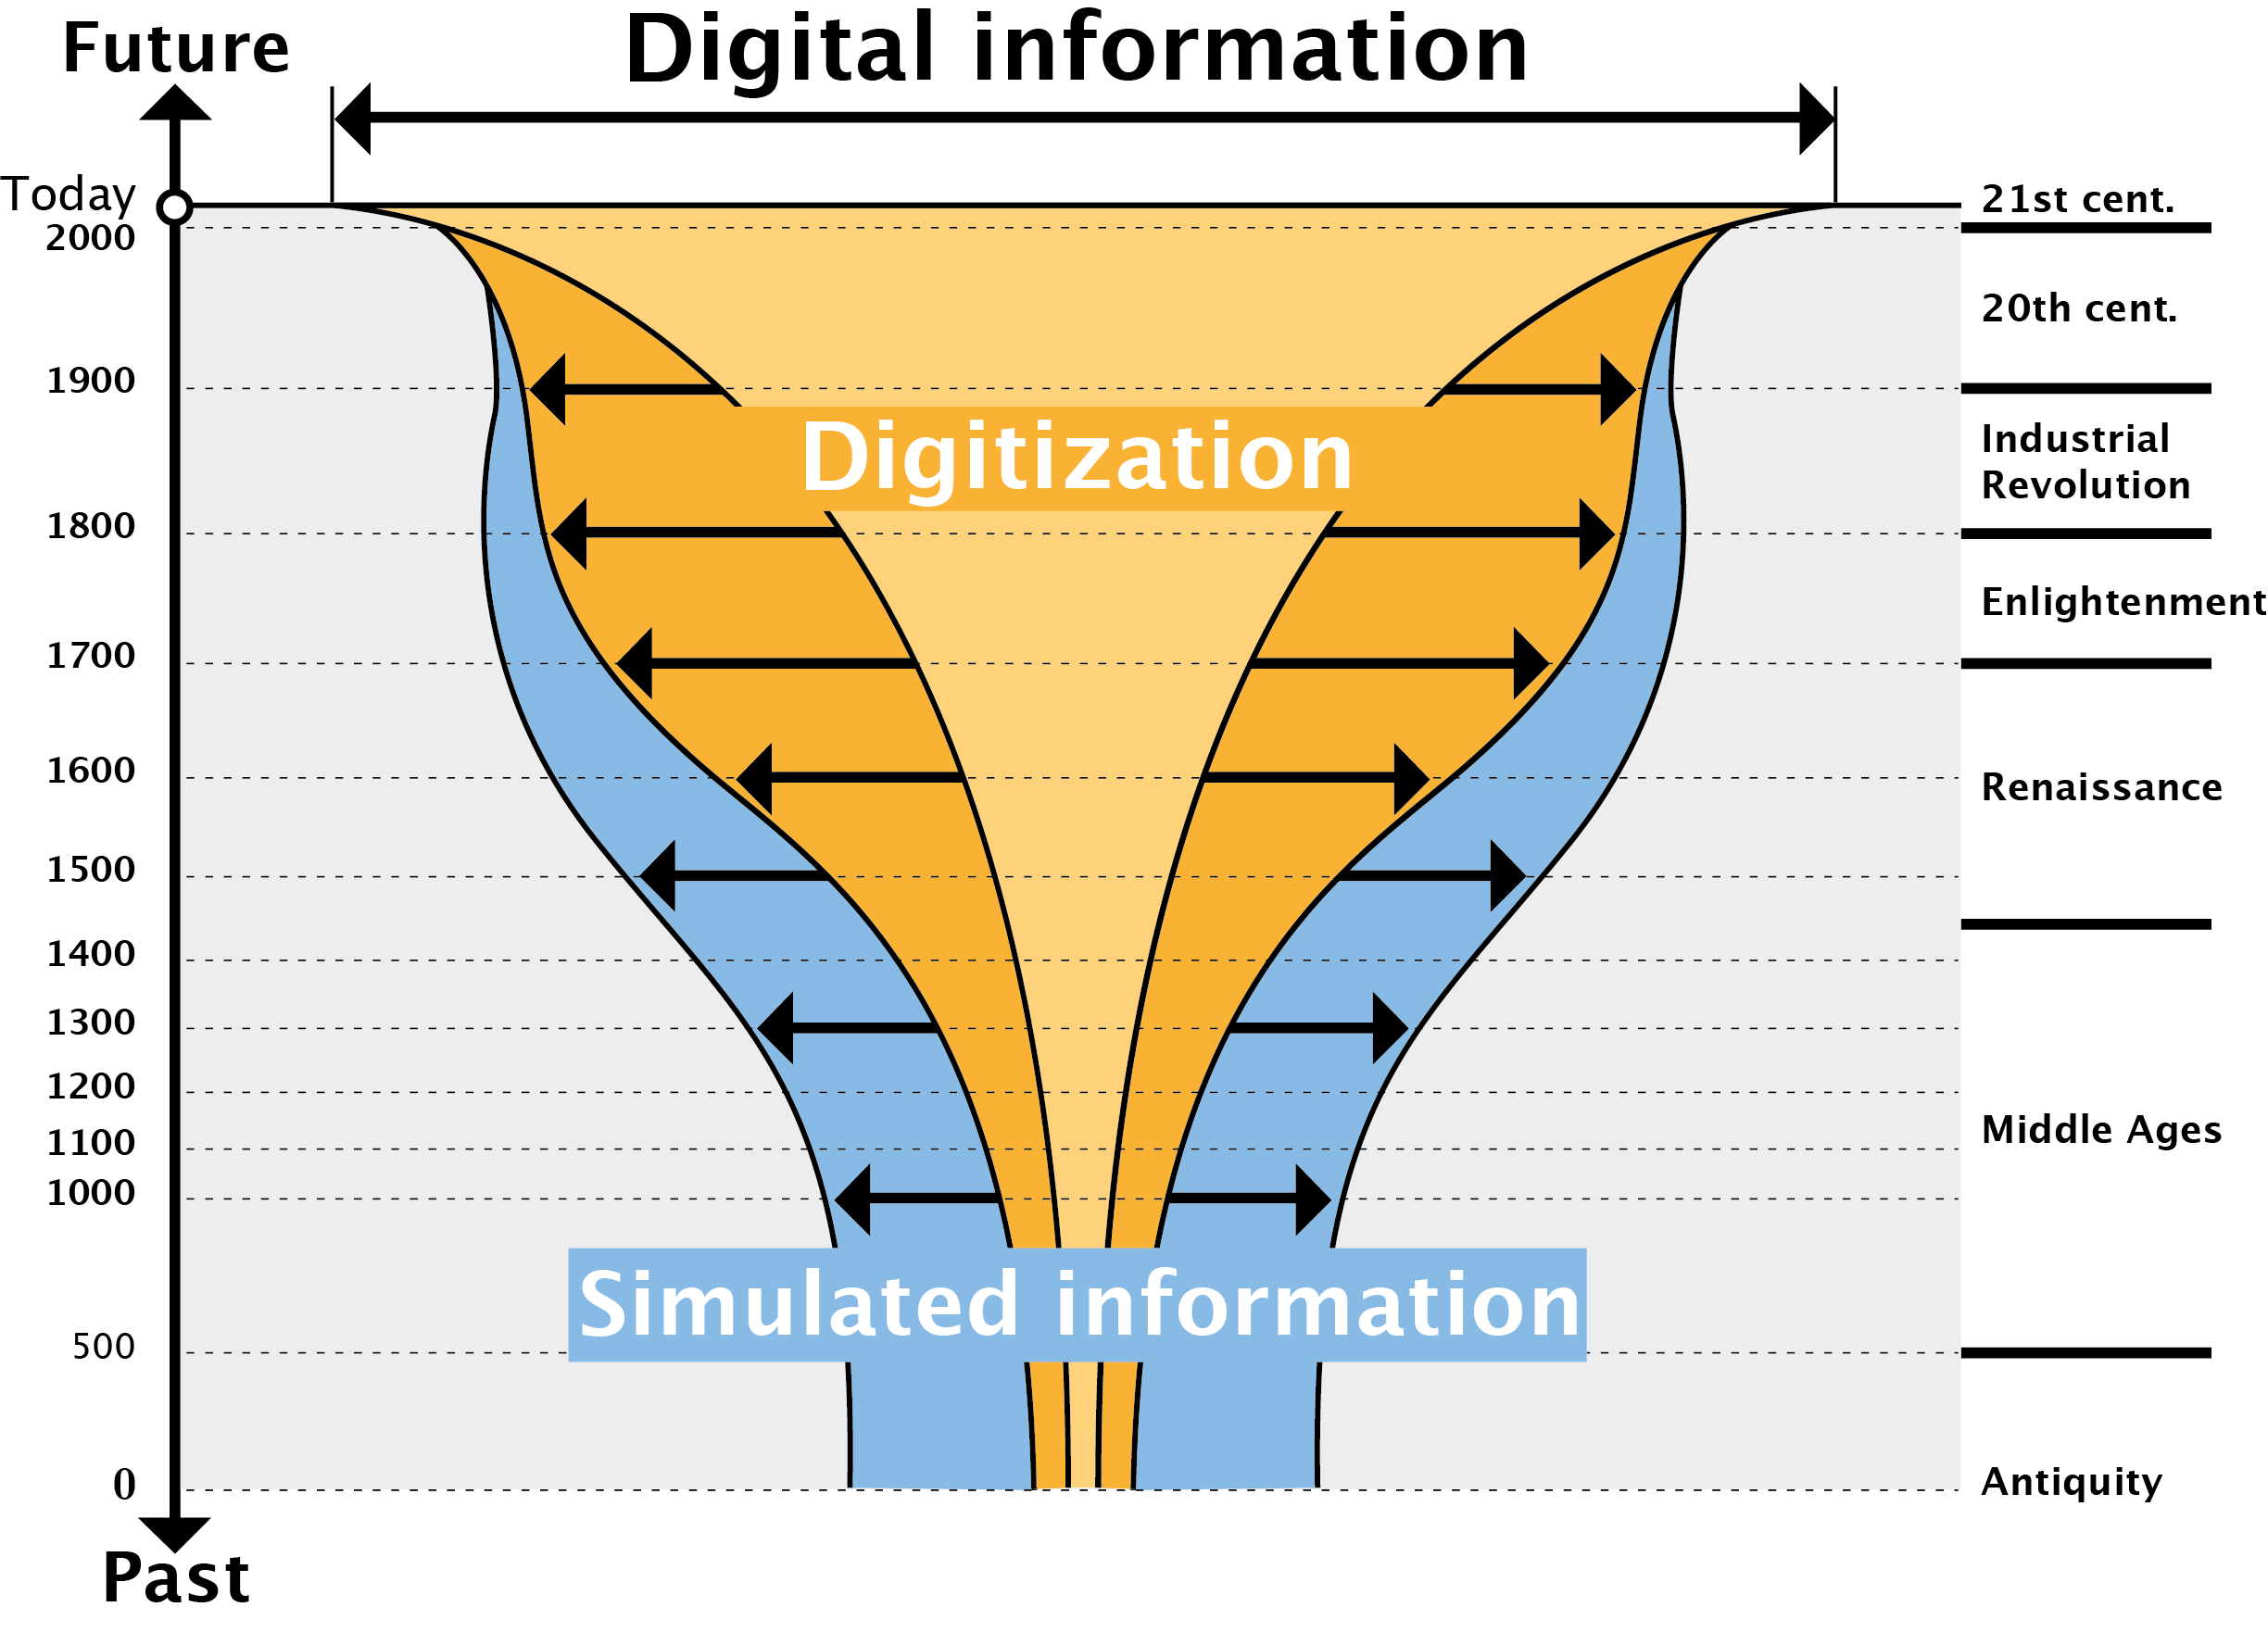
\includegraphics[width=\linewidth]{champignonKaplan.png}
 \legend{Legendary table}
  \end{sidecaption}
\end{figure}

Mais cela serait une erreur que de limiter l'application de ces nouveaux outils aux seuls stockages numériques récents, et ne pas citer l'importance du volume de connaissances collectionnées ces derniers siècles par certaines sciences sociales telles que l'archéologie ou encore la géographie. Des données qui n'attendent qu'à être cataloguées numériquement puis explorées dans le but d'en faire ressortir de nouveaux motifs. Voir la figure \ref{fig:I_Champi} \footnote{Voir l'article sur son blog \href{http://fkaplan.wordpress.com/2013/03/14/lancement-de-la-venice-time-machine/}{@FrédéricKaplan}}

%\begin{figure}[tb]
%\raggedright
%\begin{sidecaption}{This is a subcaption just for illustration purposes. This is a subcaption just for illustration purposes. 
%Champignon Informationnel de Frédéric Kaplan. Page number is \LARGE\textbf{\thepage}}[fig:test]
%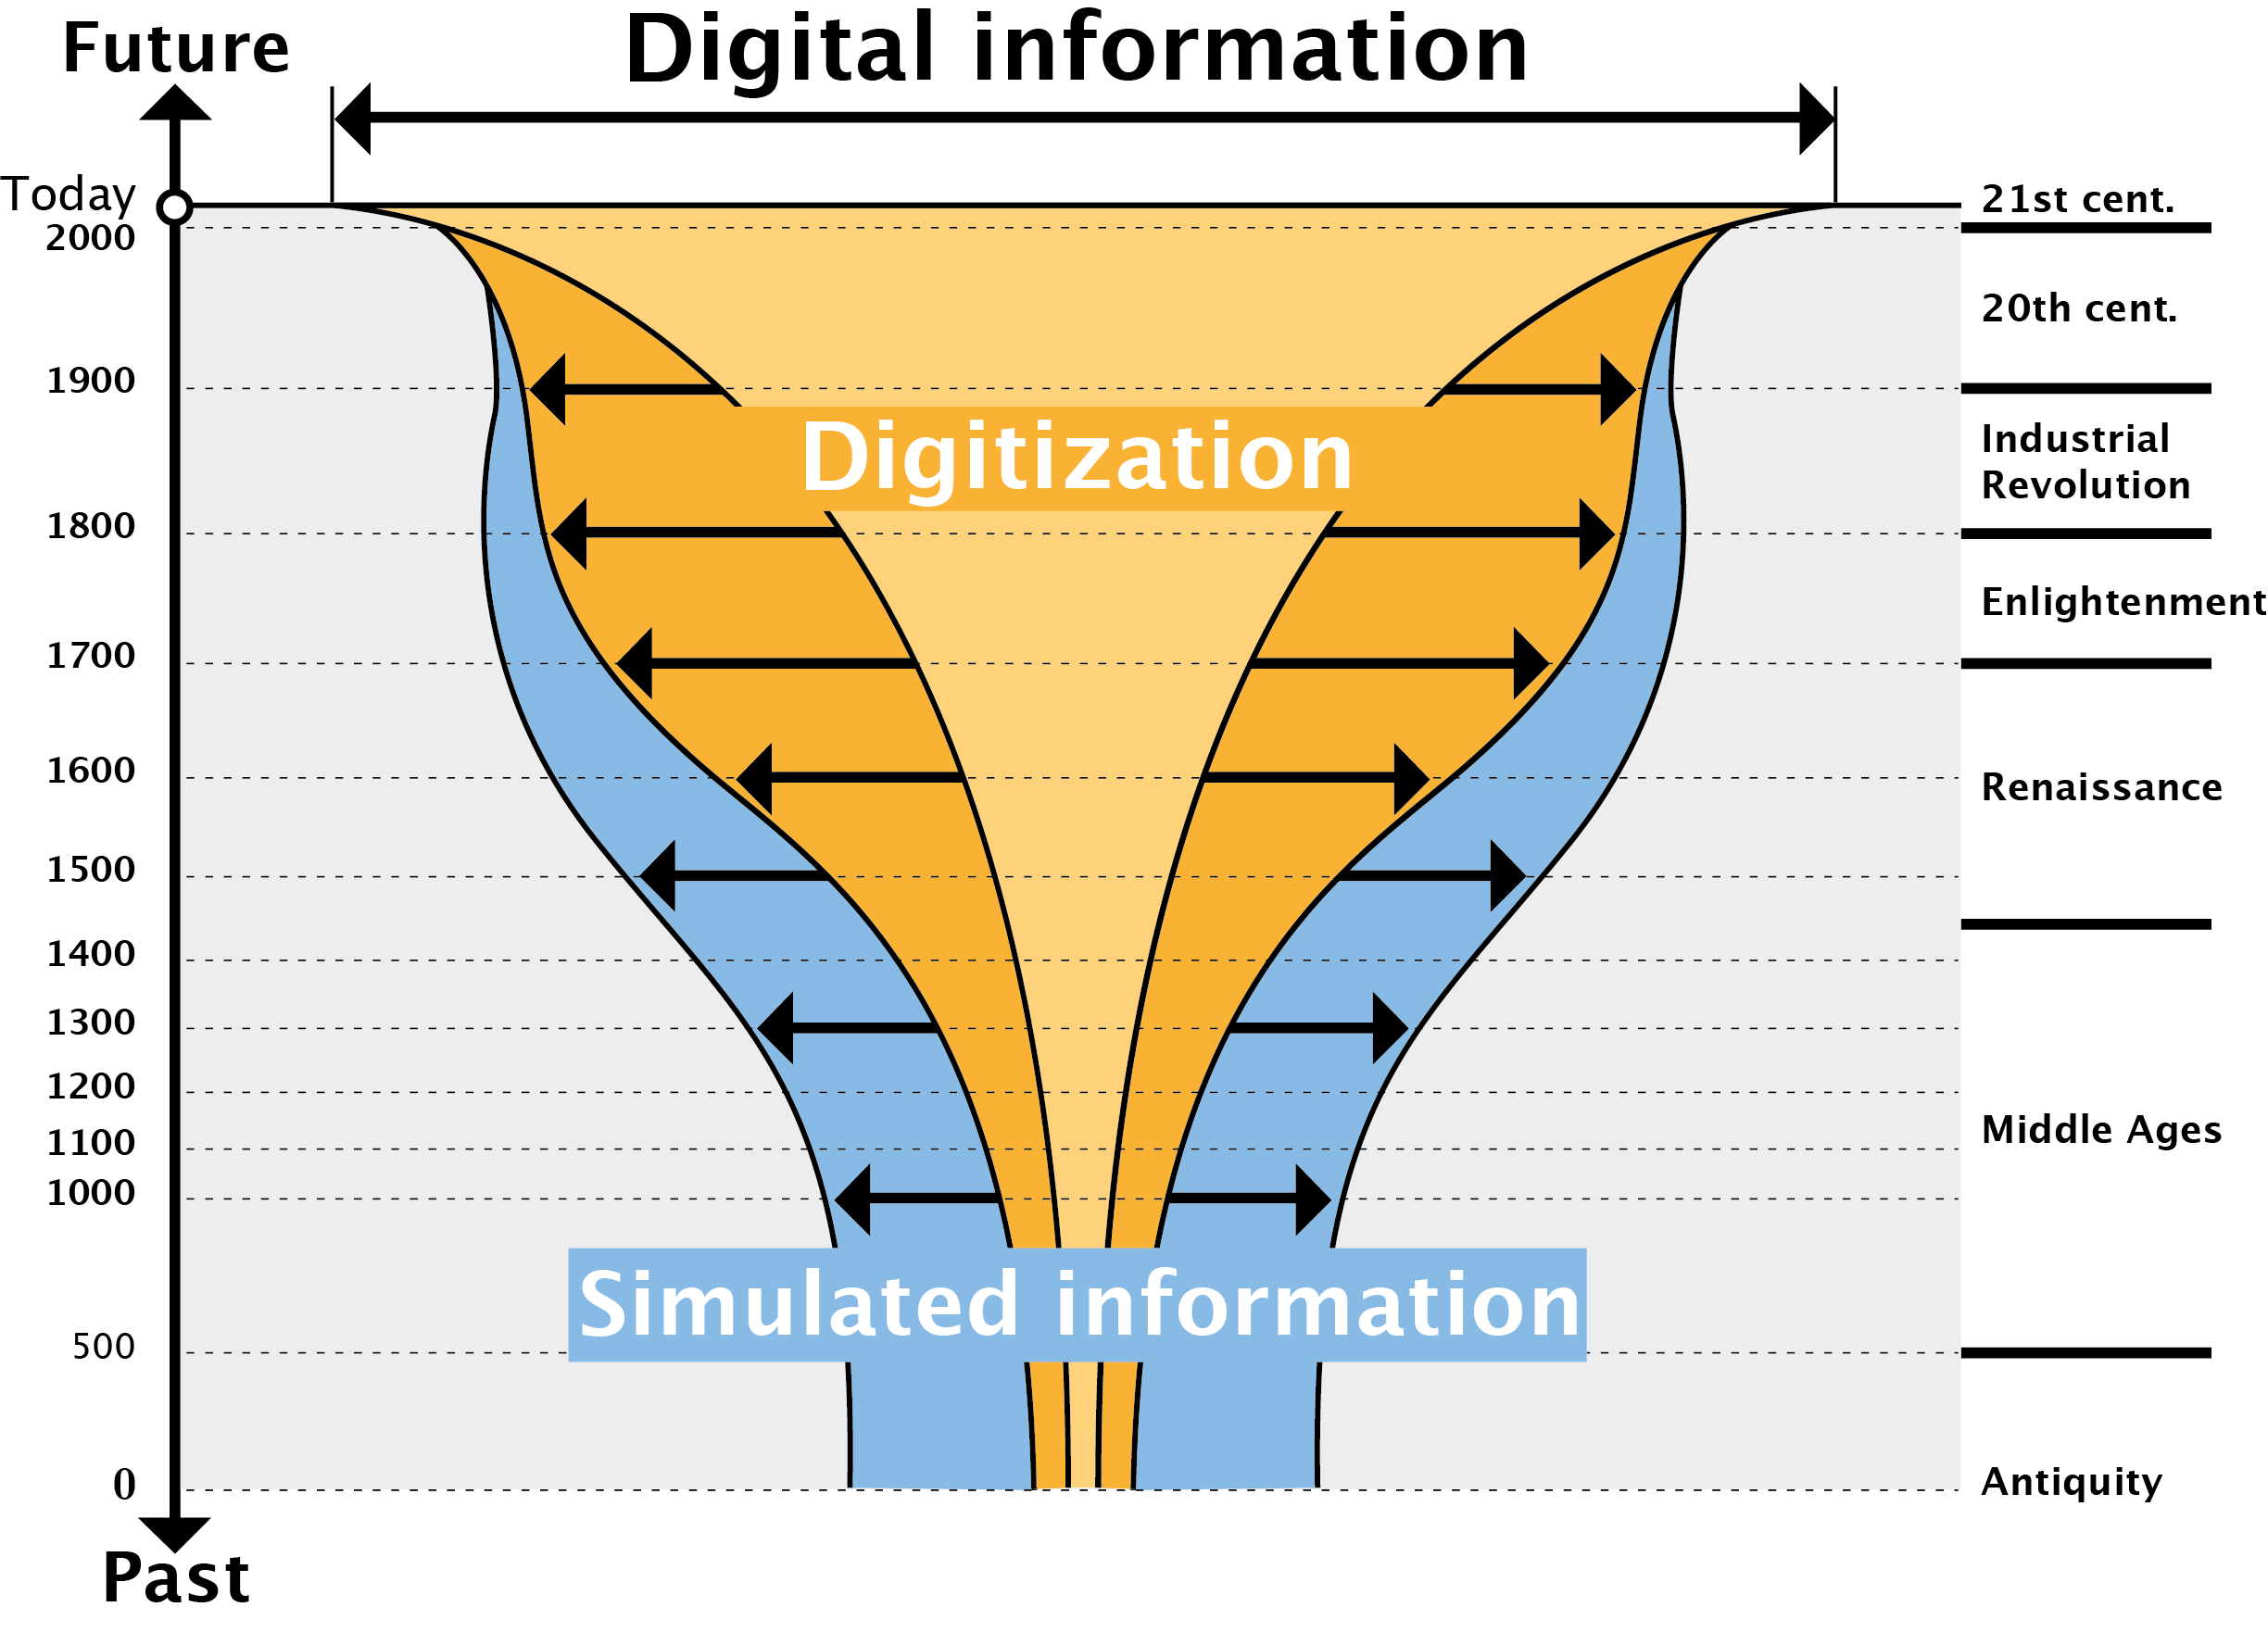
\includegraphics[width=\linewidth]{champignonKaplan.png}
%\end{sidecaption}
%\end{figure}

La classification automatique des données par l'ordinateur mais aussi la construction de modèles et leur simulation (au sens d'abord mathématique et parfois algorithmique du terme) apparaît rapidement comme un enjeux pour la géographie. La simulation de ces derniers apparaissant comme un outil de construction de connaissance absolument naturel et nécessaire pour confronter et construire les théories en rapport avec ces données \autocite{Kao1963, Hagerstrand1967b}. L'image de cette communauté inter-disciplinaire agitant et confrontant ses problématiques méthodologiques, techniques, théoriques dans un but de progression commun, fait écho à des revendications plus récentes \footnote{On pensera notamment à la communauté ABM inter-disciplinaire qui gravite autour de la revue JASSS fondée en  1990}. En réalité cet esprit de partage tient d'une \enquote{volonté commune} qui apparaît quasiment avec l'apparition et la démocratisation des techniques de simulation. C'est ainsi que l'on trouve trace des efforts de cette communauté de chercheurs dans plusieurs ouvrages tels que \autocite{Beshers1965,Naylor1966,Dutton1971,Guetzkow1962,Guetzkow1972}.

A ce sujet \textcite{Fleisher1965} produit une réflexion tout à fait remarquable par sa lucidité et son anticipation, comme en témoigne sa conclusion : \foreignquote{english}{I have argued that in the near future the social science will remain largely empirical and that simulation can serve as a device for making experiments \textbf{in vitro}. I think that this use is more important, at this time, than the massive making of models and that the principal contribution of simulation lies in the direction of intelligent, vivacious empiricism} \autocite{Fleisher1965}

%Forrester1969 a ce sujet "In the social sciences failure to understand systems is often blamed on inadequate data... The barrier is deficiency in the existing theory of structure." \autocite[355]{Batty1976}

\subsection{La diffusion d'un nouvel outil prometteur dans les sciences sociales : la simulation de modèle}

\subsubsection{Le contexte historique de l'après guerre favorable}

La plupart des disciplines connaissent une phase de transformation après les années 1950-60 qui va de pair avec la découverte de nouvelles méthodes quantitatives et la volonté d'opérer un rapprochement avec les techniques scientifiques de construction des connaissances communes aux sciences naturelles.

Paragraphe introductif des changement après guerre : La conjoncture politique favorable, L'apparition de mouvements inter-disciplinaires fédérateurs, L'influence de l'école néo-positiviste, l'émergence d'une pensée holiste dans les sciences...
%% FIXME

L'érosion d'un dogme dans les sciences naturelles; celui du déterminisme scientifique hérité de la pensée \enquote{classique} qui plonge de nombreuses disciplines en \enquote{crises} \autocite[20-23]{Pouvreau2013}. Une transition que l'on peut observer au travers de différents travaux majeurs, comme la statistique des lois de Boltzman pour la thermodynamique, ou le principe d’indétermination d'Heisenberg pour la mécanique quantique. Cette remise en cause peut également être associée à l'émergence d'une pensée \enquote{holiste} (ou pensée de la \enquote{totalité}) qui se construit en confrontation avec la pensée réductionniste historique.

%Il manque l'écologie, cf unwin1992 121

\subsubsection{Une polysémie des termes}

\paragraph{Définitions générales du terme \enquote{modèle}}

Une petite disgression temporelle dans notre argumentation permet de lever rapidement ce doute, si ces termes sont encore si polysémique à ce jour, ce n'est pas tant du fait de leur nature trop abstraite, mais au contraire du fait de leur richesse historique \textcite[131]{Varenne2012}, et de la grande variétés des pratiques qu'ils continuent de recouvrer dans l'ensemble des disciplines. Sur ce deuxième point, l'enrichissement et la mutation dans l'aception de ces termes \enquote{modèles} et \enquote{simulation} et de leur rapports, continue de se développer avec l'apport continue de nouveaux outils; des travaux récents de cataloguage \footnote{Voir par exemple les deux tomes \enquote{Modéliser \& Simuler} de \textcite{Varenne2013}, et la récente collection d'ouvrage \enquote{Modélisations, Simulations, Systèmes complexes (MS2C)} dédié depuis 2013 à ce champs de recherche spécifique qu'est l'épistémologie appliquée.}, préalable nécessaire à l'établissement de nouvelle typologies, sont à l'oeuvre pour tenter de caractériser ces changements, comme par exemple ceux de \textcite{Varenne2013}

La première définition généraliste et aussi la plus couramment encore rencontrée dans la littérature est probablement celle de Marvin Minsky établis en 1965 \autocite{Varenne2008} \autocite[15]{Varenne2013}  : \enquote{ Pour un observateur B, un objet A* est un modèle d’un objet A, dans la mesure où B peut utiliser A* pour répondre à des questions qui l’intéressent au sujet de A } \autocite{Minsky1965}

A partir de cette définition, Franck Varenne \autocite{Varenne2008} relève dans une analyse plus moderne du terme les cinq points suivants : 
\begin{enumerate}
  \item Le modèle n'est pas nécessairement une représentation
  \item Le modèle doit son existence à l'existence d'un observateur subjectif, et d'un questionnement lui aussi subjectif
  \item Le modèle est un objet qui a une vie propre, une existence autonome
  \item L'existence du modèle est justifiée par l'existence d'une \enquote{fonction de facilitation}
  \item Cette caractérisation minimale permet l'établissement d'une typologie
\end{enumerate}

Franck Varenne propose dans des travaux plus récents \autocite{Varenne2013} d'associer à cette définition les travaux de Mary S. Morgan et Margaret Morrison qui replace et caractérise le modèle dans une enquête de connaissance par la fonction de médiation (point 4 de la liste) qu'il investit, une façon de faire écho à la problématique motivant la construction de modèle établit dans la définition de Minsky.

Un modèle est ainsi définit comme \enquote{un objet médiateur qui a pour fonction de faciliter une opération cognitive dans le cadre d'un questionnement orienté}, opération cognitive qui peut être de cognition pratique (manipulation,  savoir-faire, apprentissage de gestes, de techniques, de conduites, etc.) ou théorique (récolte de données, formulation d'hypothèse, hypothèse de mécanismes théoriques, etc.) \autocite{Varenne2013}

Les travaux actuels de \textcite{Varenne2008, Varenne2013} dénombre pas moins de cinq familles pour un total de vingt grandes fonctions permet de situer efficacement la ou les problématiques - rien n’empêche les fonctions de se recouper - qui motivent la construction d'un modèle. 

\paragraph{Définition générale du terme \enquote{simulation}}

Le terme \enquote{simulation}, tout comme le terme \enquote{modèle}, est porteur d'une polysémie qui remonte aux alentours de son apparition en 1960. 

Bien que la simulation apparaisse sous sa première forme computationelle dans la technique de Monte-Carlo et les travaux de Von Neumann et Ulman \autocite{Eckhardt1987}, il faut attendre les années 1960 et les avancées techniques nécessaires pour que son utilisation semble utile. \textcite{Morgan2004} estime que le mot se diffuse vraiment dans la communauté inter-disciplinaire, et en économie, aux alentours de 1960. Il souligne le rôle central de Martin Shubik, un des pères de la théorie des jeux \footnote{voir sa \href{http://blogs.library.duke.edu/rubenstein/2012/12/18/the-martin-shubik-papers-from-early-game-theory-to-the-strategic-analysis-of-war/}{@Biographie}} dans la construction de ce débat autour de la notion \footnote{Shubick est aussi présent à un des tout premiers symposiums sur le sujet organisés par \textit{American Economic Review} \autocite{Shubik1960b}, ou il retrouve d'autres pionniers de son époque, comme \textcite{Orcutt1960}, et Simon \autocite{Clarkson1960}}, comme celui qui a servi à la fois d'intermédiaire important dans la rencontre entre les différents acteurs de l'économie expérimentale et de l'informatique, mais aussi comme celui tout aussi important de prospecteur au travers des vastes études bibliographiques qu'il a réalisé sur le sujet \autocite{Shubik1960a} \autocite{Shubik1972}, un travail toujours utile pour mieux juger de la polysémie du mot en cette période.

Par la suite d'autres conférences et ouvrages vont proposer de fixer, toujours dans une construction inter-disciplinaire, cet objet \enquote{simulation}, comme on peut le voir dans \autocite{Guetzkow1962, Guetzkow1972,Dutton1971}. Une polysémie qui même si elle a muté avec le temps, du fait de l'évolution des techniques et des pratiques, reste encore tout à fait d'actualités, et provoque toujours de large débats entre disciplines \autocite{Varenne2013}. Malgré cette hétérogénéité d'acceptation, la simulation computationnelle est rapidement reconnue par les disciplines en sciences sociales ou les sciences du comportement comme un outil important pour la construction et l'extension de théories (\textit{theory-building} ou \textit{model-building} selon la fonction définie pour le modèle), de par sa capacité à manipuler certes des symboles mathématiques, mais pas seulement \autocite[924-325]{Clarkson1960}. Pour ne pas trop mutiler notre objet d'étude par une définition trop restreinte, \enquote{la simulation de modèle} sera ici évoqué dans sa dimension avant tout numérique ou algorithmique (cf. dirigé par des règles) \autocite[36-38]{Varenne2013}.

\subsubsection{La simulation vue comme laboratoire virtuel d'expérimentation, une analogie ancienne}

Parmi la vingtaine de fonctions épistémiques recensées par \textcite[14-23]{Varenne2013} motivant la construction d'une simulation de modèles, la caractéristique la plus souvent exprimée pour l'époque en sciences sociales est sûrement cette capacité à pouvoir \enquote{expérimenter} sur les modèles en mobilisant des processus et des interactions sélectionnés et animés dans le cadre d'une dynamique, d'un temps mimant celui des systèmes cibles \footnote{Plusieurs auteurs, comme \autocite[462]{Gullahorn1965}, \autocite[296]{Doran1970}, \autocite[294-295]{Batty1976} semble faire référence implicite ou explicite à cette action de \enquote{plonger le modèle dans le temps}. Hors \autocite[31]{Varenne2013} indique que cette dénotation se rapporte principalement au temps du système cible, et non pas au temps du modèle, qui peut être simulé autrement (avec un tirage probabiliste).

Cette référence n'est donc pas un marqueur permettant de caractériser en elle même la notion de \enquote{simulation de modèle}, une métaphore à manipuler avec prudence donc.}, et cela même dans des conditions difficiles caractérisés par l'absence ou inconsistance des données, expérimentation réelles impossibles ou difficiles, etc. mais pas seulement, car la simulation de modèles a aussi vocation à simplifier certains simulations physiques coûteuses, ou trop limitées dans l'expression de nouvelles hypothèses. Ce lien entre simulation et expérimentation, complexe du fait de la relation entretenue entre le modèle et la réalité, est aussi ancien que la technique elle-même, Von Neumann affirmant dès le départ sa volonté de remplacer par des simulations sur ordinateur certaines techniques coûteuses de simulation physique \autocite[15]{Winsberg2013}.

Régulièrement employée dans la littérature, cette fonction d’expérimentation revient également sous la forme de \enquote{laboratoire virtuel}, un terme qui prend selon les époques des teintes légèrement différentes, et cela quelque soit les techniques sous-jacentes support à la simulation des modèles.

Parfois le terme est invoqué directement, parfois il est implicite au discours présenté. Pour ne citer que quelques auteurs pionniers dans l'historique de la notion, les premier ouvrages collectifs en simulation et science sociale de \textcite{Guetzkow1962, Guetzkow1972} \footnote{La légende veut que l'idée d'appliquer la simulation aux \textit{Behavioral Science} viendrait d'un déjeuner entre Guetzkow et des physiciens nucléaire lors de son séjour au Carnegie, pour en savoir plus : \href{http://www.hawaii.edu/intlrel/pols635f/Guetzkow/hg.html}{@Harold} } et les travaux de Herbert Simon; et de façon plus localisé, en économie \textcite[915]{Shubik1960b}, en psychologie sociale \textcite{Abelson1968} \footnote{Un auteur connu aussi pour avoir échangé aussi avec \textcite{Boudon1967} sur la simulation à la même période, voir  \textcite{Padioleau1969}}, \textcite{Fleisher1965} météorologue, le couple d'Anthropologues/sociologues du comportement \textcite{Gullahorn1965}, l'archéologue anthropologue et informaticien \textcite{Doran1970}, la physicienne biostatisticienne et démographe \textcite{Sheps1971}, l'informaticien \textcite[3-4]{Forrester1971}, l'économiste informaticien \textcite{Naylor1966}, le professeur de science régionale \textcite[271]{Harris1966}, l'urbaniste \textcite[295]{Batty1976} sans oublier plus récemment \textcite{Epstein1996}, l'écologue \textcite{Grimm2006}, et encore sûrement bien d'autres...

L'analogie bien que pratique, et illustrative d'une certaine réalité dont on n'aurait bien du mal à nier l'existence tant celle çi est persistente dans la littérature, mérite toutefois d'être étudié plus en détail par la suite. Les récente et au moins tout aussi récurrente critique sur l'apport d'une telle expérimentation dans les sciences sociales montre qu'il est intéressant de développer quels sont véritablement ces points de similitudes et de divergences entre l'expérimentation physique et virtuelle, ne serait ce que pour construire une argumentation lisible à destination des nouveaux modélisateurs. Des sociologues des sciences comme Bruno Latour ou Ian Hacking ont développé ces vingt dernières années une véritable épistémologie des pratiques de laboratoire centrés autour de la démarche expérimentale, des réflexions qu'il nous faut prendre absolument prendre en compte pour tout analyse qui se voudrait plus poussé sur cette notion, comme en témoigne les travaux récents des épistémologues spécialisé dans la simulation comme Winsberg, ou \textcite[204]{Varenne2012}

\hl{A linker avec la partie épistémo de la fin du chapitre 1 ! }

\subsubsection{Un engouement pour la simulation qui touche l'ensemble des sciences sociales}

Cet engouement pour la simulation de modèles touche toute les sciences sociales ou presque, comme en témoigne cet état de l'art sur le sujet prenant pour étude la période 1950-1970.

Suite au mouvement Cybernétique, à la convergence des travaux sur l'intelligence artificielle et les sciences cognitives, les premiers travaux qui visent la démonstration de la faisabilité de la simulation dans la discipline viennent de Newell, Shaw, et Simon à la fin des 1950 \autocite{Gullahorn1965} \footnote{Avec plusieurs tentatives pour la construction d'une machine universelle de résolution de problème (\foreignquote{english}{Logic Theorist program} en 1957 et \foreignquote{english}{General Problem Solver} en 1959). Ce programme s'avère également être la première pierre posé de la l'intelligence artificielle, en formation à l'intersection de la naissance encore récentes des science cognitive et de l'informatique. Cette machine est conçu pour mimer les capacités de résolutions de l'esprit humain, et permet enfin d'exprimer et de questionner les théories comportementales dans un langage informatique alors plus précis et moins ambigu que le langage naturel. Le programme est ainsi capable de résoudre des problèmes aussi différents que de jouer aux échec, de résoudre des problèmes mathématiques,  ou de retrouver des motifs dans des données.} A ces travaux s'ajoutent ceux répétés de Hovland en 1960 puis de \textcite{Abelson1968} qui encourage l'utilisation de la simulation pour la construction théorique de ce que \textcite{Ostrom1988} appellera \foreignquote{latin}{a posteriori} les \foreignquote{english}{complex human processess }. La simulation est également utilisée en psychologie pour formuler et vérifier des théories sur les comportements sociaux \autocite{Gullahorn1965a} \footnote{ comme par exemple le modèle Homonculus développé par Gullahorn pour tenter de mieux comprendre les stratégies de résolution de conflits avec la programmation de comportements au niveau individuel \autocite{Gullahorn1965} }

En sociologie, James Coleman \foreignquote{english}[Guetzkow1972 36]{considered it as a half-way point between verbal speculative theory and formal theory, aiding in the development of such theory through concretizing the functioning of social processes.}

En archéologie \footnote{On pourra trouver plus d'information via \autocite{Kohler2011}, et \autocite{Lake2013}}, l'arrivée des outils statistiques \footnote{\foreignquote{english}{Similar trends are apparent in allied subjects such as anthropology and social geography. In particular, location analysis has influenced archaeologists, with its emphasis on the study of all aspects of a population and its environment, and on the use of quantitative methods and models (Haggett 1963)} \autocite{Doran1970}} et de la pensée systémique \autocite{Flannery1968, Binford1968} \footnote{Une analyse a posteriori confirme l'apport de la systémique dans la construction des modèles de simulation, comme en témoigne \textcite{Aldenderfer1998} en 1988. \foreignquote{english}{One of the theoretical hallmarks of the \textit{New Archaeology} was the systems approach \autocite{Aldenderfer1991}, and a result of its adoption was the use of computer simulation to model whole societies or significant portions of them.}} par transfert d'autres disciplines, comme la géographie, va introduire une rupture dans les pratiques de la discipline. 

% VOir aussi Mathematics and Computers in Archaeology doran 1975, partie sur la simulation cf http://books.google.fr/books?id=ZAPvXcnz0kkC&pg=PA369&lpg=PA369&dq=The+computer+in+archaeology:+A+critical+survey+whallon&source=bl&ots=6et-F8jHab&sig=gQWgTIHRuO2ICqMJtrRdGovo9gs&hl=fr&sa=X&ei=OskxU5W5Nen20gW0_4DIDA&ved=0CGUQ6AEwBQ#v=onepage&q=whallon&f=false

Une remise en question équivalente à celle rencontrée par la géographie durant les années 1960-1970, durant laquelle des auteurs comme \textcite{Clarke1968} ou \textcite{Doran1970} vont militer pour l'utilisation de modèles de simulation dans la discipline. Militantisme qui semble recevoir un écho positif tout au long des années 1970, certains auteurs comme \textcite[38]{Whallon1972} n'hésitant pas à définir \footnote{ \foreigntextquote{english}[Whallon1972, 38]{The techniques and procedures of computer simulation so closely parallel the current thinking and processes of model- building of many archaeologists that the lateness and limits of their application are surprising.}} la simulation comme un prolongement naturel à la pratique existante de construction des modèles. Cette mise en oeuvre de programmes pionniers se poursuit avec une diversification dans les usages jusqu'au début des années 80 et constitue une première phase d'appréhension de la simulation, plus que d'une adoption massive par la discipline. \autocite{Lake2013}

%\autocite{Clarke1987}
A la croisée de plusieurs disciplines, sociologie, anthropologie et géographie on trouve les modèles de variation de population, ou modèle démographiques dont les hypothèses sont amenées à varier selon des facteurs biologiques, économiques, spatiaux faisant souvent appel à une dynamique des interactions humaines impossible à expérimenter dans la réalité. \footnote {\foreignquote{english}{To understand how changes in the size and composition of human populations occur, it is essential to study the determinants of these changes and the interrelations among them. The impossibility of investigating these relationships experimentally stimulates the formulation of models, as a means of enhancing our understanding of the process.} \autocite{Sheps1971}} Dans cette branche se cotoient donc macro-simulation, micro-simulation et modèle analytique hérités des premiers démographes mathématiciens, comme le plus connus d'entre eux, Lotka dont les premières publications sur le sujet date de 1907. \autocite[355]{Veron2009}

%%FIXME 
Les modèles TRIM, puis DYNASIM (entre 69 et 75) développés par Orcutt et son équipe au \foreignquote{english}{Urban Institute} sont pionniers \autocite{Orcutt1957, Orcutt1960, Orcutt1976}, et inspirent différents modèles dynamiques en démographie avec les travaux de \autocite{Perrin1964}, \textcite{Sheps1971}, et \textcite{Ridley1966} avec REPSIM aux États-unis,  \textcite{Hyrenius1964} en Suède, \textcite{Horvitz1971} avec POPSIM, ou encore SOCSIM basé sur les travaux en anthropologie de \textcite{Gilbert1966}, qui viennent compléter efficacement les modèles analytiques inspirés des travaux de Lotka \autocite{Sheps1971}, père entre autre de la démographie mathématique moderne. Coïncidence de l'histoire, ou inspiration commune, Hägerstrand apportera de façon parallèle en géographie, et dans la même décennie \autocite{Hagerstrand1952, Hagerstrand1967}, une vision micro similaire, à cela près qu'elle y ajoute un ancrage spatial des individus.

Dans le cas de l'anthropologie, qui partage un tronc commun avec nombre de problématiques en archéologie, et en psychologie, on retiendra le manuel édité par \textcite{Hymes1965} retranscrivant une conférence de 1962. Celui-ci contient deux articles importants pour la discipline, celui de \textcite{Gullahorn1965} et celui complémentaire de \textcite{Hays1965}. L'intégration de la simulation dans l'arsenal méthodologique prend part selon \textcite[274]{Bentley2009} d'un mouvement ayant pour objectif de mieux comprendre les contraintes sociales et culturelles dans les processus démographiques en général. Dans ce cadre par exemple de l'étude de la parenté ou \foreignquote{english}{kinship}, l'application de la simulation donne lieu à plusieurs expériences pionnières \autocite{Dyke1981} en simulation comme celle de \textcite{Kunstadter1963}, mais aussi de \textcite{Gilbert1966}. Cet engouement continuera dans les années 1970 \autocite{Read1999} avec des simulations mettant en œuvre des processus stochastiques dynamiques comme par exemple dans les travaux de \textcite{Howell1978} et \textcite{Thomas1973}.

%\autocite{Costopoulos2007} . %Antony Wallace également, levy strauss 1955: les mathémztique de l'homme...

%En utilisant la simulation non pas comme un solveur d'équation mais en utilisant la puissance des opérateurs symboliques à sa disposition pour la mise en temporalités de systèmes d'interaction dans des sociétés passés, Doran décrit une vision de la simulation qui n'est pas sans rapeller le multi-agent d'aujourd'hui. Une conception de la simulation reprise et concrétisé par DH Thomas en 1972.\footnote{La discussion sur  \href{www.jiscmail.ac.uk/cgi-bin/webadmin?A2=ind04\&L=simsoc\&F=\&S=\&P=39083} {@SimSOC}} 

\begin{framewithtitle}[Les premiers langages de programmation]{ Les premiers langage de programmation }

La période 1955 - 1965 est une période de recherche caractérisée par la reconnaissance de la simulation pour résoudre un certain nombres de problèmes difficilement tractables mathématiquement.\autocite{Nance1993, Ackoff1961} Les programmes de développement visant à la mise en place de modèles de représentation, de description nécessaire et facilitant pour la construction de simulations se multiplient. Deux classes de langage informatiques vont voir le jour durant cette période, et vont continuer à se développer et à s'influencer chacune de leur coté jusqu'à encore aujourd'hui. D'une part, les langages de plus haut niveau qui apparaissent ont pour vocation de se positionner comme une alternative plus expressive que l'assembleur. Dans cette optique le premier compilateur FORTRAN apparaît en 1957,  Algol en 1958, Cobol en 1959, et Lisp 1958. Ces langages et leur successeurs sont d'usage assez générique, et permettent de décrire correctement tout types de programmes. Toutefois à l'époque de leur apparition ils sont d'accès relativement difficiles pour une personne non initiée, ce qui nous amène au développements sur la même période d'une deuxième catégorie de langage, plus spécialisée dans la construction spécifique de modèle de simulation. \autocite[239]{Naylor1966}

A la même époque, des langages spécialisés dans l'expression des simulations apparaissent, et pour la plupart s'appuient et évoluent en parallèle des développement des langages classiques sur lesquels ils s'appuient. Ces SPL ( \foreignquote{english}{Simulation Programming Langages}) comme Simula en 1962, ou bien Dynamo en 1958 ont ceci d'intéressant qu'ils ont très largement accompagné les formidables avancées conceptuelles de cette époque et cela au travers des différentes disciplines. Ainsi la première période 1955-1960 est marqué par la mise au point de GSP (\foreignquote{english}{General Simulation Program}) par Owen et Tocher \autocite{Tocher1960}. Celui-ci est considéré comme le tout premier langage mis au point pour faciliter la description de simulation sur ordinateur. Un effort que Tocher va accompagner d'une publication phare en 1963 dans le livre \foreignquote{english}{Art of Simulation} \autocite{Tocher1963} . Vient ensuite une autre génération de langage en 1960-1965 comme GPSS (\foreignquote{english}{General Purpose System Simulator}), Simscript (développé sous l'impulsion de la RAND corporation), et la première version du langage SIMULA, qui donnera naissance à la fin des années 1960 à Simula-67, un langage qui aura un impact dépassant largement la classe des SPL, et inspirera les créateurs des futurs langages objets comme Alan Kay, auteur plus connu comme le créateur du premier langage objet SmallTalk. 

\end{framewithtitle}

% http://books.google.fr/books?id=G8sA95bz5pwC&pg=PA143&lpg=PA143&dq=%22Social+Physics%22+stewart+cybernetics&source=bl&ots=FsOC2mqHvr&sig=cS914G7pelGvgG6bG32fKsmWWPc&hl=fr&sa=X&ei=yTRAU5m7OIOH0AXwtYEY&ved=0CDsQ6AEwAQ#v=onepage&q=%22Social%20Physics%22%20stewart%20cybernetics&f=false
% "Social Physics" stewart cybernetics
% http://www.eoht.info/page/Princeton+Department+of+Social+Physics
% http://books.google.fr/books?id=F84mS2nnjWsC&pg=PA105&lpg=PA105&dq=geographer+reino+ajo&source=bl&ots=buVSBElr7Y&sig=_NXU0Py2goM2c6fVi1To3dUwqHQ&hl=fr&sa=X&ei=0DBAU_niJqrO0AWk44CwCw&ved=0CG8Q6AEwBw#v=onepage&q=geographer%20reino%20ajo&f=false
% http://www.persee.fr/web/revues/home/prescript/article/ingeo_0020-0093_1957_num_21_5_6491_t1_0223_0000_5#
% http://www.eoht.info/page/Social+physics
% Contributions to "social Physics" reino ajo
% Stewart, J.Q. "The Development of Social Physics"

\subsection{Les débuts de la simulation de modèle en géographie}

\hl{Bla bla ackerman retard de la géographie ... cybernétique ... etc.}

\subsubsection{Une \enquote{révolution quantitative} au coeur de multiples convergences}

L'apparition et la diffusion de ces techniques quantitative n'est pas le résultat d'une convergence unique, mais bien d'une succession de moments dont la fréquence et l'étalement temporel est difficile à cerner et empêche sur ce sujet toute exhaustivité. 

On retiendra toutefois plusieurs grands facteurs, à la fois généraux, et d'autres plus spécifiques à la géographie, dont certains qui peuvent paraître étonnamment antinomiques. Une convergence qui s'illustre dans la richesse et la diversité des transformations qui touche la discipline géographique entre 1950 et 1970, un constat déjà établi par bien d'autres auteurs \autocite{Varenne2014}

[28-29]Claval2003
%http://books.google.fr/books?id=s5xjIsejTjkC&pg=PA28&lpg=PA28&dq=h%C3%A4gerstrand+positivism&source=bl&ots=FrIMA95glO&sig=9Knqs1cLfJJefcc30qwsIMDzW-s&hl=fr&sa=X&ei=UMVDU86hJ-mS1AWPmIDoCw&ved=0CC4Q6AEwADgK#v=onepage&q=h%C3%A4gerstrand%20positivism&f=false

\paragraph{L'influence de l'école néo-positiviste}

%%RETRAVAIL A FAIRE
Le néo-positivisme, néo-empirisme, positivisme logique selon les étiquettes, est un mouvement philosophique important, sinon peut être le plus important, entre les deux guerres. Ce cercle dont on trouve les premières traces dans les années 1908 à Vienne, est organisé autour de grand débats, dont la caractéristique est d'être fréquenté par un grand nombre d'intellectuels provenant de toute disciplines. Tout au long de son évolution caractérisé par différentes phases (avec une apogée durant la troisième phase entre 1928-1934), de multiples courants d'opinions \textcite[126]{Ouelbani2006} vont être amenés à se cotoyer, du fait des débats internes, mais aussi des critiques extérieures au cercle. C'est donc à ce titre que \textcite[11]{Ouelbani2006}, préfère parler de \enquote{programme néo-positiviste} \footnote{Le programme de Carnap tient en quatre points selon Dahms, cités par \textcite{Ouelbani2006} : (i) la réduction de la philosophie à une théorie de la connaissance; (ii) la distinction des sciences, non plus en sciences de la nature et sciences humaines, mais en sciences empiriques et analytiques: (iii) le logicisme comme programme de réduction des sciences analytiques; (iv) le réductionnisme comme programme de réduction des sciences synthétiques ou empiriques.} plutôt que d'un réel courant unifié.

Inspirée des sciences naturelles, et plus particulièrement d'un observation des sciences physiques et mathématiques,  les tenants du programme néo-positivistes sont motivés par l'unification des sciences, et pensent l'application d'un tel programme incontournable pour fonder des sciences sociales véritablement \enquote{scientifique}. \textcite[1-20]{Ouelbani2006}

Les positivistes logiques ont ceci de particulier qu'ils raisonnent sur des démonstrations logiques encapsulant les énoncés observationels décrit dans une logique formelle qu'ils veulent non ambigue. Entre empirisme et logicisme, ce programme réductioniste fait porter toute la connaissance sur l'expérience; ce qui mène avec l'aide de l'analyse logique et mathématique à l'élimination de toute métaphysique, et de toute structure a priori (anti-kantien) dans la construction des énoncés d'observation. Ainsi l'inférence déductive se fait seulement sur des énoncés d'observations qui sont \foreignquote{latin}{a posteriori} tout à fait justifiable, et donc mobilisable dans celle ci que si ils sont \foreignquote{latin}{a priori} vérifiable.

Ian Hacking \autocite{Hacking1983} a selon Orain \footnote{Voir les notes de \href{http://www.esprit-critique.net/article-12642840.html}{@cours} dispensés sur le blog \enquote{esprit critique} de Olivier Orain} très bien saisi ce qui fait les axes communs \footnote{Le positivisme peut se définir par quelques idées forces. (1) L’importance accordée à la vérification (ou à une variante comme la falsification) : une proposition n’a de sens que si l’on peut, d’une quelconque manière, établir sa vérité ou sa fausseté. (2) La priorité accordée à l’observation : ce que nous pouvons voir, toucher ou sentir fournit, sauf pour les mathématiques, la matière ou le fondement le plus appréciable de la connaissance. (3) L’opposition à la cause : dans la nature, on ne trouve pas de causalité dépassant ou surpassant la constance avec laquelle des événements d’un certain type sont suivis par des événements d’un autre type. (4) Le rôle mineur joué par l’explication : expliquer peut contribuer à organiser des phénomènes mais le pourquoi reste sans réponse. On peut seulement remarquer que le phénomène se produit régulièrement de telle ou telle manière. (5) Opposition aux entités théoriques : les positivistes ont tendance à être non réalistes parce qu’ils limitent la réalité à ce qui est observable mais aussi parce qu’ils s’opposent à la causalité et se méfient des explications. Leur rejet de la causalité les fait douter de l’existence des électrons simplement parce que ces derniers ont une action causale. Ils soutiennent qu’il s’agit là seulement de régularités constantes entre phénomènes. (6) L’opposition à la métaphysique est finalement le dénominateur commun entre les points (1) à (5) ci-dessus. Propositions invérifiables, entités inobservables, causes, explications profondes, tout cela, dit le positiviste, est objet de métaphysique et doit être abandonné. \autocite[82]{Hacking1983}.} des différentes relectures du terme positivisme. Une parenté qui dans le cas du programme néo-positiviste est difficile à isoler tant l'aceptation par les proches (comme Popper) ou membres du programme (certain préféreront même le terme empirisme logique) est amenés à varier, on pourra ainsi se référer à la classification proposé par Hacking pour en savoir plus sur ce sujet. \autocite[81-86]{Hacking1983}

L'apogée du groupe à Vienne est de courte durée, avec les pressions du régime nazi et l'annexion de l'autriche le groupe est dissous. De nombreux acteurs du mouvement sont alors contraint à l'exil, et nombreux sont ceux qui vont aux États-Unis. A ce moment ce programme philosophique est alors quasiment inconnu des philosophes pragmatistes américain, mais paradoxalement il va trouver sur ce nouveau territoire un très bon accueil. 

C'est sur cette philosophie pragmatique depuis longtemps installé (Peirce, Dewey) que vient se greffer ce nouveau programme, jusqu'à finalement quasiment l'eclipser. Un transfert que l'on imagine pas totalement unilatéral, et il est presque évident que le discours originel Viennois tire largement profit d'une philosophie pragmatiste compatible dans ses fondements \footnote{ Ainsi selon \textcite[149]{Ouelbani2006} Carnap aurait été rassuré en 1935, date de son arrivée aux Etats-Unis, \enquote{ [...] de trouver une ambiance philosophique différente,en ce sens que les jeunes philosophes étaient intéréssés par des méthodes scientifiques et logiques}}. C'est ce que \textcite[123]{Wilson1995} affirme en disant que les pragmatistes \foreignquote{english}{[...] had created the conditions in which logical positivism and other analytic philosophies could flourish and ultimately displace them as the dominant voice in mid-century philosophical debates} mais aussi les conditions de son dépassement \foreignquote{english}{Pragmatism, then, not only created the conditions in which logical positivism and analytic philosophy could flourish in the United States, it also contained the seeds of the postanalytic philosophies that have attempted to move beyond [...] }. Ce programme va se diffuser à la fois sur les bancs des universités, mais aussi via les grand instituts scientifique après guerre qui font publicité de cette science \foreignquote{english}{mainstream}, organisés aux états-unis autour de l'ordinateur. 

La RAND fait partie de ses instituts fondé après guerre, qui approche dès 1947 les sciences sociales \autocite{Rand106}, et n'hésitent pas à mettre en avant par la suite les stars de la philosophie positiviste de l'époque comme Reichenbach. \autocite[384-385]{Barnes2011} 

\paragraph{L'apparition de mouvements inter-disciplinaires fédérateurs}

L'apparition de grands mouvements de convergence inter-disciplinaires et leur intérêt pour l'application de nouveaux concepts et techniques aux science sociales, dont certains prennent par la suite la forme de paradigme du fait de leur portée d'application : Cybernétique de Wiener, \textit{projet} de la \foreignquote{english}{General System Theory} de Bertalanffy \autocite[9]{Pouvreau2013} s'organise autour de grandes structures de recherches comme le MIT, la RAND, qui favorise les collaborations par la mise en place d'équipe de travail pluri-disciplinaire.

Parmis les ramifications directes de ces coopérations, la \enquote{social physics} de Stewart \autocite{Stewart1947}. Par la suite et surement du fait des liens développés à l'université de Pennsylvanie, lieu de ses études, et siège de la fondation de la science régionale d'Isard en 1954, Stewart sera amené à publier dans la revue \textit{Regional Sciences} \autocite{Stewart1958}.

Les retombées de ces interactions sur la géographie sont importantes \footnote{ A condition de ne pas oublier qu'une partie de ces concepts existent de façon sous-jacente aux disciplines, ce qui explique parfois leur rapidité d'acceptation. C'est le cas de l'approche systémique développé par la cybernétique quand elle ne fait pas qu'apposer un nom commun sur des concepts déjà étudiés, fait alors écho à des révolution méthodologiques en attente d'être activés. \textcite[5]{Batty1976} résume la situation ainsi \foreignquote{english}{The idea of systems being described in terms of structure and behaviour, in terms of input and output, and the notion of purposeful control of such systems in terms of negative and positive feedbacks, appeared to many social scientists an ideal description of their systems of interest and thus the approach has come to be used in more-or-less all of the social sciences}.}, et fournissent tout autant : (i) des concepts généraux en correspondances avec les débats qui anime l'ensemble des sciences : sensibilité aux conditions initiales, équifinalité, bifurcation et catastrophe, boite noire, rétro-causalité, hiérarchie d'emboitement, etc.) , (ii) un catalogue d'isomorphisme supplémentaire dont la correspondance reste à évaluer dans notre discipline \autocite{Wilson1969}, (iii)  une méthodologie et une typologie des modèles tirés de la recherche opérationnelle \autocite{Ackoff1962} \footnote{Une discipline proche du projet bertalanffien en bien des aspects} et largement revendiqués par les géographes dans la décennie 1960-70, un constat tiré de la lecture  d'états de l'art \autocite{Kohn1970}, ou d'ouvrage phare sur le sujet comme \autocite{Berry1964, Haggett1965}, (iv) la découverte d'une nouvelle science mathématique de la dynamique en correspondance avec ces nouveaux concepts, accessible soit par un vocabulaire graphique opérationnalisable \autocite{Forrester1961}, soit par des langage de programmation plus traditionnels !

On citera parmi les pionniers d'une exploration volontaire de cette convergence en géographie, Haggett en 1965 \autocite{Haggett1965}, Chorley avec la géomorphologie en 1962 \autocite{Chorley1962}, Berry avec les villes en 1964 \autocite{Berry1964}

\paragraph{L'apparition et la démocratisation de l'ordinateur}

L'apparition de l'ordinateur remonte aux années 1950, et sa démocratisation aux alentours de 1970. Son utilisation permet tout autant de ramener la temporalité d'exécution de calculs numériques à des seuils humains acceptables, mais favorise l'apparition et l'essor de nouvelles méthodes statistiques pour l'exploration des données, ou permet encore de formuler dans un langage autre que seulement mathématique des modèles à base de règles destinés à être simulés. Cette apparition prend tout son sens dans une convergence inter-disciplinaire où l'usage de ces techniques introduit une boucle positive, où alterne phase de découverte, phase d'intégration, phase de renforcement, et qui induit finalement cette meilleure diffusion des techniques. \hl{Trop vague}

\paragraph{L'influence des \enquote{passeurs de modèles}}

A l'échelle internationale comme Torsten Hägerstrand, Edgar Kant \footnote{Edgar Kant (1902-1978) un géographe déjà rompu aux méthodes statistiques en Estonie \autocite{Chabot1937} , ou il a pu appliqué ses méthodes, est expatrié d'Allemagne avec dans ses bagages les travaux de Christaller, Lösch, etc. Tuteur d'Hagerstrand il le forme aux différentes méthodes qui vont se répercuter sur ses travaux de thèse.}, Christaller et Lösh \autocite[119]{Berry1970}, ou dans un cadre plus national de par le travail de traduction ou de mise à disposition de ces travaux aux économistes et géographes Lösh, Isard.

\paragraph{La conjoncture politique favorable}

L'impact de la conjoncture politique et l'importance de grand Think-Thank comme la RAND, et du MIT qui re mobilisent en sortie de guerre des armées d'ingénieurs alors désoeuvrés sur des missions plus scientifiques. On soulignera à la même période le rôle joué chez les géographes par Ullman, Harris, Ackerman dans la transformation institutionnelle de la géographie, dont la qualité en temps que corps de métier a pu être remarqué en temps de guerre; Cela se traduit sur la durée par un financement de la marine (\textit{Office Of Naval Research}), qui profite aussi la nouvelle \textit{Regional Science} fondé par Isard.

\paragraph{Un conflit inter-générationel}

L'importance prise par la voiture, et la nécessité de mettre en œuvre de grand programme de plannification ou les géographes sont absents fournit une partie de cette étincelle à ce \enquote{grondement} d'une jeune génération de géographes ayant soif d'une reconnaissance scientifique tout autres que celle de leur ainés \autocite{Harvey1969} alors en poste. Une génération rongé par une certaine consanguinité, la plupart des nouveaux doctorants étant passés par les mains de très peu de personnes. \autocite[49-50]{Glick1988}

\subsubsection{D'une révolution quantitative à une révolution des modèles}

De cette \enquote{révolution quantitative} aux origines on le voit multiples, certains auteurs préfère ne retenir qu'une certaine essence de cette volonté nomothétique. Cette \enquote{révolution des modèles} comme préfère en parler \textcite{Wilson1970} \autocite{Varenne2014} fait ici écho à cette déferlante de modèles qui apparaissent dans la décennie 1960-1970, dont on trouve un recensement quasi exhaustif dans plusieurs ouvrages de référence \autocite{Haggett1965,Chorley1967}. Pour \autocite{Varenne2014} les modèles de cet époques sont à grand parties des modèles d'analyses de données, ou des modèles théoriques à visée explicative, auquel je me permettrai d'ajouter le terme prédictif pour faire référence aux grand programmes de planification de la RAND.

%Spécificité de l'objet d'étude "Le spatial et le temporel", objet d'étude des géographes
% FIXME : TRAVAILLER LE RACCROCHEMENT ENTRE LES DEUX 
Partant de la grille proposé par Varenne \autocite{Varenne2013} il est possible de proposer un positionnement du modèle tel qu'on l'emploi le plus souvent aujourd'hui en géographie humaine quantitative; et de préciser le substrat sur lequel nous greffons différentes fonctions de médiations.

\autocite{Gould1970}. \textcite{Haggett1969} nous indique alors qu'à cette période l'ordinateur intervient comme le support dans au moins quatres usages qui font écho aux méthodes modernes, indispensables pour l'évolution  de la géographie, décrites par \textcite{Claval1977} : (i) statistiques multivariés, (ii) surface de tendances, (iii) graphismes, (iv) simulation. 

%Definition de base%
Le modèle est pour les géographes avant tout un construit; comme nous le rapelle dès 1965 Peter Haggett, s'appuyant sur la typologie et la réflexion d'Ackoff, il définit ainsi dans \textit{l'analyse spatiale en géographie humaine} : «En construisant un modèle (model building), on crée une représentation idéalisée de la réalité afin de faire apparaître certaines de ses propriétés » [30]\autocite{Haggett1965}. Une définition toujours d'actualité dans la discipline; du moins en France \autocite{Brunet2000} \autocite[295]{Bailly1995} \autocite{Dastes2001}

Etonnament, et alors que dans les faits beaucoup de choses ont changés sur le plan des pratiques, des techniques, des institutions, la référence à des définitions datant de 1965 reste encore aujourd'hui tout à fait commune. (ajout de papier récent citant Haggett, par ex \autocite{Antony2013}, \autocite{Dastes2001} etc.)

A la différence de la définition donné par Varenne et inspiré de Minsky \footnote{Franck Varenne propose un panorama beaucoup plus complexe de la notion de modèle dans son ouvrage \textit{Théorie,Réalité, Modèle} paru en 2012. \autocite{Varenne2012}}, celle de Haggett porte en 1965 l'emphase sur l'activité même de modélisation. 

Les deux sources d'inspirations d'Haggett \autocite[106]{Berry1963} en 1965 pour sa discussion sur les modèles sont à ce moment là Ackoff \autocite{Ackoff1962} (déjà cité par Ackerman en 1958) et Kemeny-Snell \autocite{Kemeny1962}

Afin d'illustrer l'importance de l'outil \enquote{simulation de modèles} dans la construction géographique théorique, et à condition d'accepter un découpage flou, on identifie deux grands moments innovants pour l'outil simulation en géographie, moments qui se juxtaposent partiellement dans l'espace et dans le temps.

D'une part il y a l'apparition et la rencontre début des années 1960 de deux pôles académiques innovants avec d'un coté les universitaires américains et suédois, et d'autre part il y a cette montée en puissance simultanée des instituts de planning aux USA, pilotés par des Think-Thank comme la \textit{RAND corportation}, qui commande la construction de plusieurs modèles de simulations urbains entre 1959-1968 \autocite[307]{Batty1976}. 

\paragraph{La rencontre entre les pionniers américains et suédois}

Ce premier moment prend appui sur les fondements de ce que l'on appelle aujourd'hui \enquote{la révolution quantitative}, notamment du fait du caractère internationale et multi-site de cette contestation. \textcite{Gould2004} propose toutefois de s'attarder en particulier sur deux premiers foyers importants dans cette révolte. Le premier socle se situe dans quelques universités de la cote ouest des Etats-Unis \autocite{Gould2004} parmis lesquels Washington, Iowa et NorthWestern; le deuxième socle est en Suède avec l'université de Lund; une liste à laquelle il faudra rajouter par la suite rajouter Cambridge qui va dans un troisième temps propulser sur le devant de la scène les \textit{terrible twins} Chorley et Haggett que l'on ne présente plus.

C'est à l'université de Iowa et de Washington, sous la direction de Ed Ullman et William Garrisson, considéré comme l'un des premiers \footnote {Le premier cours serait daté de 1954 sous l'intitulé (Geog 426: Quantitative Methods in Geography) } à voir l'intérêt général de l'usage de l'ordinateur pour la géographie , qu'à la fin des années 1950 se forme un groupe d'étudiants qui va marquer le renouveau de la géographie. L'innovation des thématiques abordés dans les publications, mais aussi des formations proposées va de paire avec l’entraînement mutuel qui anime cette équipe de jeunes doctorants, formés à l'inter-disciplinarité, que l'on appellera plus tard le groupe des \foreignquote{english}{Space Cadets}. Brian Berry, William Bunge, Richard Morril, Duane Marble, Waldo Tobler etc. bientôt rejoint par Torsten Hägerstrand sont ainsi parmi les premiers à mettre en pratique les techniques computationnelles les plus récentes. \footnote{ On trouvera un aperçu de cette dynamique dans les articles plus généraux sur l'usage de l'ordinateur et des simulations en géographie à cette période dans les articles de \textcite{Haggett1969} et \textcite{Marble1972}}

Le déplacement de Torsten Hägerstrand de l'université de Lund aux états Unis mérite une attention particulière, tant son impact sera important sur la discipline. Deux années après sa première publication en anglais en 1957, Hägerstrand est aussitôt repéré et invité par Garrisson en 1959 à présenter ses travaux novateurs à une période, rappelons le, où la géographie est encore majoritairement idiographique en Angleterre mais aussi aux Etats-Unis. La rencontre a lieu à Washington dans un séminaire intitulé \foreignquote{english}{simulation modelling of the diffusion of innovation}. Encore réalisé à la main lors de sa venu à Washington \footnote{ \textcite{Barnes2006} indique que le premier ordinateur sur le campus serait daté de 1955, un IBM 604}, les premières simulations Monte-Carlo \footnote{Pour la petite histoire, c'est via un voyage aux États-Unis que le physicien Karl Erik Frödberg, un ami d'enfance de Torsten Hägerstrand, récupère un texte polycopié présenté par John Von Neumman et Stanislas Ulam sur les méthodes de Monte-Carlo. Alors appliquées au calcul de l'épaisseur des chapes de béton pour les centrales nucléaires, la technique est utilisé pour pallier à une résolution impossible de ce problème via les approches mathématiques classiques.  Hägerstrand ayant déjà travaillé à l'étude de l'émigration en 1949, trouvera dans cette technique un écho innovant à sa problématique d'alors, la propagation des idées et des innovations dans l'agriculture suédoise. \autocite[26-28]{Gould2004}]} impressionne les disciples de Garrisson, notamment Morril \autocite[120]{Unwin1992}, qui à la suite de cette expérience va partir plusieurs mois en Suède \autocite{Morril2005}, et lui inspirera d'autres développements s'appuyant sur cette technique, avec une application notamment sur le ghetto \textcite{Marble1972}.

Il est difficile de savoir si les travaux pionniers de l'économiste Orcutt \autocite{Orcutt1957, Orcutt1960} qui prennent aussi un niveau micro pour étude, et utilise la technique Monte-Carlo pour les simulations, ont déjà percolé jusqu'aux oreilles de Garrison, déjà bien renseigné par ailleurs sur le plan économique par sa proximité avec Isard, où si ces travaux usant de Monte-Carlo paraissent totalement novateurs à ce moment là; reste que la démonstration de ce couplage efficace entre nouvelles techniques et nouvelles questions impressionne \autocite[120]{Unwin1992}, et fait dire \foreignquote{latin}{a posteri} à \textcite{Morril2005} et \textcite{Gould1970} tout l'impact que ses travaux ont eu sur ses contemporains.

Quatre innovations fondamentales sont relevés ainsi par \textcite{Morril2005} : \foreignquote{english}{First was the introduction (at least at the geography) of the idea of spatial and time-processes, that geographic development over time could be understood and modeled; second was the particular processes of spatial diffusion; third was the technique of Monte-Carlo simulation; and fourth was the idea that individual behavior, not just that of large groups, could be modelled} 

Il faudra attendre quelques années pour que les simulations soient effective; en Suède, probablement en Algol60 sur le premier ordinateur de l'université de Lund nommé SMIL(\foreignquote{sweden}{Siffermaskinen i Lund} ou \foreignquote{english}{The Number Machine in Lund}) construit sous la principale influence de Carl-Erik Froberg et que l'on sait utilisé très rapidement par Hägerstrand \footnote{\autocite[32-33]{Lindgren2008} Sten Henriksson relate à propos d'Hägerstrand : \foreignquote{english}{First Torsten Hägerstrand , he was active then in the mid - 50s , he was , shall we say, one of the world's leading human geographers and devoted himself to simulate stuff on SMIL , he was a childhood friend of Carl-Erik Froberg and was one of the first to use SMIL -56 and there are others such as these early adopters who have been proactive.}, suivi du témoignage de Axel Ruhe plus précis sur ses premier travaux : \foreignquote{english}{I will mention two of them, I do not know how much research it has led to , and was the geographic data processing Torsten Hägerstrand 59 who was a professor of human geography , I remember we ran a program on SMIL for possible locations of the Öresund bridge , how much shipping would be developed if we had it here or there. And then it was the location of the cinemas, roughly the same as going over the Öresund Bridge but on a smaller scale. It was a study of school children going to school and then also examined if they used the nearest way or another}}, un ami d'enfance de Froberg; et en Fortran aux Etats-Unis par 1963(Pitts)/1967(Marble) \autocite{Morril2005, Marble1972, Pitts1963}. En 1967 \autocite{Hagerstrand1967a} est publié la traduction de son papier le plus connu sur cette technique. 

Suite à cette publication de 1967, la spatialisation des processus de diffusion décrit par Hägerstrand vont inspirer le développement d'autres travaux en géographie et dans d'autres disciplines ou le thème est déjà abordés au niveau macro, en sociologie avec la diffusion d'innovation chez Colman, en épidémiologie \autocite{Cliff1981, Cliff2000} où la diffusion de processus a déjà été étudié (Bailey 1957, Bartlett 1960) \textcite{Pitts1963, Morrill1968}, mais aussi dans les études de migration motivés en géographie par les travaux de Morrill, Pitts et Marble, dérivé de \autocite{Wolpert1965}, mais aussi de ceux de Cavalli-Sforza en 1962. 

\paragraph{L'influence de l'économie, entre travaux universitaires et commandes des instituts étatiques}

D'autres techniques de simulation, à la fois déterministe et probabiliste, sont également amener à être introduite à cette période en géographie, comme les méthodes de programmation linéaires, ou l'utilisation de chaine de markov \autocite{Marble1964} \autocite{Clark1965} 

La percolation de ces technique se fait en premier lieu via des mathématiciens \footnote{On pourra se référer à des ouvrages sur l'importance du complexe militaro-industriel de la RAND pour étudier son impact sur les mathématiques, et la science en général, du fait des larges financements, et des relations complexes qui existent entre les chercheurs et ces instituts} vers les économistes \autocite{Samuelson1952}, et son introduction chez les géographes est à chercher ensuite du coté des ouvrages pionniers d'Isard \autocite{Isard1956} \autocite{Isard1958} et son disciple Stevens \autocite{Stevens1958}.

Compte tenu de la proximité entre Isard, Ullman, Ackerman et Garrisson \autocite{Barnes2004} dès 1950, qui vont initier volontairement \autocite[120]{Unwin1992} par la suite plusieurs générations de géographe en s'appuyant sur des modèles d'économies spatiales dans le cadre des \textit{regional sciences}, il est normal de retrouver ces techniques opérationelles innovantes \footnote{ \foreigntextquote{english}[Unwin1992, 120]{Garrisson argued that the use of algebraic notation and linear programming methods enable problems of location structure to be given an operational character, and that problems couched in such terms \enquote{\textit{display the price interdependencess associated with the location system in a manner which was not possible before}}}} assez rapidement dans les publications des géographes américains, comme cette première application assez connu de Garrisson et Marble en 1958 \autocite{Garrison1958}.

%http://www.aag.org/cs/membership/tributes_memorials/gl/golledge_reginald

\paragraph{L'écho des premiers travaux individu centrés}

Un peu plus tard, et dans la continuité des travaux déjà réalisé dans les simulations mettant en œuvre des discrétisations de l'espace comme celle d'Hagerstrand, ce sont les automates cellulaires qui apparaissent dans la continuité des travaux de von Neumann sur la théorie des jeux, dans les sciences sociales avec Sadoka (1949;1971) et Schelling(1969;1971) \autocite{Ganguly2003}, qui se diffuse par la suite en géographie principalement avec les travaux de Tobler. \autocite{Tobler1970b} \autocite{Tobler1979}. On trouve une description plus détaillé de cette période dans \autocite{Louail2010}

\paragraph{La preuve d'une synergie entre outils et développements théorique de la discipline}

\hl{A FINIR}

\foreignquote{english}{The intellectual revolution in geography since the middle and late fifties rests upon two main supporting pillars - men and machines.}

Pour Gould, l'apport des travaux d'Hägerstrand est vital cette première démonstration de simulation probabiliste au niveau micro consacre la simulation comme un outil désormais indispensable à la discipline, et cela au travers de deux constats : \foreignquote{english}{First, that there are elements of chance in human spatial behavior which cannot be modelled in traditional deterministic form ; and, secondly, that processes acting over space by definition act overtime. Handling space and time simultaneously is a difficult business, and simulation, for all its current detractors, often appears to offer the only feasible way out} \autocite{Gould1970}

L'introduction de la dimension spatiale et temporelle est importante ici ... 



%Du coté des géographes, les pionniers Suédois de l'école de Lund et Américains de l'école de Washington saisissent dès 1960-70 cette opportunité d'accélérer la résolution de modèles explicatifs déjà éprouvés avec du papier et du crayon en usant des tout premiers ordinateurs; car c'est à cette époque que sont justement développés les premiers langages informatiques génériques, et même si ceux ci sont d'abord réservés à quelques élites pionnières ayant accès à du matériel et aux multi-compétences adaptés, très vite de jeunes chercheurs formés à l'interdisciplinarité vont permettre la diffusion de ce savoir faire (Morril, Marble, Tobler, etc.). 

Cet engouement constaté pour la simulation de modèles dans les sciences sociales est suivi peu après par une crise dont il existe peu de témoignage direct, qu'il faut remettre en perspective dans un historique propre à chaque discipline, sur le plan spatial et temporel, ce qui rend extrêmement difficile la définition de ces contours. Plusieurs auteurs, la plupart du temps les pionniers, font toutefois l'état \foreignquote{latin}{a posteriori} des difficultés rencontrées.

% Citer troizsch avec son schéma

\subsection{L'apparition des premières critiques aux départ d'une crise de confiance envers l'outil }
\label{ssec:critiques_simulation}

Difficile d'être exhaustif sur ce point, d'une part parce que le volume de publications est telle qu'il est impossible de tout couvrir, et d'autres part parce que peu de disciplines aiment à relater l'histoire de leur échecs dans des publications.

Parmis les rares travaux bénéficiant de données chiffrés sur le sujet, on trouve \textcite{Dutton1971} et son équipe en 1971  puis \textcite{Starbuck1983} en 1983 . L'étude de 1971 est inédite, et consiste à éplucher et classer de façon la plus exhaustive possible la littérature prenant pour propos la simulation. Plus de 12000 publications en anglais pourront être classé, et plus de 2000 papiers seront identifié traitant spécifiquement de la simulation en \foreignquote{english}{Human Behavior}. Si ce ralentissement dans la publication de simulations n'est pas forcément observables en 1969, date qui marque l'arrêt de l'étude (Starbuck met l'effet de tassement des publications sur les trois dernieres années sur le compte du nombre croissant de publications, impossibles à comptabiliser), Starbuck constate par contre en 1983 la quasi-absence de nouvelles publications sur le sujet, voir pire, la remise au goût du jour de modèles de plus de 20 ans.

Une surprise qui finalement n'en est pas une, car dans l'étude de Starbuck en 1971, moins de la moitié des publications ne proposait aucun modèle implémenté, la plupart des études se bornant à une discussion méthodologique.

Pour appuyer et résumer ce constat assez terrible, Starbuck cite John McLeod, un scientifique pionnier qui travaille depuis plusieurs décennies dans des journaux dédiés à la simulation ( \textit{Simulation} créé en 1963 , et \textit{Simulation and gaming} en 1970): \foreignquote{english}{According to  John McLeod who has been involved with Simulation magazine for two decades, one primary reason for the methodology's sorry state is that simulators have overstated its capabilities and so, subsequently, disapointed their audiences.}

\subsubsection{Les principales disciplines touchés en science sociales}

En \textbf{archéologie} plusieurs témoignages \autocite[6-7]{Lake2013} font états d'une période de relative inactivité \footnote{Pour ne prendre qu'un exemple des témoignages relevés chez les pionniers, celui d'Aldenderfer en 1988 expliquant que \foreigntextquote{english}[Aldenderfer1998]{During the 1980s, relatively few archaeologists continued to advocate whole-society modeling [...] While much of Doran's work has been widely cited within the relatively small community of mathematically inclined archaeologists, his work has had relatively little influence beyond this small circle}} qui démarre au début des années 1980. Si celle ci est caractérisé \enquote{a posteriori} par \autocite{Lake2013} comme une période de maturation bénéfique, du moins du point de vue des sorties, car plusieurs modèles déboucheront sur des résultats importants sont développés durant les années 1980, et seulement publiés après 1990; \autocite{Lake2013} donne également plusieurs pistes pour expliquer les facteurs à l'origine de cette inactivité, dont une particulièrement intéressante dans le cas de Hodder, qui est amené à la fin des années 1970 à faire un volte-face vis à vis des espoirs qu'il avait mis dans l'outil simulation.

Autre discipline, et même constat affiché par Ostrom en \textbf{psychologie sociale}. Ostrom \autocite{Ostrom1988}, lorsqu'il revendique en 1988 l'importance de la simulation comme un \foreignquote{english}{third way system} pour faire de la science,  fait également un constat assez accablant sur la place aujourd'hui tenu par cette pratique de modélisation dans le courant \foreignquote{english}{mainstream} de la psychologie. Ainsi dit il \footnote{ \foreignquote{english}{Despite the clear relevance of these models to  social psychology, the simulation approach had not caught the imagination of main stream social psychologists. Very few simulations had appeared in the core journals of the field prior to the publication of Abelson's chapter. […] At the time of Abelson's writing, simulation models had not made much contact with the dominant empirical pursuits of the field. } \autocite[382]{Ostrom1988}}, force est de constater en 1988 le peu de retours rapportés par la discipline face aux manifestes des pionniers tels que Gullahorn \autocite{Gullahorn1965} ou Abelson \autocite{Abelson1968} 

En \textbf{anthropologie}, \autocite{Dyke1981} \footnote{ \foreignquote{english}{Since that time there has been a considerable increase in the number of publications whose results have depended on simulation studies. Despite this increase, it is probably fair to say that simulation has received at best only a cautious acceptance in anthropology.} \autocite{Dyke1981} } dresse de son coté en 1981 un maigre bilan, et donne, malgré l'augmentation du nombre de publications sur ce sujet, quelques éléments d'explications pour justifier de ce désengagement de l'outil dans sa discipline, parmis lesquels figurent un possible effet de mode exagérant les capacités réelles de la simulation, et la problématique de la validation des modèles. \footnote{\foreignquote{english}{The initial enthusiasm for a newly acquired ability to model complex systems, characteristic of the early days of anthropological simulation, more often than not led to an exaggeration of the capabilities and usefulness of computer models.In retrospect it seems clear that much of this excess could have been avoided had more attention been paid to testing (particularly to validation). The literature of the past 4 or 5 years, however, gives ample evidence that the situation has changed. Those who continue to use simulation seem to have paid much more attention to the problem of validation and tend to be more modest in their claims of utility.}}

Il semblerait donc que la pratique de la simulation en science sociale (sauf peut être le cas spécifique de la géographie, traité dans la section suivante) se concentre dans les années 1980 à de petites communautées de chercheurs, disposant de fortes compétences techniques initiales, qui vont continuer à travailler, à proposer des modèles, et à acquérir de nouvelle techniques et méthodologies en parallèle d'un courant plus \textit{mainstream} intégrant seulement les nouvelles capacités offertes par les ordinateurs mais délaissant l'aspect simulation. 
Dès les années 1990, plusieurs chercheurs pionniers, comme Jim Doran, réapparaissent conjointement avec l’avènement d'une nouvelle innovation dans les techniques de simulation; en partie dérivé des progrès en intelligence distribué; un retour qui se fera avec plus de succès.

Parmis ces témoignages et en s'appuyant également sur les livres références \autocite{Naylor1966,Guetzkow1972,Dutton1971}, voici une liste forcément non exhaustives d'arguments évoqués par les auteurs pour justifier de cette baisse effective dans la confiance envers l'utilisation des simulation de modèles : \textbf{(1)} l'exagération, l'effet de mode dans les capacités de l'outil pour expliquer ou prédire \textbf{(2)} la non adéquation entre la richesse d'expression des théories sociales et la concision/réduction mathématique \textbf{(3)} l'absence de standard de validation prenant en compte le cadre thématique, voire l'absence de validation tout court \textbf{(4)} la non adéquation avec un courant théorique \textit{mainstream} refractaire \textbf{(5)} les capacités encore limités des ordinateurs de l'époque, pour le stockage des données, pour l'execution des programmes, pour l'execution des analyses sur les modèles, et pour les réplications nécessaires à la validation \textbf{(6)} l'ignorance ou la difficulté à mettre en oeuvre les techniques adéquates, va de paire avec le manque de formation/compétence pour ces nouveaux outils dans la discipline, et rend difficile l'exploitation et la construction des modèles \textbf{(7)} l'existence de parcours scientifique et de stratégies de publications scientifiques non adaptés pour ce nouvel objet de recherche limite sa diffusion : concentration sur les seuls résultats du modèles, peu ou pas de suivi dans l'évaluation des modèles sur le long terme.

Certains arguments sont clairement conjoncturel, beaucoup se recoupent, et d'autres englobent toutes les dimensions, comme la problématique de la \enquote{validation} qui aborde des questions de fonds sur tout les plans, technique, méthodologique, philosophique et institutionnel. Un constat qui n'a rien de nouveau donc, et dont on peut déjà entendre en 1970 de la bouche des spécialistes, qu'il sera un des problèmes les plus difficile à résoudre dans le futur. (Herman, 1967 , Naylor and Finger, 1967, Randall Schultz et al.1972)  

% TYPOLOGIE A REVOIR SUREMENT POUR MIEUX LA RANGER

\subsection{Crise ou mutation dans la construction des modèles en géographie ?}
\label{ssec:crise_mutation}

Fruit des diverses influences cités auparavant, Le cas de la géographie en particulier est traité un peu à part des autres disciplines en sciences humaines et sociales, car plus qu'une crise les années 1970-80 semble -- une hypothèses à prendre toutefois avec prudence -- avant tout avoir constitué le socle fertile d'une renouvellement dans l'activité de modélisation, empruntant la voie de la mathématisation avec semble-t-il plus de facilité que d'autres sciences sociales.

\begin{figure}[h]
\begin{sidecaption}[fortoc]{Une image de la série 7094 pris sur dans la collection de photo historique sur le site \href{http://www-03.ibm.com/ibm/history/exhibits/mainframe/mainframe_album.html}{@IBM} }[fig:I_IBM]
  \centering
 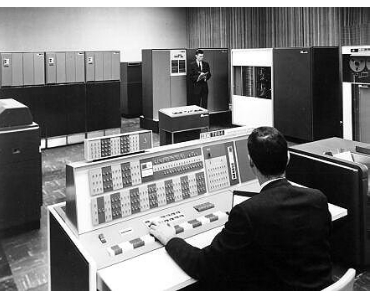
\includegraphics[width=.8\linewidth]{IBM7094.jpg}
  \end{sidecaption}
\end{figure}

D'un point de vue technique \textcite{Haggett1969} cite comme véritable point de départ dans la discipline la  démocratisation de l'accès à la ressource informatique après 1961, avec la diffusion d'une deuxième générations d'ordinateurs dans les grands centres de calculs, en partant notamment de la série IBM 7094, le CDC 3400 de Northwestern \autocite[3]{Marble1967}, des ordinateurs que l'on imagine beaucoup plus accessible et performants que la précédente série IBM 604 et 650 qui suivront (voir \href{http://www.aag.org/cs/garrison}{@Garrison}...

En nouvelle Zélande, Golledge nous indique qu'IBM semble précéder de peu la formation des pionniers [94]\autocite{Bailly2000}, et au début des années 1960 l'université de Canterbury se porte acquéreur d'un flambant neuf IBM 1620 doté de 32K de mémoire.

En suède, trois ordinateurs sont construits courant des années 50-60 :  SARA at Saab in Linköping , DASK at a Scientific Institution in Copenhagen et SMIL , University of Lund. \autocite{Persson} Carl Erik Frodberg, un ami d'enfance de Hagerstrand, fait partie avec Eric Stemme des consultants amené à échanger sur le sol Américain avec les leaders du domaine (Neumman, etc.) afin de démarrer le programme Suédois. SMIL (Siffermaskinen i Lund) à l'université de LUND est capable de compiler de l'Algol, et c'est probablement sur celui là que Hägerstrand ou Frödberg a pu faire tourner ses premier programmes. En 1969, un Univac 1108 est acheté pour faire suite à SMIL. \hl{A compléter éventuellement par la suite}

En France, il faudra attendre les années 1970 pour que l'université Paris 1, centre de référence pour les géographes pionnier quantitativistes, se dote d'une terminal Philips en contact avec le calculateur d'Orsay.

En réalité, malgré l'apparition début des années 1970 des premier postes informatique individuels, l'expression de la simulation de modèle à la fin des années 1960 est toujours limité par des problématiques humaines, techniques très fortes \autocite{Haggett1969} \autocite[387]{Marble1972}, dont on peut constater dans les ouvrages inter-disciplinaires vu dans la section précédente, qu'elle ne touche pas en réalité que la géographie \autocite{Guetzkow1972}.

Cette période ou les compétences informatiques nécessaires à la programmation se font encore très rare, les langages de programmation multiples et peu stable, le matériel coûteux et peu disponible, des packages de programmes disponible dans les universités sont quand même peu à peu publiés. Des pionniers comme Marble ou Tobler mettent à disposition courant des années 1960 différente routines informatique en libre accès \autocite{Haggett1969}  (\textcite[3]{Marble1967} parle de 150 routines développés jusqu'à 1967, cela seulement à Northwestern dans le département géographie), le premier package pour les science sociales SPSS (\foreignquote{english}{Statistical package for Social Science}) date quand à lui de 1968 \autocite{Barnes2011}, date à laquelle sort également l'ouvrage \foreignquote{english}{best-off} de Berry et Marble \foreignquote{english}{Spatial Analysis: a Reader in Statistical Geography}, qui offre une vision des derniers développements informatiques et mathématiques, et donne ainsi corps à la statistique spatiale. \hl{A modifier parcque c'est faux}

En faisant régulièrement états de leur avancements dans divers rapports ou publications, les pionniers Marble, Morril, Pits et Bowlby \autocite{Pitts1963} qui se place dans la continuité des premiers travaux relatifs aux processus de diffusion d'Hagerstrand \autocite{Hagerstrand1953, Hagerstrand1967a} donne ainsi à voir les efforts et les difficultés auquelle la petite équipe doit faire face pour améliorer les programmes, ou les adapter à des problématique différentes.

Sur un tout autre front, celui du développement des \textit{large scale models} \autocite[8]{Batty1976} \autocite[11]{Batty1994}, les universitaires géographes paraissent en réalité plus spectateurs qu'acteurs, et semblent si on en croit \textcite{Haggett1969} attendre beaucoup des retombées de ces grands programmes qui dispose de moyens humains et économiques importants pour développer des programmes et collecter des données.

Si le requiem de \textcite{Lee1973} a bien eu un effet non négligeable sur la construction et la publication de tel modèles du coté des planifieurs \footnote{Seulement trois modèles seront publiés dans le même journal à la suite de cet article ...}, force est de constater que la construction de simulation pour la théorie urbaine ne disparaît pas dans cette période \autocite[11-12]{Batty1994}, et s'appuie au contraire sur l'apprentissage de ses échecs pour se réinventer dans les années qui suivent. A ce titre, \textcite{Harris1994} soulève dans une relecture très critique de l'article de Lee, l'obfuscation ou la méconnaissance de l'auteur vis à vis des débats qui agite déjà depuis plusieurs années la simulation de modèle urbains \autocite{Wilson1970, Orcutt1957, Harris1968}. Ce faisant, Harris accuse Lee d'enfoncer des portes ouvertes et de porter des accusation que certains jugeront par la suite prématurés vis à vis du préjudice subit, touchant à coeur une discipline encore bien jeune et en phase d'apprentissage, d'à peine une décennie. \autocite[p11]{Batty1994}.

Ce mouvement de modélisation doit faire face à l'expression de ces limitations pour se reconstruire, limitations dont on sait par avance qu'elles ne seront pas seulement levés par la seule amélioration des techniques. Ainsi pour \autocite[11]{Batty1976}, plus importants que tout les autres problèmes, c'est la révélation dans l'observation de cette richesse et de cette complexité d'interactions des facteurs causaux à l’œuvre dans l'évolution et la structuration des phénomènes urbains qui va le plus impacter sur la réévaluation des formes de modélisation. \footnote{Une analyse qu'il reprend dans son article de 2001 \autocite{Batty2001}, axé essentiellement autour de l'évolution de l'articulation des mécanismes internes aux modèles et aux répercussions que cela entraine dans la construction et la validation des modèles. \hl{Une problématique qui sera reprise par la suite}}

D'une part l'emploie de théories trop simplistes induit indirectement la nécessité d'un retour à une démarche inductiviste plus exploratoire \footnote{On notera par exemple le témoignage de \autocite{Boyce1988} lorsqu'il dit à propos des chercheurs engagés dans cette voie \foreignquote{english}{Some, including myself, turned to more empirically oriented research activities, perhaps in the hope of strengthening the foundation of future models}}, jusque là mise de coté. 

D'autre part, une voie d'évolution possible des modèle vient des travaux existant réalisés par le milieu universitaire. Bien que peu sollicité \autocite[9]{Batty1994} pour la construction de ces modèles qui sont avant tout conçu dans le cadre d'une stratégie efficace de plannification, et ou l'efficacité l'emporte le plus souvent sur la curiosité scientifique, celui n'est pas en reste de ses propres travaux. Ainsi différentes équipes de développements sont déjà bien identifiées dans la communauté universitaire des économistes comme \textcite{Orcutt1960} et son premier modèle micro \foreignquote{english}{bottom-up} développé aux Urban Institute, les démographes sur les modèles de migrations inspirés des travaux d'Orcutt comme REPSIM, puis POPSIM; et enfin l'apport de \textcite{Forrester1961} sur l'optimisation industrielle, une des branche opérationnelle d'inspiration la plus directe du projet systémique au début des années 1960 \autocite{Cohen1961} \autocite[911]{Shubik1960b}.

% et Hagerstrand ? 
La \enquote{micro simulation} initié par Orcutt, qui semble effectivement passer outre l'extinction annoncé par Lee en 1973, rencontre même un certain succès durant toute les années 1970 comme en témoigne la mise en place de nombreux programme nationaux au début des années 1980. \autocite{Baroni2007} Une réponse à cette survie peut être avancé dans le positionnement innovant d'Orcutt pour face aux résultats décevant des \textit{Large Scale Models} de son époque, opérant pour la plupart à un niveau macro et fournissant des résultats hautement aggrégés difficile à exploiter dans un cadre prédictif, et finalement peu représentatif de la diversité des systèmes économiques \autocite{Birkin2012} \autocite{Baroni2007}. Si les critiques de Lee peuvent pour la plupart être mobilisé pour critiquer les modèle issue de la micro-simulation (complexités des modèles, absence d'objectifs clairement posés, volume des données à mobiliser, complexité des calculs, coût de construction, absence de résultats, etc.), il n'en reste pas moins que la proposition d'Orcutt introduit avec une approche plus \textit{bottom-up} une dimension explicative absente jusque là. En répondant à l'observation de Lee sur l'absence d'extraction de connaissance micro quelque soit la complexité injecté dans les modèles macro, Orcutt ouvre d'une certaine façon la voie à des développements théoriques beaucoup plus riche que ne le permettait à l'époque les seuls modèles Macro, faisant ainsi de son modèle un instrument pour \foreignquote{english}{consolidating past, present, and future research efforts of many individuals in varied areas of economics and sociology into one effective and meaningful model; an instrument for combining survey and theoretical results obtained on the micro-level into an all-embracing system useful for prediction, control, experimentation, and analysis on the aggregate level} \autocite[122]{Cohen1961}.

D'un autre coté, cette micro-simulation telle que théorisé par Hägerstrand dans sa version spatiale ou par Orcutt dans sa version économique, va étonnamment et cela pendant plusieurs années rester un courant ayant peu d'impact sur le développement des modèle urbains en économie spatiale \autocite[5]{Sanders2006}, et cela malgré plusieurs appels d'un coté \autocite{Hagerstrand1970} ou de l'autre \autocite[5]{Isard1998}. De façon indépendante et dans un univers somme toute limités par de forte contrainte techniques et financières, ces travaux vont toutefois dans leur lentes et multiples convergences donner naissance autant à des modèles universitaires que des programmes nationaux (DYNASIM et CORSIM pour Orcutt aux Etats-Unis, SVERIGE en suède, etc.). Pour finir cette parenthèse sur la micro simulation sur une petite transgression temporelle, si peu de modèles existent encore dans les années 1990, plusieurs publications récentes font état d'un inversion de la tendance ces 20 dernières années \autocite{Lenormand2013}, avec une augmentation (et une diversification ? ) croissante des modèles, sûrement liés à des capacités de développements informatiques plus importants, tant du point de vue des données, que de la puissance d’exécution qui admet l'importance croissante du parallélisme, idéale pour simuler des entités individuelles. \autocite[5]{Sanders2006} \autocite{Lenormand2013}

De plus cette crise qui on l'a vu touche avant tout les institut de planification couvert par la RAND va fournir \textit{post mortem} le terreau enrichissant nécessaire à la transformation d'une discipline dont le rayonnement dans la communauté scientifique à l'international ne va aller qu'en s'amplifiant après 1970 (voir la carte des foyers ou sont pratiqués la modélisation urbaines en 1980-90 dans \autocite{Wegener1994}).

Autre pistes encore de développement pour ces universitaires, les retombées de certains modèles produit par en partenariat avec la RAND ayant fourni de bon résultats, comme celui de Lowry \autocite {Lowry1964}, vont fournir la base de nouveaux travaux mettant en perspective l'influence ou les progrès d'autres courants disciplinaires en contact avec la géographie. 

Ainsi la \foreignquote{english}{social physics} de \autocite{Wilson1970} est considéré comme un moment important dans le renouveau des modèles urbains \autocite{Griffith2010}, de la même façon que le projet systémique des cybernéticiens d'abord et de Bertalanffy ensuite, qui contient dans son expression tout les outils conceptuels et opérationnels permettant la modélisation et l'étude d'un objet au travers de ses interactions complexes, comme la ville \autocite{Forrester1969} \autocite[11]{Batty1976, Batty2001} mais aussi plus généralement tout autre objet géographique \autocite[27-28]{Pumain2003} \footnote{ Pumain liste au moins trois intérêts qui découle de cette phase d'acquisition du projet systémique : a) le dépassement de l'opposition idiographique et nomothétique, b) l'histoire et les particularités des entités géographiques vues comme expression originale de trajectoires et de bifurcations, c) le dépassement de la rigidité des trajectoires biographiques historiques par l'emploi des simulations}

Mais il serait réducteur de parler de ce renouveau qui touche une catégorie de modèle bien spécifique, les modèles urbains, sans évoquer également les travaux précurseurs d'une autre branche de développement universitaire, qui semble intégrer là aussi tout à la fois les influences du courant néo-positivistes que les influences systémiques. %% FIXME %%

Si les années 1970 souffre moins de cette problématique technique, du fait en partie de la simplification des modèles, les problèmes relatifs à la validation des modèles restent eux tout à fait d'actualités. Un témoignage recueilli dans un échange de mail en 2013 avec Marble, interrogé au sujet de la suite des problématiques de validation des modèles de simulation détaillés dans son article de 1972 \autocite{Marble1972}, conforte ce point de vue : \foreignquote{english}{As I recall, the situation in the 1980's had not changed very much. Simulation in human geography did not last long. Much of this was the result of a lack of computer capacity. Simply replicating Hagerstrand's diffusion model proved difficult and our attempt to inject a more explicit temporal element just would not work due to the computational load.}

\hl{Un témoignage à mettre en relation avec les tentatives des géographes Français des années 1980, ou les problématiques de validation sur des modèles, opérant pourtant sur des populations agrégés, restent largement limités par des problématiques de calculs, la nécessité d'intermédiaire humain et technique. Les analyses statistiques doivent être adapté à la dimension spatiale,} % A détailler un peu %

%%FIXME : A MODIFIER POUR COLLER AVEC LE PARAGRAPHE PRÉCÉDENT %%


%Paradoxalement il donne aussi à voir les limites des approches proposés pour létude de l'homme dans son environnement, et offre ainsi le matériel idéal pour appuyer la formulation critique des géographes radicaux marxiste, un mouvement qui s'amplifie dès le début des années 1970 en parallèle avec la conjoncture politique nationale et mondiale. \autocite{Golledge2006}


Nombres de problèmes vont par la suite se débloquer dans le courant des années 1970 en géographie.

% Ajouter reférence denise complexité, qui permet de faire le pivot dans l'argumentation, sur systémiquer qui permet de dépasser idiographique vs nomothétique (à vérifier dans le texte)

Le mouvement du professeur Orcutt \autocite{Orcutt1957}, mais aussi celui de Forrester \autocite{Forrester1961, Forrester1969} vont par la suite amener chacun à leur manière une nouvelle dimension explicative et l'ajout d'une dimension temporelle dynamique plus à même d'aborder cette complexité qui fait largement défaut aux théories actuelles. \autocite[p295]{Batty1976}

Ainsi les progrès fulgurants de l'informatique, l'apparition de nouveaux langages exclusivement orienté pour la simulation comme Dynamo, la prise de conscience tout au long des années 1960-70 des défaut de cette première génération de modèles, et les changement d'objectifs de la discipline \autocite[12]{Batty1994} \autocite{Boyce1988} autorisent (voire recommandent) la formation de nouveaux modèle. Ceux ci sont concus comme plus parcimonieux, autorisant les démonstrations plus abstraites \autocite{Forrester1969}, plus orienté vers la compréhension des mécanismes à l’œuvre que sur la prédiction (un retour sur les modèles théoriques est opérés), intégrant plus facilement l'hétérogénéité dans la nature des dynamique (rétro-action, non linéarité) des processus \autocite{Forrester1969, Wilson1970, Allen1978}, et ouvert à l'intégration d'autres dimensions explicatives à l'oeuvre dans la formation des processus, comme ceux déjà exploré l'individu et le temps \autocite{Hagerstrand1967a,Orcutt1957,Forrester1961}. En lisant les articles de Pred, d'Olsson \autocite{Olsson1969,Olsson1970}, de Curry, on percoit chez les nouveaux économistes spatiaux cette volonté de changement, avec la reintroduction de la stochasticité et des modèles probabilistes, l'intégration du temps dans les modèles, mais aussi les causalités multiples.

% PLUSIEURS points développement méthodologiques accompagnant renouvellement théoriques accompagnant nouvelle géographie : Hagerstrand , Orcutt -> causalité + individualisme méthodologique,  Forrester -> complexité
% Hagerstrand premiere utilisation montecarlo en science sociale, vient a Washington et rencontre Morril... qui pour Benko Stromayer marque troisieme theme dominant le bouleversement quantitatif) Gould2004

% simulation permet de développer cette causalité ...
% Systeme dynamique, non linéarité, permet avancée fondamentale dans les questionnements, révélateur aussi de l'apport des techniques / méthodologies...
% Basculement vers explicatif !

Malgré la levée d'un certain nombre de contraintes, et le nouveau souffle porté par la complexité et ses supports, la problématique de la validation des modèles restent pregnante, voire parfois indépassables du point de vue technique.  \autocite[296]{Batty1976} 

Le type de formalisation mathématique qu'ils utilisent pour engendrer une dynamique leur permet de provoquer des modifications qualitatives de la structure spatiale des villes. \autocite{pumain1984} pour appuyer autoorganisation ..

\section{De la constance des problématiques dans le temps}
\label{sec:constante_problematique}

Heureusement, les capacités de calcul informatique et les méthodes de modélisation multi-échelles des informations spatio-temporelles se sont bien développées, en parallèle et en réponse à ces nouveaux défis. Parmi les sciences humaines et sociales, les géographes sont aujourd'hui particulièrement présents dans l’expérimentation et la mise au point méthodologique, qu’il s’agisse des les appliquer à des données environnementales (Kanevski, Delahaye, Douvinet) ou à des problèmes de géographie urbaine (Batty, Banos, …Ruas) ou régionale (Wilson, Dauphiné, White, Engelen, Daudé) ou encore à l’analyse de réseaux (Rozenblat). 

Les systèmes complexes sont bien entendu aujourd'hui au cœur des interrogations en sciences humaines et sociales, dans la mesure où il est connu depuis très longtemps dans ces disciplines que les interactions en jeu ne sont pas linéaires \todo{ (Morin, 200 ) }  (Morin, 200 ), que des individus engagés dans des processus collectifs sont susceptibles de donner lieu à des phénomènes originaux à l’échelon macroscopique (Schelling, 1978) \todo{ (Schelling, 1978) }, et que les situations initiales ou les effets de contexte sont parfois aussi déterminants que les modalités qui règlent les échanges entre les individus, suscitant des évolutions où la \foreignquote{english}{path dependence} \todo{ (Arthur, 1994) } (Arthur, 1994) ou \enquote{enchaînement historique} joue un rôle très important, en limitant les expressions des dynamiques possibles.

Suivant une remarque emprunté à Gould \autocite[31]{Gould2004} \enquote{[...] il faut bien se rendre compte que la formulation de questions et les avancées méthodologiques sont les deux faces d'une meme piece}. Banos \autocite{Banos2013} compte jusqu'à quatre étapes majeures ou progression technologique rime avec évolution et remise en question des questionnements théoriques. Ainsi, tout comme la systémique et la formalisation mathématique avait permis la découverte des trajectoire complexes mais cohérentes des objets géographiques, soumises non plus à des rencontres locales mais à des contingence génératrice de bifurcations dans la dynamique des villes \autocite[137]{Pumain2002}, l'apport de la modélisation multi-agent des années 1990 pousse elle encore un peu plus loin la transformation. \autocite{Sanders2007}

%Avec l'apparition des modèles agents comm en géographies les nouvelle approches ouvrent de nouvelles voies à la pensée et au questionnement littéralement impensables auparavent, on peut citer par exemple la programmation déjà linéaire, qui souleve (cf Leslie Curry, aussi cité ailleur par Hagget je crois) + introduction de Gould1970 "The intellectual revolution in geography since the middle and late fifties rests upon two main supporting pillars" 

Les modèles d’agents employés en géographie ont la particularité d’avoir été développés non seulement pour des simulations d’agents individuels, par exemple pour simuler la diffusion d’épidémies dans un territoire urbain ou régional ou sur un réseau (Banos SRAS, Badariotti, Laperrière, Eubank…) ou la diffusion d’innovations (Daudé), la propagation d’incendies (Langlois), ou encore pour éclairer les choix résidentiels (Bonnefoy…) mais ont démontré l’intérêt de modélisations fondées sur des entités plus vastes (villes, régions, voire états du monde) pour examiner les possibilités d’émergence à partir de leurs interactions à des niveaux géographiques plus larges. 

%Le laboratoire Géographie-cités a été pionnier dans l’application à la géographie des systèmes multi-agents, notamment avec la série des modèles Simpop réalisés en collaboration avec des informaticiens (Bura et al., 1996, Sanders et al., 2007, Pumain, 2012) mais aussi avec des modèles d’agents développés directement avec des logiciels simplifiés comme Netlogo (Banos…). L’évolution des modèles ne se limite pas à l’emploi de logiciels mais participe plus généralement des réflexions de la communauté scientifique intéressée par les systèmes complexes. Le GDRE S4 (Simulation Spatiale pour les Sciences Sociales) a par exemple inscrit son action parmi les premiers projets de l’Institut des Systèmes Complexes de Paris-Ile-de-France (ISC-PIF) fondé par Paul Bourgine \todo{ (ref) }. L’UMR  Géographie-cités est devenue en 2011 l’antenne  de l’Institut des systèmes complexes à l’Université Paris I et acquiert du matériel pour sa propre autonomie de fonctionnement.

Toutefois, là ou on aurait pu attendre une amélioration sur les questions de la validation des modèles de simulation agents, on se rend compte qu'un certain nombre de problématiques persistent et limitent toujours la diffusion des modèles en dehors du cercle bienveillant de l'inter-disciplinarité \autocite{Richiardi2006}. Ce problème, loin d'être un isolat touchant uniquement les sciences humaines et sociales, existe dans d'autres disciplines, comme c'est le cas en écologie, où même lorsque les modèles sont publiés, l'absence de protocole pour répliquer, évaluer le modèle est courant \autocite{Grimm1999}.

A juste titre donc, l'absence de protocole pour l'évaluation des modèles est cité comme un des nombreux écueils avec lequel se bat toujours la discipline \autocite{Heath2009}, comme en témoigne les discussions réccurentes de nombreux auteurs sur un sujet dont la complexité touche à une dimension technique, que méthodologique ou philosophique. Autant d'auteurs \autocite{Richiardi2006} \autocite{Fagiolo2007} \autocite{Moss2008} \autocite{Windrum2007} \autocite{Barlas1996} \autocite{Amblard2003} \autocite{OSullivan2004} \autocite{Doran2000} \autocite{Crooks2012} \autocite{Rouchier2013} dont il faudra développer les discussions.  

Un problème qui met un peu plus en danger des communautés de chercheurs dont on sais déjà leur isolement : archéologie, sociologie \autocite{Manzo2007}, et économie \autocite{Lehtinen2007} \autocite{Richiardi2006} pour n'en citer que quelqu'une. 

cette critique récurrente de l'outil sur le plan de la scientificité, une faiblesse qui constitue toujours un danger pour la pérénité des pratiques inter-disciplinaire autour de la simulation agents \autocite[220]{Squazzoni2010}, a tel point que la communauté se dote de guides de survie pour se protéger des sceptiques. \autocite{Waldherr2013} Est ce là le seul fait d'une mauvaise communication autour de notre discipline comme le laisserait penser la lecture de ces travaux ? 

De plus ce manque de crédibilité, qui prend souvent la forme de serpent de mer \footnote{ On pensera nottament à cette fameuse question, récurrente lors des assemblées : \enquote{Avez vous validé votre modèle?} et si oui, \enquote{Quelle connaissances pouvez vous en tirer vis à vis de votre discipline ?} \autocite{Amblard2006} } opère dans un cercle vicieux où l'absence d'évaluation nourrit une perpétuel remise en question de cet outil et de sa scientificité. %% REPETITION

Cette étape de validation, l'écueil le plus important surement, est pourtant souvent évoqué comme une étape cruciale dans bon nombres de guides méthodologiques pour \enquote{la bonne construction des modèles}, qu'il soit ancien \autocite[195]{Beshers1965} \autocite{Naylor1966, Naylor1967}, récent \autocite{Amblard2006, Gilbert2008}, technique ou atechnique. 

Malheureusement, cette étape est très rarement \footnote{On soulignera à ce titre la qualité de l'ouvrage de Railsback et Grimm \autocite{Railsback2012}, les deux auteurs prenant le temps de développer ces aspects en détail avec des exemples} mis en oeuvre dans des exemples concrets \footnote{On pourra se référer à la critique cinglante de \autocite{Manzo2007a} vis à vis du guide méthologique établit récemment par \autocite{Gilbert2008}, particulièrement muet sur la question de la validation du modèle qu'il défend dans l'ouvrage... Si même les auteurs aussi cités et reconnus que Gilbert, qui ont la chance de publier pour la première fois cette méthode dans une collection aussi reconnu (\textit{Sage Quantitative Applications in the Social Sciences}), ne donne pas l'exemple, que doit on attendre des plus jeunes recrues s'essayant à cette technique ?}, et cela en partie du fait de la nature tout à fait contextuelle de cette étape, cf.\blockquote[Amblard2006]{[...] les questions pour  la validation des modèles ne devraient jamais être abordées en dehors des questions relatives à leurs usages}

Il ne serait alors pas outrancier de de tenter ici une comparaison entre la désillusion vécu courant des années 1970, et la situation tel qu'elle apparait en 2014. Car sur ce point, un regard sur l'histoire passée de la simulation dans les sciences sociales n'est pas fait pour nous rassurer, la plupart des problèmes cités comme facteurs limitants dès les années 1970 recoupent encore aujourd'hui tout ou partie de nos problèmes actuels. On pourra arguer que certaines problématiques, comme les problématiques techniques d'accès aux ordinateurs, ou aux programmes ont quasiments disparu. Certes oui, mais de nouvelles problématiques, de même nature, sont apparus, et s'avère tout autant limitantes dans le but poursuivi. La problématique de l'accès et de l'utilisation d'une puissance de calcul nécessaire et suffisantes pour l'exploration des modèles n'est ainsi qu'une translation à un niveau supérieurs de problématiques plus anciennes...

%En forte interaction, ceux ci peuvent être rapportés à au moins trois dimensions explicatives, une dimension technique, une dimension méthodologique et une dimension institutionnelle, ce qui peut être explique pourquoi ceux ci n'ont jamais pu être totalement résolus dans le cadre d'une seule politique, d'une seule projet, ou d'une seule publication : faible nombre de modèles publiés et reproductibles, absence de publication décrivant des protocoles d'évaluation de modèles et des mises en application de ces protocoles, difficulté d'accès à l'information et à la ressource technique nécessaire pour l'exploration des modèles, stratégie de publication misant sur la publication de modèles déjà finalisés mais jamais appliqués de nouveau, manque de formations adaptées ou dédiées, confrontation avec des courants disciplinaires \textit{mainstream} ignorant l'activité modélisante, etc.

%La plupart du temps, ces papiers méthodologique pointent des arguments faisant état des limitations techniques, mais il apparaît de façon assez nette que la problématique de la validation des simulations et la lutte régulière pour reconnaître le caractère « scientifique » de la simulation et son intérêt pour dégager de la connaissance semble être un argument transerval dans les différentes disciplines et dans le temps.

%En reprenant notre argumentaire pour y exposer non plus le modèle non plus dans sa dimension uniquement technique, mais dans sa dimension de construit, de nouveaux objet d'étude apparaissent.
Ce qui semble être décrit comme une immaturité dans la méthode Agents \autocite{Heath2009} se rapporte en réalité à des pratiques qui dépasse largement l'utilisation spécifique de cette technique spécifique. La simulation agents en apportant cette nouvelle et importante flexibilité dans l'expression des problématiques de recherche, a pu certainement provoquer un effet de mode menant à des dérives, un état de fait qui ne nous fera pas oublier l'enracinement d'une bonne partie des critiques qui lui sont adressés, à tort ou à raison.

Compte tenu de cette persistance des problématiques dans le temps, au delà de l'évolution des techniques, il est fait ici un choix radical. En objectivant cette \enquote{démarche scientifique de construction de modèle} pour en faire un objet d'étude à part entière, et en laissant dans un premier temps de coté les supports techniques (modèles équationels, modèles agents, etc.), il est proposé dans cette étude de se concentrer sur la problématique de validation/vérification des modèles, une étape que l'on juge déterminante au cœur de la construction du modèle. 

Un retour sur la démarche de construction des modèles en géographie s'avère nécessaire pour comprendre les éléments qui nous ont échappés dans la continuité de cette problématique qu'est la validation des modèles. En s'appuyant sur les témoignage de \autocite{Batty2001, Pumain2003} on parvient très bien à décrire ce basculement opéré à la charnière des années 1970, alors même que les géographes accède peu à peu aux concepts opérant dans le paradigme systémique \autocite{Harvey1969}, et que l'insuffisance des démarches de construction de modèles devient prégnante 

\hl{bof}

\subsection{Phase de transition des années 1970} 
\label{ssec:transition_annee70}

La section précédente traitant de la crise/renouveau de la simulation en géographie abordée cette problématique principalement du point de vue des outil, hors ces problématiques techniques et méthodologique se double d'une crise épistémologique où la \enquote{vérification} concentre nombres de critiques. 

La fin des années 1960, début des années 1970 voit l'émergence de nouveaux courants de géographie qui rentre en conflit avec les présupposés quantitativistes de la premières vague, les acteurs prônant une démarche scientifique teinté de néo-positivisme inspiré des sciences physiques subissent un front de critique \autocite[61-64]{Paterson1984}

Si il n'est pas question ici de relater l'émergence de ces différents courants, comme la géographie radicale, ou comportementale, dont la complexité de traitement dépasse largement la portée de cette thèse, il est toutefois possible de citer le contexte historique de sa formation, dans une conjecture qui dépasse la seule dimension critique envers les méthodes quantitative. Les causes de cette diversification se fait au jour de problématiques politiques (crises nationales et internationales, guerres) tout autant que théoriques (rejet des méthodes quantitatives) et méthodologique (retour de l’herméneutique).

Il est quand même utile de faire ressortir une parties de ces facteurs pour mieux observer en quoi cette crise est vécu tout autant de l'intérieur, entraînant comme on l'a déjà décrit dans la \hl{section XX} une transformation des modes de construction, que de l'extérieur des disciplines attaqués. Cette rupture épistémologique est plus l'expression d'un autre style de pensée mettant à disposition de nouveaux moyens pour l'explication. A ce titre, il me semble que le développement de la systémique, se place dans une continuité de réflexion sur les objets géographiques qui amène dans cette phase de transformation critique de la discipline à dérouler des modèles capable eux aussi de rendre compte de façon complémentaire de cette complexité des interactions entre l'homme et son milieu.

\subsubsection{Quelle réalité dans l'application de la démarche explicative néo-positiviste}
\label{sssec:realite_neopositiviste}

Les critiques sont sur plusieurs fronts, celle premièrement de la philosophie néo-positiviste comme projet réaliste pour l'explication, l'inadéquation des démarches proposés par les théoriciens géographes trop éloignés des pratiques des scientifiques, l’échec des modèles centrés sur la prédiction

\paragraph{Un état critique du débat épistémologique néo-positiviste dans les années 1960-70}

Dès 1940 Hempel, un des membres influents dans le cercle de Vienne, s'intéresse de plus près à la problématique de la \enquote{confirmation} dans le cadre du modèle hypothètico-déductif, nommé par la suite H-D confirmatif. Il va alors être le premier à s'interroger \enquote{[...] non pas sur la formulation d'un hypothèse ou d'une loi universelle à partir de cas particulier, mais sur la \textit{confirmation} d'une hypothèse ou d'une loi donnée} \autocite{Lecourt2012}. Cette démarche va connaitre rapidement plusieurs difficultés, avec l’avènement de plusieurs paradoxe bousculant les les démonstrations logiques, comme le paradoxe de Goodman, ou celui d'Hempel (Raven Paradox). Certains paradoxe seront résolus dans différentes déclinaisons du modèle H-D, mais d'autres resteront problématiques, amenant peu à peu à l'affaiblissement de l'approche cumulative empiriste. 

Dans les convergences entre faillibilisme Popperien et positivisme logique, il existe des divergences aussi forte que ne peuvent être les convergences. Ainsi à méthode H-D quasi-similaire, l'hypothético-déductivisme de Popper impose pourtant un raisonnement inverse pour la formulation des hypothèses. Il ne s'agit plus d'une formulation pour la construction incrémentale de loi ou de théorie, mais d'une formulation dont la fonction est avant tout de destabiliser une théorie ou une loi existante. Pour Popper la science avance dans une perspective critique, la théorie de la relativité d'Einstein fournissant un parfait exemple de situation ou le seul échec d'une expérimentation peut remettre en cause toute un pan de la théorie. Dans le langage de Popper, l'hypothèse devient conjecture, et la vérification est donc empreint d'un double sens : une corroboration en cas d'une confrontation positive, et une falsification en cas de confrontation négative. Avec cette particularité que lorsque la conjoncture est vérifié, celle ci est d'un apport beaucoup plus faible que dans le cas d'une vérification, du fait des nombreux paradoxe qui accable le \enquote{problèmes de l'induction}, et que Popper veut écarter définitivement du processus de démarcation entre science et non science.

Popper, rationaliste et plus proche critiques des méthodes des positivistes logiques va proposer un modèle H-D en négatif qui remet en cause complètement l'empirisme logique des positiviste logiques. Celui-çi, de nouveau compatible avec la métaphysique, ne supporte plus une logique de confirmation mais de réfutation comme moyen pour séparer science et non-science.

La méthode H-D de confirmation permet rejeter ou d'accepter des énnoncés observationels, mais elle ne constitue pas en elle même une méthode \enquote{explicative}. La méthode Deductive Nomologique (D-N) formulé par Hempel et Oppenheim’s  est en 1945 une tentative tout à fait originale pour créer une logique formelle centré sur l'explication.

\hl{Explication rapide modèle ND}

Des discussions internes et externe de ce programme néo-positiviste s'étalant sur plusieurs dizaines d'années ressortent deux modèles en définitive compatible, le modèle Hypothético Déductif H-D pour la \enquote{confirmation} de Popper et Déductif Nomologique (D-N) (connu aussi sous le nom de \foreignquote{english}{covering law}) pour \enquote{l'explication} de Hempel-Oppenheim ou encore Hempel-Popper.

Il ne s'agit pas de rentrer dans les détails des critiques qui ont étés faites à ces deux versions de modèles ici, tant elles ont été nombreuses, et sur ce sujet on pourra se rapporter aux ouvrages de \textcite{Chalmers} et \textcite[214-215]{Meyer}. On retiendra toutefois que les principaux acteurs de cette méthode, comme Hempel, le principal artisan de la méthode N-D abandonne définitivement le modèle vérificanioniste en 1950-51, et le falsificationisme en 1965, des dates qui illustrent le décalage temporel existant avec les tentatives des théoriciens comme Harvey d'adhérer à une telle démarche en 1969, alors qu'elles sont d'ores et déjà dépassés.

%Parmis les défaut principaux qui paraissent poser problème pour un usage raisonné de cette méthode dans la discipline, a) il est impossible de différencier logiquement une loi d'une simili-loi, comme cela pourrait être le cas en géographie; b) le modèle D-N n'est pas universel ; c) la complétude dans l'explication scientifique est un mythe, et même si elle était possible était universellement possible, n'est pas un gage de scientificité, et inversement; c) la symétrie entre explication et prédiction n'est pas vrai; toute prédiction n'est pas explicative et inversement; c) le modèle est linéaire, une cause entraînant un effet, peu compatible avec la complexité du monde réel; d) le processus de découverte se situe en dehors de l'analyse e) la conclusion est contenu dans les premisses ; f) l'explication est en réalité plus justification, et ne rend pas forcément compte des processus générateur

Deux choses peuvent nous intéresser particulièrement dans ces critiques. D'une part non seulement ce modèle est loin d'être universel, et ne garantie aucunement l'explication, c'est l'objet du premier paragraphe. D'autre part la remise en cause de la symétrie entre explication et prédiction car toute prédiction n'est en soit pas explicative et inversement, et fera l'objet d'un deuxième paragraphe. 

%Les faiblesses dont il sais déjà qu'elles existent : ignorance de la recherche comme activité, symétrie entre explication et prédiction, absence de découvertes autres que celle contenue dans les prémisses.

\paragraph{Les principaux instigateurs du mouvement en géographie}

Si il est clair que le positivisme logique n'est pas au fondement de la révolution quantitative \autocite{Claval2003}, l'impact de ce mouvement sur la géographie dans la décennie 1960-70 existe, ne serait ce que par la portée des théoriciens qui ont bien voulu s'en faire le porte voix, cela de façon implicite comme Bunge, ou explicite comme Harvey. La mesure de cette impact reste par contre difficile, sinon impossible à quantifier. 

La première introduction au positivisme logique chez les géographes se limite aux étudiants présents sur les bancs de l'université de Washington (Seattle) et d'Iowa \autocite[554]{Barnes2001a} \autocite[120-121]{Unwin1992}, se qui concerne aussi les étudiants en déplacements pour leurs études.

Un bon point de départ pour observer la diffusion de ces méthodes semble être l'histoire personnelle de Schaefer. Il semblerait que la communauté des géographes soit en accord \autocite[15]{Louail2010} pour désigner l'article de Fred Schaefer \autocite{Schaefer1953} comme le catalyseur des frustrations d'une génération de géographe envers les pratiques alors en cours dans leur discipline, en déclin tant d'un point de vue scientifique qu’institutionnel.

Né à Berlin, Schaefer profite d'une solide formation inter-disciplinaire en Allemagne, qu'il fuit dès lors qu'il est apparenté à un terroriste par les Nazi, du fait de ses appartenances politique. Après une courte exode en Grande-Bretagne, il s'installe aux État-Unis où il participe à la diffusion de la géographie économique Allemande, par des enseignements, mais également par le biais de traduction (Lösch). \autocite{Bunge1979}

A la lecture de son fameux article méthodologique \textit{Exceptionalism in Geography} l'influence du programme des positivistes logique est évidente. Rien de surprenant à cela, en effet Schaefer meurt en 1953, et c'est son ami proche Gustav Bergmann qui prend en charge la relecture et la publication finale dans les annales de l'AAG. \autocite[32]{Gregory1978}. Philosophe proche du cercle de Vienne et lui aussi exilé, Bergmann va enseigner la philosophie à la faculté d'Iowa dès le débuts des années 1950, tout en restant très proche et très influents auprès des jeunes géographes.\autocite[192]{Buttimer1983} Ainsi, King, Clarke, Golledge, et Johnston, sont tous passés par les bancs des université néo-zélandaises et américaines et ont ainsi joué un grand rôle dans la diffusion de la géographie quantitative mais aussi du néo-positivisme dans ce pays. King, qui dispense des cours d'analyses spatiales à Canterbury dans les années 60 est passé en 57 à Iowa, et Golledge nous dit avoir suivi les cours de Bergman lors de son séjour dans cette même université \autocite[95-96]{Bailly2000}. \footnote{Pour plus d'information sur la diffusion du néo-positivisme en Nouvellve Zélande, on pourra se référer plus spécifiquement à la thèse de \textcite{Hammond1992}}

L'impact premier de cet article de Schaefer est difficile à évaluer, car celui ci ne devient un référentiel que quelques années plus tard, une fois repris par d'autre théoriciens \autocite[32]{Gregory1978} L'ouvrage en 1962 de William Bunge, premier grand théoricien de cette \enquote{révolution quantitative}, bien que faisant une référence implicite à ce mouvement, joue un rôle important dans la diffusion de ce standard scientifique. Enseignant également à l'université de l'Iowa, celui ci va se positionner sur la meme ligne que son collègue et ami Schaefer \autocite{Goodchild2001}, et affirmer dans un article fondateur \autocite{Bunge1962} sa volonté d'une géographie avant tout nomothétique, comme les autres \enquote{sciences}. \autocite{Bunge1979} \autocite{Claval2003} \autocite[429-430]{Gregory2009}. 

Un autre point de vue plus tardif mais cette fois ci explicitement teinté de néo-positivisme est réalisé par Harvey en 1969 \autocite{Harvey1969}. Bien que le travail d'Harvey soit reconnu comme un apport bénéfique à la géographie par de nombreux relecteurs (Amadeo, Gregory, Wolpert), ce travail à la fois très dense et écris sans réel public cible en tête touche finalement une audience relativement limité, notamment du coté des étudiants, qui dispose déjà de nombreux autres ouvrages déjà connus comme référence (Gregory 1963, Chorley et Hagget 1965, Abler 1971) \autocite{Johnston2008}. \hl{numéro de page ou citation ici !}

Connu pour son exploitation de la philosophie néo-positiviste, \textit{Explanation in Geography} est le fruit d'un travail d'écriture de longue haleine, conçu avant tout comme une position de recherche, autant de présupposés prémonitoires selon \textcite[47]{Barnes2006} des critiques à venir. L'écriture de cet ouvrage est donc à remettre dans un contexte spécifique, en 1960 dans l'université provinciale de Bristol, ce qui fait plus de ce livre selon Barnes \autocite[31-36]{Barnes2006} un manifeste énergique destiné à électriser la discipline, et à motiver la modernisation des institutions d'enseignement britanniques.

L'application d'une étiquette néo-positiviste à la géographie quantitative des années 1960-70 n'est pas si évident, et une relecture plus critique de cette période permet de relever d'autres motivations, qui mettent tout autant en défaut le discours globalisant des théoriciens comme Harvey, que les discours critiques des géographes radicaux rejetant en bloc toute les approches quantitatives.

\paragraph{Une étiquette néo-positiviste critiqué et critiquable}

De lecture difficile car très abstrait et mathématique, l'ouvrage d'Harvey constitue une tentative intéressante d'introduction de l'épistémologie des sciences au géographe bien qu'il reste avant tout motivé par la description d'une \enquote{démarche scientifique idéale} plus que d'une lecture rigide de l'orthodoxie prôné par les positivistes logiques. Écrit semble t il dans un certain isolement vis à vis du monde, on comprend mieux pourquoi Harvey choisit dans son ouvrage de défendre une démarche scientifique qui sur la fin des années 1960 est déjà très largement critiqué, voire abandonné par les autres philosophes des sciences. \autocite[57]{Harvey1969} \autocite[147]{Ouelbani2006}. Mais en prenant cette posture, Harvey s'expose tout autant au foudres des philosophes, pour qui une attitude plus laxiste pourrait trahir la logique des démonstrations en place, que les foudres des géographes tout à fait enclin à la pratique d'autres types de démarches scientifique.

En 1972, l'ouvrage \textit{Explanation in Geography} est très vivement attaqué par une critique longue et argumenté de \textcite{Gale1972} dans le très sérieux journal \textit{Geographical Analysis} Bien qu'Harvey présente d'autres démarches explicatives dans son ouvrage, et présente une lecture quoique superficielle, mais lucide des critiques énoncées sur la démarche néo-positiviste, il choisit quand même un alignement sur l'explication nomologique-déductive, moyennant le soulagement de certaines contraintes \autocite[39-40]{Paterson1984}. Ce qui en fait selon \textcite{Gale1972} un ouvrage propice aux débats, mais d'un autre usage limités, car cette posture de l'auteur, fluctuant entre entre examen pratique et application rigide de ce logicisme philosophique introduit de nombreux paradoxes dans l'argumentation de l'auteur.

Outre le fait que l'application de cette démarche est d'emblée qualifié comme un idéal \footnote{C'est aussi l'avis d'Hempel que de penser sa méthode comme un idéal \autocite{Besse2000}} atteignable plus que d'une réalité dérivées des pratiques, il est encore plus paradoxal de voir l'auteur défendre un modèle de démarche scientifique analytique, réductionniste, usant d'une causalité linéaire totalement incompatible avec la vision du géographe, pourtant convaincu de l'éminente complexité des processus dans le temps sous-jacente à l'établissement des régularités spatiales observés et de leurs importances dans l'explication. \autocite[57-58]{Paterson1984}

Autre paradoxe, alors que la seule \enquote{loi} est censé piloter l’expérimentation dans cette démarche nomologique-déductive, Harvey admet toutefois la nécessité \enquote{d'une amorce} empirico-déductive, qui reste un élément important de cette révolution quantitative, ne serait ce que parce que la géographie ne possède jusque là, il est vrai, que de loi d'emprunts \autocite[41-42]{Harvey1969}. 

De plus, Hempel et Popper se retrouve tout deux pour affirmer leur opposition à toute \enquote{logique de la découverte}. La seule méthode valide pour faire le tri parmi l'infinité de faits disponible doit se faire par la corroboration ou la réfutation d'une inférence déductive. La formulation de l'hypothèse se fait donc \textit{a priori}, par généralisation accidentelle, ou par intuition, ce qui rend toute logique de la découverte externe au processus objectif scientifique et renvoie cette problématique à la psychologie.

\hl{détail des autres contraintes si il y'en a}

Ce faisant il construit une deuxième démarche qui reconnaît le rôle a priori des théories sur les données, qu'il oppose à la démarche classique inductive Baconienne. Le \enquote{problème de l'induction} étant ce qu'il est, irrésolu, l'inférence statistique n'est permis que dans un cadre formel orienté vers la déduction, pour la corroboration ou la réfutation d'une conjecture. Hors non seulement il est d'ores et déjà admis que les théories ne sont que des objets de travail, et donc sont susceptible de mentir tout autant que les observations, mais l'utilisation des méthodes statistiques descriptives, multi-variés comme la régression multiple, les analyses factorielles, les statistiques spatiales dans une démarche empirico-inductive joue évidemment un grand rôle dans la capacité des scientifiques à mobiliser des modèles permettant de comprendre la complexité des masses de données. Même si les problème d'autocorrélation spatiale, associé au \enquote{problème de l'induction} limite effectivement la portée des généralisations qui peuvent être faites, cela n’empêche absolument pas son utilisation dans le cadre réaliste des pratiques scientifiques, et cela on imagine durant tout le processus de construction des modèles.

Ce constat est appuyé par les travaux de \textcite{Barnes1996, Barnes2001} qui non seulement affirme le fait que bien des acteurs de la première vague théoriques semble ne jamais avoir rencontré de positiviste \footnote{Morrill1993 citation à récupérer}, mais que les principaux producteurs de ce mouvement ne sont pas non plus des grand adepte d'une application stricte de la \foreignquote{english}{scientific method} aux sciences sociales, à commencer par Bergman lui même ! \footnote{Dans le recueil de texte biographique \textit{Mémoires de Géographes} \textcite[96]{Bailly2000}, Golledge revient sur les propos de Bergman : \enquote{Bergman soulignait la différence entre ce qu'il appelait alors la science pure et la science sociale. C'était le premier à admettre que l'utilisation des procédés logiques positivistes dans la science sociale pourrait se révéler extrêmement improductive.} } 

\paragraph{Un échec qui ne doit pas masque la réalité des transformation}

La problématique des modèles \enquote{a priori} défendu également par Harvey peut être en partie retrouvé dans les critiques qui sont opposés aux ouvrages et aux projets inspirés par cette démarche néo-positiviste.

Un échec retentissant qui alimente la critique des opposants non quantitativistes, souvent privé de crédit, est sûrement l'écho \autocite{Lee1973} des résultats médiocre d'une décennie de modélisation piloté par les instituts de planification, fort coûteuse, appliqués aux systèmes urbains. Entre 1958-1968 aux États-Unis, un grand nombres de modèles théorique \autocite[7-9]{Batty1979} dérivés des modèles de l'économie spatiale naissante sont utilisés \textit{a priori} sur de larges corpus de données, et cela à des fins de prédictions plus que d'explication. Il faudra attendre plusieurs années par la suite pour que renaissent sous cette appellation des \textit{large-scale models} un tout autre programme de modélisation \autocite{Boyce1988}.

Quel exemple plus marquant peut on trouver pour démontrer que la prédiction de systèmes aussi complexe que les systèmes urbains et par extension sociaux n'est pas compatible avec une démarche de construction des connaissances qui met sur pied d'égalité prédiction et explication ? (le fameux \enquote{Expliquer c'est prédire} de Popper). La dérive de cette vision néo-positiviste de la modélisation vers une forme d'instrumentalisme ne s’intéresse pas plus ici au mode de production des phénomènes (le Pourquoi ?) \autocite[41]{Gregory1978}, les seuls pourtant à pouvoir donner une certaine intelligibilité aux lois que l'on utilise. \autocite[14-15]{Besse2000}

Dans la branche des modèles universitaires le livre \foreignquote{english}{models in geography} de Chorley et Haggett encense mais cristallise aussi \textcite{Golledge2006} tout autant la fin que le début d'un nouveau cycle. Le peu de résultats (quelles nouvelles lois spatiales ?) apportés par des modèles théoriques aux hypothèses (volontairement ou involontairement) simplifiantes (comportement optimiseur des individus sur le plan spatial et temporel, modèle déterministe, agrégé et peu explicatif, fonction d'utilités, population et environnement uniforme, etc.) dont on a imaginé qu'il pourrait à un moment se substituer à la réalité, ou amener de l'explication par la prédiction \autocite[41]{Gregory1978} entraîne une large frange de géographes à critiquer dès le début des années 1970 ce type de modèle.

\hl{Pointer vers le fait que la validation à cette époque ne jure que par les goodness of fit, cf historique déjà réalisé pointant vers vision de Naylor, largement dominante et tiré de l'enginérie}

En s'appuyant sur cet état de fait, on peut mobiliser l'argumentaire de \autocite{Wilson1972} comme l'avait fait \autocite{Gregory1978} pour mettre en difficulté l'argumentaire d'Harvey. Celui ci voit bien cette dualité qui existe entre les deux courants majoritaires de modélisation, avec d'une coté cette géographie théorique issue de la branche \foreignquote{english}{Models in Geography} qui manque de données pour tester ces hypothèses, s'avère limité dans son expression opérationnelle (les modèles micro trop complexe, la validation et la calibration encore difficile), et porte selon lui encore trop l'emphase sur l'induction statistique et pas assez sur la démarche hypothético-déductive pour former des modèle \footnote{Modèle est ici synonyme pour lui de théorie} ; et à l'inverse opposé la branche instigatrice des \textit{large scale models} qui fait (trop) usage des dernières techniques, dispose de large données, mais s'avère incapable du moindre résultats car mal équipés en terme de théorie, guidés par des objectifs divergents, où la prédiction est souvent le résultat d'un \enquote{camouflage} usant des \enquote{Goodness Of Fit} de l'économie \autocite[10]{Batty1994}.

On peut ne pas être d'accord avec ce que dit Wilson par ailleurs dans cette article, mais il fait ici figure de précurseur dans sa volonté de lié les deux approches, tant il semble bien conscient que la réussite de la démarche de construction des connaissances en géographie tient avant tout de la complémentarité entre cette approche inductive et déductive.

Mais nous aurions tort de nous arrêter dans cette analyse, et rejeter comme nombres d'auteurs l'ont fait tout approche quantitative, en l'associant à tort à cette démarche néo-positiviste, une association qui on l'a vue, s'avère plus complexe, sinon erronée.

L'échec de l'internationalisation de cette épistémologie est particulièrement marqué en Suède, et dont Hägerstrand, de tradition humaniste et transdisciplinaire \autocite{Bailly2000} passe au travers des critiques car il a prouvé par ses modèles et ses outils intégrant l'homme dans l'environnement qu'il était volontaire dans la construction d'un cadre explicatif plus riche et complexe que celle proposés par les macro-économistes. \hl{cf l'article belge cybergéo}

Autre échec notable de cette épistémologie est sa non-diffusion en France courant des années 1970. En effet, Claval note qu'elle provoque au regard de l'épistémologie post-vidalienne existante un certain rejet.. \hl{retrouver la ref}. Le débat épistémologique intéresse certes, mais selon lui les géographes français sont alors bien trop occupé alors à intégrer les fascinantes et toutes dernières techniques quantitatives pour qu'une synthèse voit le jour sur le sujet.\autocite[27-29]{Claval2003}

Des théoriciens comme Bunge, ou Harvey rejoignent dans le courant des années suivantes la fronde d'une géographie radicale émergente. Ainsi \textcite[30]{Johnston2008} et \textcite[37]{Barnes2005} nous indique pour Harvey ira jusqu'à critiquer en partie ses propres travaux, à plusieurs reprises, dans la préface du livre, dans une réponse à son principal critique \textcite{Gale1972} et dans son nouveau livre en 1973 \autocite{Harvey1972} \autocite[166-168]{Gould2004}. Ces revirements, en partie on l'imagine pour des raisons politiques, ne doit pas faire oublier que le socle de la révolution quantitative ne repose pas que sur des individualités théorique, mais aussi sur une mise à disposition massive de nouveaux outils mathématique et statistique dont l'utilisation est tout à fait neutre politiquement \autocite{Sheppard2001}, et dont la libre utilisation dans des procédures de déduction, ou d'induction tient plus de la question posé que d'une démarche imposée. \autocite{Lena2000}

\textcite{Sheppard2001}, toujours en lutte dans les années 2000 pour gommer ce débat stérile entre qualitativiste et quantitativiste géographes, argumente en la faveur d'un langage mathématique, anthropomorphe, lui aussi vivant et amené à évoluer avec le temps. 

Le sursaut et la transformation déjà étudié dans la section \ref{ssec:crise_mutation} montre que la discipline n'a pas attendu le revirements des théoriciens néo-positivistes, ou les critiques d'une géographie radicale pour remettre en question et rebondir du fait de ses propres échecs. L'évolution des mathématiques et de l'informatique permet ce dépassement, et cela au travers d'un cadre d'analyse systémique qui offre les concepts nécessaires pour sinon résoudre, au moins admettre un premier dessin de cette complexité \autocite{Dauphine2003}, avec à la clef un effet libérateur en géographie pour bien des raisons évoqués par \textcite[27-28]{Pumain2003}

%Intéressante aussi, la lecture du \enquote{manifeste} \autocite[31]{Barnes2006} d'Harvey donne à voir cette tension entre ce qui est pour lui la démarche dominante des années 1960-70, et l'ouverture vers un autre paradigme prometteur, celui de la systémique, selon lui encore peu repris et opérationalisé par les géographes, et cela malgré l'appel de plusieurs personnalités comme Berry, Chorley, Haggett. 

%Sachant que la démarche explicative néo-positiviste proposé par Schaefer, Harvey et les autres théoriciens tient plus de l'expression d'un idéal que d'une réalité pratique, la posture nomologique sous-jacente reste quand à elle une volonté forte qui motive toujours la transformation de la discipline.  FIXME conclusion modérant les propos de rejet du courant comme principal porteur ?

\subsubsection{L'intégration progressive et naturelle du projet systémique} 
\label{sssec:progressive_systemique}

\textcite{Barnes1996} produit une contre-narration intéressante sur des acteurs majeurs dans la formation de la révolution quantitative, comme Isard, Bunge, Warntz, Haggett; et prend ainsi le contre-pied de l'analyse classique plaçant la nouvelle géographie sous la seule coupe d'un néo-positivisme qui serait omniprésent. 

Encore dans une phase de découverte à la fin des années 60 si on en croit \textcite{Harvey1969}, la démarche systémique a déjà pourtant bien infiltré la géographie par le biais de porteurs dont le flambeau semble tout autant explicite qu'implicite à ses développement. Porteurs dont il n'est pas difficile de faire remonter la filiation dans l'héritage des grands mouvements inter-disciplinaire systémiques du début du XXième siècle, la Cybernétique de Wierner, et parallèlement le programme biologique organiciste de Bertalanffy, qui deviendra par la suite le projet beaucoup plus vaste de GST. \footnote{Sur ce sujet on trouvera dans l'annexe suivante un historique beaucoup plus détaillé de ce mouvement.} 

Si Bertalanffy fut marqué par le néo-positivisme à une période de son étude \footnote{Fait étonnant Victor Kraft est un géographe, philosophe proche du cercle Viennois, mais tenant d'un point de vue original rapport à ce courant. Celui forme des géographes très tôt en allemagne à des méthodologies quantitative (1929). En 1926, Bertalanffy proche du milieu viennois à ce moment, emprunte à celui ci en 1926 la méthode hypothético-déductive \autocite[342]{Pouvreau2013}. Une boucle intéressante semble alors se former entre i) Kraft dont la formation est inspiré par Pleck, un professeur allemand inspiré de la méthode déductive de Davis, ii) Kraft indirectement amené à participer au débat Schaefer-Hartshorne du fait de son travail ainsi cité, et iii) le fait que Bertalanffy va ensuite nourrir les travaux de Chorley qui prend la suite des études de Davis en géomorphologie...}, celui ci subit par la suite de très violente critiques de la part de plusieurs membres, en Allemagne, puis aux états-unis, marquant un profond désaccord qui ira en grandissant par la suite \autocite[26-27]{Pouvreau2006}. Il me parait important ici de noter dans quelle position surprenante se trouve la géographie et les géographes lorsque ceux ci appellent à la fois à l'application d'une démarche HD/ND, et leur volonté d'aller vers une démarche systémique, tant les deux système semblent s'opposer en réalité sur plusieurs points, ce qui rend leur cohabitation de toute façon relativement peu probable : approche analytique réductionniste contre holisme, causalité linéaire contre causalité multiple, etc. 

La posture nomologique des géographes, en remettant au centre de son projet scientifique les modèles et la modélisation, a réactivé dans sa révolution ce besoin non pas tant inventer des loi spatiale \foreignquote{latin}{ex nihilo}, car comme on l'a vu il s'agit d'un exercice qui a montré ses limites, mais plutôt extraire ou reconstruire en partant de ces fondements historiques la part de géographie propre à ces isomorphismes afin d'établir plus explicitement ces \enquote{loi} qui lui font défaut.

Cette diffusion du projet systémique dans la géographie semblent s'être fait en deux temps partiellement superposés, ce qui rend la mise en avant d'une seule et unique \enquote{rupture} difficile. De façon grossière, on peut se risquer à un découpage en deux phases. Si la première phase semble plus porter l'emphase sur la modélisation et le débat autour d'isomorphismes du fait de passeurs entre disciplines, la deuxième phase plus explicite d'acquisition d'une partie du projet systémique semble quand à elle généraliser ce projet de récolte d'isomorphisme, et mobilise à l'instar des sciences physiques des outils qui bouleverse notre façon d'aborder la construction des modèles en géographie. Si la première phase introduit l'idée, la deuxième semble trouver les moyens de l’opérationnaliser.

\subsubsection{Premiers passeurs et premier débats au cœur de la nouvelle posture nomologique}

Pour illustrer ce fameux thème de Norbert Elias \autocite[31-33]{Delmotte2010} \textcite{Elias1991} sur l'Homme illustre, comme produit conjoncturel des interrelation qui le porte au sommet d'une dynamique collective, on pourra citer les travaux qui mène à la bien connu loi rang taille de Zipf-Auerbach, en filiation directe avec cette dynamique de fond à la convergence des grands mouvement inter-disciplinaire et des nouveaux enseignements tirés des avancées physique de la thermodynamique du début du XX ème siècle.

Plus qu'une application directe souvent impossible, voire non souhaitable, ces isomorphismes semblent avant tout agir comme catalyseur dans la transformation d'une discipline marqué d'abord par cette impression d'absence de loi. Ainsi le cas de la distribution des tailles de villes, qui se rapportent tout autant à la théorie des lieux centraux que de la loi rang-taille, est exemplaire des débats qui vont se structurer autour des modalités d'application de ces isomorphismes, et des résultats qu'il est possible d'en tirer d'un point de vue thématique. 

L'interrogation sur la capacité du vivant \enquote{à remonter} l'entropie qui saisit la physique du début du XXème siècle amène celui ci a proposer en 1910 le concept d'\enquote{ectropie}; préfigurant ainsi les débat à venir sur cette thématique dans les années qui suivent (néguentropie de Schrödinger en 1945, second principe de la théorie organismique de Bertalanffy en 1929 \autocite[475]{Pouvreau2013}, etc.) \autocite[80]{Pouvreau2013}. Physicaliste avant tout \autocite[87]{Pouvreau2013}, Auerbac est convaincu que le progrès en biologie ne viendra que de l'explication entièrement physique des phénomènes biologiques, une vision réductionniste de la biologie qui sera largement débattu par la suite dans la thèse de Bertalanffy. Toutefois, et sur un tout autre sujet se rapportant à la physique, c'est lui qui s’intéresse en premier à l'application sur des villes de l'effet d'inégalité soulevé par Pareto dans les population.\autocite[94]{Rosser2011} Il donne naissance à la loi Rank-Taille qui montre que le produit de la population par le rang de la ville dans la hiérarchie est une constante. Une analyse repris et développé par Zipf dans une étude lexicologique à vocation universalisante, cette fois ci appliqué sur les villes, ce qui explique entre autre la confusion dans l’historique de l’appellation.

Autre exemple d'isomorphisme catalyseur des débat, on citera entre autres sur l'adaptation du modèle gravitationnel au modèle de migration de population. Sur les travaux initiaux des géographes Ravenstein (1885) et Levasseur (1889), puis l'économiste Reilly (1929), se greffent les travaux de Warntz (géographe) et Stewart (physiciens). Déjà connu des géographes par sa publication de 1947 qui pose l'isomorphisme entre population et gravité, Stewart fait probablement naitre très rapidement une certaine curiosité chez les pionniers. Ullman s'avère par exemple être un fin lecteur \autocite[61]{Glick1988} et \href{http://nwda.orbiscascade.org/ark:/80444/xv01385}{@Correspondant} de Stewart. Warntz de son coté est un géographe qui plonge dès le départ dans l'inter-disciplinarité. Financé par l'ONR il est présent à l'AGS (American Social Geography), au département de science régionale de Pennsylvania's, et dans le département d'astro-physique de Princeton où il est amené à collaborer régulièrement avec Stewart, avec qui il \href{http://rmc.library.cornell.edu/EAD/htmldocs/RMM04392.html}{@Correspond} aussi après guerre. \autocite{Barnes2006}. 

Dans les deux cas il est intéressant de noter le basculement manifeste entre application du modèle \foreignquote{latin}{a priori} sur les données, et la prise de conscience dans un long débat qui s'ensuit sur la faible capacité explicative de ces analogies, avec la nécessité d'adapter ces formulations à la discipline géographiques. 

Pour un historique beaucoup plus détaillé des débats qui ont animé (et anime encore aujourd'hui) la communauté autour de la loi de Zipf-Auerbach, on pourra notamment se référer à \textcite{Pumain1982}, et pour les modèles gravitationels à la thèse de ... \hl{A ajouter}

%Mais la recherche du meilleur modèle, ou du meilleur paramétrage de modèles mathématique pour ajuster les données s'avère rapidement inutile et décevant - quand il n'est pas en plus empreint d'idéologie - tant l'apport d'un point de vue explicatif est faible. Sur ce sujet \autocite[37]{Pumain1982} cite Tinbergen qui en 1968 affirme \enquote{qu'aucune explication scientifique digne de ce nom n'a été avancée jusqu'ici} 
% FIXME A deplacer dans le changement des années 1970

Par sa multi-formation de mathématicien, de chimiste et statisticien, et son parcours atypique Alfred J. Lotka est un chercheur qui va inspirer par sa recherche de très nombreuses disciplines. Chez les géographes, on connaît bien l'inspiration d'Hägerstrand \autocite[95]{Claval2007} ; une admiration que l'on retrouve également dès 1930 en France chez les statisticiens démographes \autocite{Veron2009}. Si on élargit encore un peu plus le spectre de nos recherches, c'est ce même Lotka qui reprend et théorise le premier le point de vue de Boltzmann. Des recherches qui vont par la suite largement influencé Bertalanffy dans la formation de sa \enquote{systèmologie générale} \autocite[178]{Pouvreau2013}, notamment par ces études de la démographie des populations et des flux de matières dans le monde biologiques qu'il développe seul puis  avec Volterra \autocite[545-546]{Pouvreau2013}. A tel point que Lotka est qualifié par Pouvreau de \enquote{grand père} du projet systémique.

La percolation dans la littérature géographique de ces isomorphismes, même si sujet à débat, préfigure et prépare déjà en quelque sorte l'arrivée du paradigme systémique en géographie, la remathématisation de la discipline étant un préalable pour accéder à la compréhension des nouveaux outils, mais aussi des concepts communs, le plus souvent introduit sous une forme mathématique.

Concernant cette pratique de transferts d'isomorphisme et dans sa version plus connu et vague \enquote{d'analogies} entre discipline, celle ci n'a en elle même rien de singulière. En effet celle ci est probablement à mettre sur le compte de nos fondements cognitif dont on perçoit tout les jours les capacités d'inférences, fondés en partie sur l’analogie et l'association d'idées. Sans analogie il n'y aurai probablement pas de science. La déduction, l'induction, et l'abduction ne sont pas par exemple pour Ian Hacking des styles de pensées en tant que tel, et témoigne plus d'un modèle certes intéressant mais bien maladroit pour justifier de nos capacités cognitives dans toute leur simultanéité et leur permanence sur le temps long.

Il n'y a donc rien de surprenant dans le fait que ce projet systémique de Bertalanffy viennent si aisément se greffer sur une démarche dont le sillon sont déjà bien tracé et les obstacles bien connus. L'originalité de la démarche de Bertalanffy ne tenant pas tant dans la révélation des concepts existants, mais dans la construction d'un cadre formel favorisant l'émergence et la comparaison plus rapide de ces points communs entre disciplines. 

Cet argument a double tranchant, souvent mobilisé par la critique, en archéologie avec \textcite{Salmon1978} ou en géographie avec \textcite{Chisholm1967}. Pourtant, même si les isomorphismes préexistent dans chacune des disciplines du fait de passeur éclairé; la systémique apporte avec elle un cadre formel d'échange entre discipline beaucoup plus robuste qui apporte avec elle de nouveaux outils pour penser, mais aussi dessiner cette complexité. 

Souvent ignoré dans l'argumentation, l'introduction d'un nouveau formalisme graphique, aussi simple qu'il soit, n'est pas anodin dans la transformation du raisonnement qu'il induit.

Sinon comment expliquer une si rapide adoption de toute ou partie du projet dans la discipline géographique, notamment en France ? 

 % FIXME : A MUSCLER ICI !

\subsubsection{Une volonté d'ouverture plus explicite}

C'est semble t il le constat des passeurs affirmant ce rapprochement avec le projet systémique de façon cette fois ci beaucoup plus explicite, comme Chorley (1962), Haggett(1965), mais aussi Berry(1964). Voici comment Peter Haggett, qui a joué un grand rôle dans la présentation et la diffusion de ces concepts systémique dans la communauté internationale, affirmait en 1965 l'importance du transfert de la systémique à la géographie humaine dès la première édition de \textit{L’analyse spatiale en géographie humaine} : \textquote[Haggett1965]{Au cours de la dernière décennie, la biologie et les sciences du comportement ont manifesté un intérêt croissant pour la théorie générale des systèmes (Bertalanffy, 1951). Quelques tentatives ont été faites (notamment par Chorley, 1962) pour introduire les concepts de cette théorie dans la géomorphologie et la géographie physique, et on ne voit pas pourquoi le concept de système ne pourrait pas être étendu à la géographie humaine.}

Ce faisant Haggett se place au plus prés des vœux établis par Ackerman en 1963, pour qui l'avenir de la recherche en géographie est clairement ancré dans un dépassement des pratiques locale, et la reintégration d'une multiplicité des points de vues pour la résolution de problèmes communs dont on retrouve des embranchements dans toutes les sciences (\foreignquote{overriding problems}), une étape qui passe par le transfert méticuleux des concepts, et l'adoption d'un cadre commun de réflexion.

\foreigntextquote{english}[Ackerman 1963, 435]{The problems that can be examined meaningfully depend on the methods which are available for their solution. As the centuries have gone on, men have steadily increased their capacity for problem solving, but the truly important changes in methods of problem solving have been remarkably few. [...] Systems, as you know, are among the most pervasive and characteristic phenomena in nature. [...] Systems analysis provides methods of problem solving which might be said to have been created for geography, if there were not also many other uses for them. Geography is concerned with systems. [...] the concept of the world of man as a vast interacting, interdependent entity permits us an effective orientation to a set of problems at different levels in a way that we have never had before.}

Berry et Marble introduisent dans la section \foreignquote{english}{The Postwar Period} de l'introduction de \foreignquote{english}{Spatial Analysis} la systémique comme un véritable changement de paradigme. En se basant sur les travaux et la classification faites par \textcite{Haggett1965} dans \foreignquote{english}{locational analysis} , les auteurs s'essayent à la description de la région en introduisant les concepts gravitant autour de la GST et de la cybernétique : \foreignquote{english}{The argument used to tie these elements into a comprehensive conceptual scheme is derived from system theory and states that regional organization needs a constant flow of people, goods, money, and information in order to maintain itself (\textbf{energy supplies}). An excess of inward movements must be met by changes associated with growth, as must a diminution as supply by decline and decay of parts (form adjustments). Area of influence expand or contract to meet increased or decreased flows (\textbf{homeostatic adjustment}). Adjustments in the system frequently seem to be in the directions required to maintain system efficiency (\textbf{optimality}), while many regularities appear to exist and persist over space and time (\textbf{maintenance}). Cross-national comparisons also indicate that wide differences in causes may lead to the same results (\textbf{equifinality}).}

Pour le moment, et c'est aussi le cas dans les précédents ouvrages de ces pionniers, seule des tentatives probabilistes sont évoqués, via les travaux d'Hagerstrand, ou des économistes comme Curry. La méthode hypothético-déductive hérité des premiers géographes théoriciens semble encore être un implicite à la construction et l'évaluation des modèles. Les idées fortes de la systémiques semblent avoir été entendu, mais il n'y a aucune référence à des techniques mathématiques ou informatiques capable encore d’opérationnaliser un tel système. \autocite[467-468]{Harvey1969}

\subsubsection{Conclusion}
Dans ces deux moments, il ne semble pas y avoir de rupture évidente, ni dans l'intégration des isomorphismes en géographie, une pratique effective depuis longtemps dans la discipline - on pensera par exemple aux mathématiques et aux systèmes de projection - , ni dans la convergence entre certains de ces nouveaux concepts et les objets géographiques étudiés - la région étant par exemple le réceptacle idéal, quasi naturel, d'une démarche de raisonnement multi-échelle -

\subsection{De nouveaux outils mathématique pour l'explication}

Pumain2002 p137 :
Non seulement les formalisations mathématiques associées au développement des théories systémiques modifient la représentation des objets géographiques, mais elles permettent de renouveler la question de la causalité en géographie. À la représentation de la rencontre fortuite de séries indépendantes en un lieu, qui rend compte d’une combinaison locale spécifique d’éléments, se substitue celle d’une cohérence évolutive, soumise certes à la contingence selon les bifurcations qui jalonnent la formation d’un objet géographique. L’image parfois pesante de l’« inertie » attribuée aux structures héritées de l’espace géographique est remplacée par la notion d’adaptabilité, in duisant des ajustements permanents de ces structures au changement, selon une conception évolutive de la résilience


L'intégration de la GST dans la géographie humaine semble être en premier lieu du fait d'une volonté de rétablir la géographie comme une science plus globale, ou géographie physique et géographie humaine s'entendent pour l'étude de l'homme dans son milieu.

Alors que la région comme objet géographique se pose presque quasi-naturellement comme objet transférable dans le référentiel systémique\footnote{ Ce transfert parait tellement spontané que les géographes oublient bien souvent dans les années 1970 de justifier en quoi il fait \enquote{système}, voir \autocite{Orain2001}}, Berry établit la définition de la ville comme sous système d'étude dès 1964, et pose ainsi la nécessité de penser les ville comme systèmes en interdépendance figurant l'étude de la ville comme objet évoluant dans un système résolument ouvert. 

Sous détermination, etc viennent ici !
Développement de nouveaux outils pour traiter de la sous détermination des lois ...


C'est Wilson, un autre physicien britannique, qui viendra en 1970 améliorer le modèle en y introduisant la notion d'entropie, dans une filiation qui tient de l'analogie entre théorie de l'information et thermodynamique, analogie réalisé au préalable par les cybernéticiens.


Sur ce point, le géographe épistémologue Olivier Orain \autocite{Orain2001} donne à voir la nature d'une telle percolation dans la construction de la géographie française des années 1970, ou la notion de \enquote{système} est devenu le porte-étendard de cette pensée systémique hérité de la GST. Oui mais que sait-on de la nature de cet héritage ? A ce sujet, l'exposé d'Olivier Orain est précieux, et nous propose de lister dans les embranchements intellectuels d'une discipline en re-construction les convergences et divergences autour de l'acceptation des concepts de la GST; à commencer par le mot \enquote{système} qui sort alors de l'ornière du sens commun et se pare de nouvelles significations.

Olivier Orain pour qui les géographes français se sont très rapidement emparés de la notion de système émet alors comme hypothèse explicative principale \enquote{que les Nouveaux Géographes des années 1970-1980 ont trouvé dans l’idée de système un appareil conceptuel permettant à la fois de penser l’intégration de l’hétérogène et d’apporter une légitimité scientifique à l’étude de la région} \autocite[23]{Orain2001} % IL y a par exemple le cas Hagerstrand qui pêut etre détaillé ici !




\subsubsection{Paradigme systémique et sous détermination des lois par les données}

Le passage à une causalité systémique va de paire avec le développement des outils à même de traiter cette dernière. A DEVELOPPER


L'observation dans des espaces et des temporalités très différentes \autocite{Pumain1997} de cette distribution rang-taille comparable à une loi puissance ou une loi log-normale ouvre, à condition qu'on s'attache non pas à la finalité de l'objet lui même, un champs d'étude très vaste, qui ne semble pas pouvoir être résumé dans une loi universelle.


%Autre transfert en lien plus direct des travaux des biologistes cette fois ci, est celui de la loi d'allométrie découverte en biologie, reprise par la suite en science sociales avec le support de \textcite{Boulding1953} et \textcite{Naroll1956}, des proches de la GST de Bertalanffy.

C'est dans ce deuxième moment que l'on retrouve l'expression d'une rupture dans la formation des modèles de géographie urbaine.

Forrester introduit la notion de feedback

A partir de là, on retrouve une similarité avec le cadre de réflexion au cœur du projet organiciste mené par Bertalanffy, un pré-travail aboutissant à son projet systémique. Celui ci ayant tout à fait compris le peu d’intérêt qu'il y avait dans sa discipline à participer à ce débat stérile les tenants d'explication vitalistes ou mécanicistes du phénomène de croissance dirigé des organismes, une \enquote{finalité observable} inexpliqué qui caractérise la formation de tout organisme biologique. 

En portant l'emphase non plus sur le résultat, mais sur l'étude du processus, il permet avec le retour d'une téléologie dynamique est permises du fait de l'interaction dynamique des éléments, et non pas de la structure initiale en place, sinon comment expliquer sa complexification progressive dès lors qu'on admet l'irréversibilité des processus associé au temps ? On comprend mieux dès lors l'attrait des géographes pour tenter d'expliquer, tout comme les biologistes le font, les mécanismes à l'origine de cette "régularité".

La rupture des années 1970 

Au coeur de la théorie des "système ouverts" les concepts d'équifinalité, de hierarchisation de statistique sont dans leur opérationalisation \ref{subsec:operationaliser_concept} autant d'incitation à utiliser les récents progrès de l'informatique des années 1950-60 pour explorer un univers, non pas tant complexe dans sa description (comme en témoigne Simon, des problèmes complexes peuvent très bien être dérivé de règle simple) mais dans la multiplicité d'approche (trajectoire, échelles, interactions) qu'elles permettent.

\autocite[114]{Pouvreau2013}
Tout processus d’équilibre peut être formulé téléologiquement [...] Toutes les lois systémiques ont
la particularité que ce qui apparaît pour l’ensemble du système comme un processus causal
d’équilibre peut être formulé téléologiquement pour les parties 1 .
Ce qui correspond à un processus causal d’équilibre apparaît pour la partie comme un événement
téléologique, en ce que l’action de cette dernière semble dirigée vers le « but » consistant à prendre
sa place « convenable » dans le tout 2

Enfin la crise des années 1970, et le retour à des modèles plus sobres, que l'on espère mieux maitrisé pour évoquer une complexité des objets géographiques.

dont on délaisse les aspects théorico-mathématiques globalisant et unificateurs trop complexe

et qui va continuer par la suite avec les travaux de Sanders sur Lotka Volterra,   dont on connait \textit{a posteriori} l'influence qu'ils auront par la suite à l'international et en France (Hagget, Chorley, Berry, etc.). Malgré tout, durant la décennie 1960-70, et malgré l'incompatibilité  évidente entre programme systémique et néo-positiviste, malgré la collaboration entre Bertalanffy et Chorley en 1962, personne ne semble avoir eu le temps de développer une telle critique dans cette période, ce qui est en quelque sorte révélateur de l'intensité de l'influence que peuvent avoir des penseurs comme Bunge ou Harvey dans la communauté anglaise. \autocite[123]{Unwin1992}...

Pour les concepts c'est évoqué par la suite ?. 

D'un point de vue opérationel dans la construction des modèles, Batty \autocite{Batty2001} \autocite[13]{Batty2008} c'est le modèle de Forrester \autocite{Forrester1969} qui polarise le mieux ce changement de perspective dans la démarche de construction des modèles. Provenant d'une toute autre source que les modèles urbain réalisé jusqu'à la fin des années 1970, celui ne va pas sans déclencher au mieux une certaine curiosité \autocite{Lee1973} , et au pire un véritable raz de marée de critique, d'abord chez les géographes\autocite{Tobler1970a} mais aussi de la part du grand public, entraînant parfois des réactions violente tant l'affaire est médiatisé \autocite[9]{Forrester1989}. 

D'un point de vue interne, le modèle \textit{Urban Dynamics} n'introduit pas tant d'originalité par rapport aux éléments acquis par la rencontre entre la vision d'Hagerstrand et les pionniers universitaires systémistes 10 ans auparavant, les premiers modèles de simulation qui implémente la dimension temporelle, stochastique, dans le premier langage Fortran (le seule langage scientifique de l'époque) étant daté d'avant 1965. Plus que sur les aspects géographiques, le modèle étant aspatial, \autocite{Batty2001} nous fait remarquer que c'est sur le point de la validation que la polarisation du débat s'effectue; car comment valider un modèle qui ne s'appuie sur aucune données autres que des valeurs de paramètres ?

A voir la modélisation comme un laboratoire virtuel parfait pour l'expérimentation, pourquoi ne pas pousser l'analogie jusqu'à rétablir l'équilibre entre théorie et expérimentation dans la construction des connaissances ? C'est un peu le choix établie par les tenants de l'abduction,  en réaction du modèle fermé sur les loi de HD - ND de Hempel-Popper propose le rétablissement d'un autre processus d'inférence souvent nommé par les anglo-saxon, IBE ou \foreignquote{english}{Inference to Best Explanation}. La surprise comme moteur de nouvelle découverte, surprise dont on se rend compte avec Morgan2005 qu'elle est au coeur d'un question épistémologique propre à la simulation.

impossible si on se place dans la stricte boucle fait . Pourquoi ne peut on pas prendre encore un peu plus de hauteur, et proposer un deuxième niveau de surprise, celui cette fois ci des outils, qui comme on a pu déjà le sous entendre dans le développement de ces introduction, joue un rôle tout aussi important dans le dévoilement de nouvelles questions. Pour reprendre la métaphore développé par Arnaud Banos \autocite[22]{Banos2013} à ce sujet, que se passe t-il si on remplace la machette utilisé pour l'exploration de l'aventurier dans cette jungle des hypothèses, son expérience ne risque elle pas d'être tout à fait différente ? Une lame qui devient tronçonneuse ne donne elle pas à voir un espace-temps tout à fait différent ? et un gps ne lui permettrait il pas de mieux savoir par quel endroit est on déjà passé ? Un équipement fait de géo-visualisation, de géo-computation, dont Arnaud Banos et d'autres avant lui ont développés pour y voir plus clair dans les choix que tout modélisateur est amené à prendre dans la construction d'un modèle.

Forrester donner à voir avec son langage graphique la structure causale de son modèle, une première qui démontre aussi la puissance d'un outils dans la démocratisation et la diffusion des techniques mais aussi des théories (systémique). L'analyse systémique aurait elle eu un tel succès si elle n'avait pas trouvé par l'usage de ces langages graphiques un nouveau crayon, qu'il faut encore apprendre à bien manier, pour organiser cette complexité ? Car Forrester ne fait pas que mettre en lumière avec un langage graphique adapté des éléments de vocabulaire de la cybernétique, il offre avec son langage DYNAMO le pendant opérationnel de celui ci, qui de graphique devient informatique. 

Peut on donner à présent le même langage graphique pour donner à voir la structure de nos expérimentations, une idée qui n'a rien de récente, et s'avère déjà largement utilisés pour visualiser toute sortes de chaîne de traitements, suivant des buts aussi varié qui vont de l'expérimentation artistique à l'expérimentation statistique.

Les géographes n'en reste pas là pour la plupart, et s'intéresse à la machinerie mathématique sur lequel s'appuie ce langage, qui reprend principalement les principes de l'école mathématiques des systèmes dynamiques, encore en pleine construction dans les années 1970, avec les apports des tenants physiciens de la systémique, entre autre l'école de Prigogine et l'école de Haiken.

%La démarche de construction de connaissance opéré dans l'activité de modélisation procède à une transformation dont \autocite{Forrester1969} est en quelque sorte le déclencheur, sinon le démonstrateur. En plein marasme \autocite{Lee1973} celui ci a le mérite de proposer une vision de la ville qui non seulement ne passe pas inapercu au yeux du public, mais qui rompt aussi avec la facon dont sont construit la plupart des modèles urbains existants. \autocite{Batty2001} En présentant un modèle complexe de simulation, aspatial, impossible à calibrer, \footnote{Ce modèle complexe sera largement critiqué à raison, mais aura quand même un impact important en engendrant une lignée de modèles \autocite[307]{Batty1976}.} qui s'appuie uniquement sur des données pour le paramétrage des hypothèses, et non pas sur une comparaison avec des données réelles, Forrester s'attire de très nombreuses critiques. Pourtant paradoxalement, c'est en montrant les effet contre intuitif de certaines politique publiques sur la ville que celui ci démontre l'importance et l'innovation de sa démarche. Il poursuit dans la même voie que d'autres avant lui \autocite{Orcutt1960} \autocite{Hagerstrand1967} et montre cette force de déduction que l'on peut tirer à partir de modèles dynamiques beaucoup plus parcimonieux que les équivalent statiques \autocite{Batty1976} et surtout il démontre avec la présentation d'effet contre intuitif le résultats de phénomène non linéaire jusque là difficile à imaginer avec les modèles statique à l'équilibre. 

L'incapacité de ce modèle de démarche scientifique à assumer la complexité des systèmes urbains et sociaux nous amène tout droit à repenser l'évolution de cette démarche de construction dans ce qui fait au final la valeur d'un modèle aux yeux des scientifiques, ou du moins des géographes, à savoir sa capacité explicative.

Autrement dit, ce n'est pas tant \enquote{le modèle} que ce qu'il y a \enquote{dans le modèle} qui nous intéresse. \autocite{Sanders2000} 

=> Validation comme nouvel enjeu ?

\subsection{Comment construire des modèles de systèmes complexes qui participe à la production de connaissance}

Que cela soit dans la première vague de critique des années 1970 ou la deuxième plus récente qui suit le développement agent, un point commun se retrouve dans nos capacités à vérifier les modèles ainsi construit.

En effet, la question de la \enquote{Vérification} des modèles, au sens philosophique du terme (valeur de vérité), reste indépassable du fait des multiples biais amenant l'observateur à toujours questionner la valeur de cette connaissance qui résulte d'un transfert entre les résultats d'un modèle volontairement imparfait (\enquote{simplifié}, donc réducteur par définition), et la \enquote{réalité} dans toute sa complexité \autocite{OSullivan2004}. Les termes \enquote{Vérification} et  \enquote{Validation} sont couramment rencontrés dans notre discipline, mais sous des acceptions différentes tenant souvent au transfert des terminologies entre ingénierie \autocite{Sargent1984} d\autocite{Balci1998} et philosophie, ce qui conduit à  des débats terminologiques sans fin \autocite{David2009}. 

Ainsi dans le cadre de notre étude, le terme \enquote{vérification}  \foreignquote{english}{[...] stands for absolute thruth } \autocite{David2009} \autocite{Oreskes1994} et se rapporte avant tout ici à la notion d'équifinalité \autocite{OSullivan2004} En dehors de toute considération technique, cette équifinalité qui décrit le fait que m-modèles créés par les scientifiques peuvent représenter la même réalité ( ou modèle de la réalité ), est tout à la fois un moteur et une limitation dans notre capacité de construction des connaissances. 

%ATTENTION, EXISTE AUSSI DANS LA PARTIE  1 EN C/C
L’existence de théories alternatives multiples est une constante dans l’histoire des sciences humaines. L'étude de l'objet social est un construit contextuel qui se nourrit d'une multiplicité des point de vues. C'est à ce titre que Jean-Claude Passeron \autocite{Passeron2006} nous met en garde contre une tentative de vérification des modèles qui serait décorrélée de tout contexte historique. Pour lui le faillibilisme poppérien qui se cache derrière la méthode hypothético déductive ne peut pas s'appliquer à la construction de théorie dans le cadre des sciences humaines et sociales. L'équifinalité est à ce titre un moteur permettant de confronter nos théories sur un objet social  qu'il est impossible de tout façon impossible de voir dans son unicité. 

Le processus de modélisation apporte une dimension supplémentaire à l'analyse de chacun de ces points de vue.Car il est hélas impossible de prouver par les modèles qu'il n'y a pas un tout autre ensemble de fait stylisés ou d'interactions qui soit capable d'arriver à la même observation, enlevant de fait toute unicité d’une explication \enquote{scientifique} au point de vue représenté par le modèle. L'équifinalité est donc à ce titre une limitation indépassable à la connaissance qui peut être déduite de nos modèles.

Le terme \enquote{validation} quant à lui est souvent entendu pour définir un état qualifiant la correspondance entre des observations empiriques et les sorties de la simulation. Compte tenu de la notion d'équifinalité, cet état de correspondance ne suffit pas à prouver que le modèle représente bien la \enquote{réalité}, dans la mesure où l’unicité de  cette adéquation peut être remise en cause par le jeu de nouvelles hypothèses. 

\paragraph{Limitation ancienne}
Exemple de citation dans \textcite[192]{Sheps1971}, pumain82 qquepart, archéologue voir temps.txt et Lake2013, 

De façon plus générique la percolation du concept d'auto-organisation dans les sciences sociales et en géographie permet il me semble de donner une définition plus générale de ce type de sous détermination comme résultat de l'étude d'un processus à l'équilibre (On parle ici d'équilibre d'état, mais éloigné de l'équilibre thermodynamique, dans un système ouvert, cf. \textit{steady state} de Prigogine) sachant que tout \textquote[Pouvreau2013, 114]{[...] processus d’équilibre peut être formulé téléologiquement [autrement dit] Toutes les lois systémiques ont la particularité que ce qui apparaît pour l’ensemble du système comme un processus causal d’équilibre peut être formulé téléologiquement pour les parties. Ce qui correspond à un processus causal d’équilibre apparaît pour la partie comme un événement téléologique, en ce que l’action de cette dernière semble dirigée vers le \enquote{but} consistant à prendre sa place \enquote{convenable} dans le tout}. 

Peu importe donc l'étude de cette loi en tant que telle, puisque celle ci apparaît comme phénomène observable universel, ce qui intéresse le scientifique, ce sont les faisceaux d'hypothèses plausibles permettant d'approcher (ou pas, comme on l'oublie souvent, la négation est aussi explication !!) cette loi. La particularité de la géographie à ce niveau résidant avant tout dans sa capacité à maintenir ce faisceau d'hypothèse cohérent dans une diversités d'échelle et de temps, plus difficile à mobiliser dans d'autres disciplines.

Si on reprend l'objectif avancé par \autocite{Varenne2014}, \enquote{[...] la fécondité propre à la géographie de modélisation contemporaine et à ses différentes formes de manifestation tient en grande partie à sa capacité à affronter cette question de la sous-détermination, à comprendre qu’il ne s’agit plus tant pour elle de chercher des théories que de développer des modèles aux fonctions épistémiques multiples.} Si on comprend les enjeux d'un tel projet, se pose alors les moyens de sa réalisation; la systématisation des évaluations devient un outil au cœur de la construction des modèles, absolument nécessaire pour rendre cette fouille de modèles réaliste, et passé peut être à une échelle supérieure, celle de la construction et de l'étude de famille de modèles comme premier élément de réponse intégrateur de la pluralités des points de vues.

La notion de \enquote{laboratoire virtuel} traditionnellement limité à l'expérimentation du modèle mute, et se pare aujourd'hui d'une acception légèrement différente. Des chercheurs \autocite{Schmitt2014} \autocite{Amblard2003} ont voulu étendre cette notion pour y inclure également l'ensemble des méthodes et outils jugé nécessaire à l'étude de ce premier niveau d'expérimentation que représente la construction d'un modèle de simulation (la variation des hypothèses dans le modèle), désignant par ce fait un niveau supplémentaire d’expérimentation (la variation des outils et méthodes pour construire et étudier le modèle). 

%\begin{quotation} In fact, utility of simulation is sometimes confused with validity. The one refers to its usefulness for some purposes, whereas the other refers to its degree of correspondence with the real world. Since utility requires some degree of validity, some authors speak of a model as having been \enquote{validated} by some use to which it has been put. Validity of a model, however, is not and end in itself but merely a means of enhancing the utility of the model – and usually only up to a point. Both validity and utility are commonly matters of degree. […] While validity is the ultimate test of a theory, the ultimate test of a model is its utility.  \\ \sourceatright{ \autocite{Guetzkow1972}}\end{quotation}

%Comme \autocite{Amblard2006} le propose, nous remplacerons donc le terme de \enquote{Validation}, qui prête à confusion, par celui d’\enquote{évaluation}, qui n'est pas sans rappeler la notion d'utilité telle que définie dans la citation ci dessus.

\section{La validation, point de départ d'une nouvelle démarche}

\subsection{L'insufisance d'une démarche isolé}

Dans le cadre de cette thèse, nous défendrons une \enquote{évaluation} de modèle qui se confond presque complètement avec la méthodologie de construction qui la soutient. Cette \enquote{ validation interne } doit selon nous être systématisée au regard de la \enquote{ validation externe } qui mesure classiquement la correspondance entre données simulées et observées face à la question posée. C’est en cela que la démarche que nous proposons est \enquote{ systématique }. Les opérations nécessaires à la \enquote{ validation interne } telles que l'introduction, la modification, ou la suppression d'hypothèses, s’effectuent donc à la mesure de leur apport qualitatif et quantitatif dans l'explication de la dynamique globale sur laquelle se fonde la \enquote{ validation externe }. Autrement dit, c'est la recherche d'une cohérence qualitative autant que quantitative de la dynamique interne qui nous guide dans notre recherche de correspondance avec les données observées.

A ce titre, le recours au calibrage, et la recherche de cohérence interne dans les dynamiques pourraient passer pour une tentative de mieux définir par ce biais les processus en jeu dans un contexte réel. Pour \autocite{OSullivan2004} cet argument est encore un leurre, car toujours au vu de l'équifinalité, si ces procédures améliorent bien la connaissance du modèle, absolument aucune garantie ne peut être donnée sur la qualité et la transférabilité de cette connaissance pour l'étude de processus réel. Cela est d'autant plus vrai lorsqu'il s'agit de système complexes, dont la nature même empêche toute  mesure des dynamiques à l'oeuvre lors des processus d'émergence, et rend donc discutable toute comparaison possible avec des dynamiques simulées. 

\begin{quotation} It is clear that assessment of the accuracy of a model as a representation must rest on argument about how competing theories are represented in its workings, with calibration and fitting procedures acting as a check on reasoning. So, while we must surely question the adequacy of a model that is incapable of generating results resembling observational data, we can only make broad comparisons between competing models that each provide ‘reasonable’ fits to observations. Furthermore, critical argument and engagement with underlying theories about the processes represented in models is essential: no purely technical procedure can do better than this.  \\ \sourceatright{ \autocite{OSullivan2004}} \end{quotation}

% Un point de vue partagé par {Batty2001} ce qui permettrai d'introduire la notion de système complexe également !

Ainsi plus que les solutions techniques, c'est dans le processus de discussion et d'échange autour des hypothèses admises dans les modèles que notre connaissance sur les phénomènes réels est amenée à progresser. Par la mobilisation, l'hybridation, la confrontation de modèles ou briques de modèle issues d'angles de vues inter-disciplinaires,  on met en œuvre une grande discussion à même d'éclairer cette dynamique globale qui serait de toute façon insaisissable dans sa globalité. {cf transcidisciplinarité de morin ?}
 
\autocite{Rouchier2013} s'appuyant sur une définition de \todo{Gilbert et Artweiler} décrit cette forme de validation basée sur la réutilisation et l'enrichissement collectif des modèles comme étant post-moderne, \enquote{ dans la mesure ou elle base la valeur d'un modèle au regard de son usage par une communauté d'usagers }. Il y a donc dans le processus d'évaluation des modèles de simulation une dimension collective qui ne peut plus être niés dans l'établissement d'outil et de méthodologie . De façon plus générale, \autocite{Rouchier2013} évoque et décrit bien dans un article récent \enquote{  Construire la discipline \enquote{ Simulation Agent }} la nature de ce mouvement structurant qui œuvre dans la construction de communauté scientifique. Celui ci prend forme autour de revues revendiquant une large ouverture inter-disciplinaire, tel que JASSS, qui font alors office de catalyseur en supportant, relayant ces discussions de fond, à la fois sur le plan méthodologique et technique.

Pour pousser l'analogie du \enquote{laboratoire virtuel} encore plus loin, il s'agirait alors d'ouvrir ce laboratoire aux autres scientifiques, d'en faire \enquote{place publique} afin de montrer l'histoire de nos protocoles, de nos modèles, de nos résultats \foreignquote{latin}{in vivo}, en assumant au passage toutes les contraintes que cela suppose. Dès lors, comment ne pas mettre en relation la complexification de cette représentation avec une épistémologie des pratiques du laboratoire tel que développés par Ian Hacking, ou Bruno Latour , et d'évaluer nos experimentation au regard d'un réseau de résultat cohérent, et non plus de théories dont on ne peut pas plus donner au final de réalité qu'à celle donnés à nos expérimentation ? 

Si les débats sur le plan de l'analogie entre expérimentation réelles et virtuelles sont encores brûlant, un certain nombre de différence et de points communs ont déjà été assurés, et permettent de manipuler cette analogie avec prudence. Et nombreux sont les chercheurs ayant déjà suivis une voie similaire, replacant l'abduction et ses différents supports dans la construction et l'évaluation des modèles, et en acceptant au préalable les préceptes d'Epstein, dans son fameux if you didn't grow it you didn't explain it ... %% A developper.

Il s'agit maintenant d'explorer cette épistémologie qui remet au premier plan la démarche exploratoire et les outils qui la supportent, semblable en plusieurs points aux 

Faisant cela, l'autonomie du modèle se diffuse à l'autonomie des démarches, des outils qui la composent, et des personnes qui les manipulent. 

Une trajectoire des modèles déjà constaté dans nos pratiques de modélisation \autocite{Banos2013}, l'inter-disciplinarité inhérentes aux systèmes complexes cautionnant ces migrations pour éclairer des objets complexes à l'aube de cette diversité de points de vues, par l'emploi de nouvelle théories, de nouvelles échelles de temps et d'espace, et impliquant la transformation, au delà du modèle, de la démarche accompagnante qui permet son évaluation. 

Quelques auteurs progressent sur cette voie en sciences humaines et sociales, mais cela reste des cas relativement isolés \autocite{Ngo2012} \autocite{Schmitt2014} \autocite{Heppenstall2007} \autocite{Stonedahl2011a} entre autres.

Dans sa conclusion \autocite{Rouchier2013} mise sur le développement de la crédibilité de cette discipline dans les années à venir, grâce aux revues, aux règles de conduites édictées, et aux modèles repris et discutés au cœur de cette communauté \autocite{Hales2003}. 

%penser a faire un schema sous forme d'arbre a différentes racine, plutot vertical donc ....

%Au moins deux entrées epistémo pr repenser la pratique de l'évaluation : 
%a) epistémo expérimenation interressante a aborder, car permet d'intégrer certains notions intéressante, comme l'autonomie des modeles, la reintroduction de l'experience face a la théorie, les style de pensée cumulatif qui rendent  compatible différente démarches, etc...
%b)la piste des mécanismes , avec filiation en biologie, refus de lhypthetico deuctivisme et l'absence de loi deductive, pont entamé par manzo, avec etude mot mécanisme qui peut etre prolongé par le papier quui différencie deux type demecanisme, et raccroche a la vision de la nouvelle biologie systémique en certain aspect ... introduire machamer et elseinbroch egalement ....
%=> Dimension collective supplémentaire a ces approches qui a elle seule ne font que définir une démarche de construction, qu'il faut rendre collective,  ce qui apporte contrainte supplémentaire ? (pas sur que ca soit au meme niveau en fait)


%Même si il est bon de garder une vision du futur optimiste du fait des avancés qui ont émergé des discussions ces dernières années, les problématiques que l'on rencontrent encore aujourd'hui dans le cadre de la simulation de modèles agents en géographie continue de faire écho à celles déjà mainte fois relayées par diverses publications ces dernières décennies\todo{ref JASS} \autocite{Squazzoni2010}  \autocite{Richiardi2006} \autocite{Windrum2007}. Sachant cela, il est difficile alors de ne pas sentir naître un sentiment plus mitigé sur cet avenir, car si la communauté n'arrive pas à dépasser tout ou partie des problèmes qui enrayent la diffusion des pratiques de simulation, comme cela semble être le cas, alors c'est toute la reconnaissance de ce champ comme une discipline scientifique à part entière qui reste limité.

\subsection{Remises en perspectives des problématiques}

Moto : Si je ne peux pas évaluer le modèle à ta place, je peux par contre te donner les meilleurs outils pour que tu puisse le faire 
= en te donnant les moyen d'etre autonome
= en te donnant les moyens de mutualiser
Deux axes qui recoupent : reproductibilité (pour moi, pour les autres) , flexibilité (pour moi, pour les autres), puissant ( pour moi, dans l'échange), dynamique (pour moi, pour l'échange)

En admettant que la démarche de construction de modèle soit équivalent à son exploration des modèles autour du principe d'évaluation, l'évaluation devient un élément indissociable de notre démarche de construction des modèles, impose pour être réalisé la mise en oeuvre et le respect d'un certain nombre de principes que la recherche est censé organiser : Collectif, Dynamique, Flexible, Puissance, Reproductibilité, Extensibilité. 

Autant de thématiques remisent à l'ordre du jour depuis quelques années du fait de scandale touchant aussi bien les sciences naturelles que les sciences sociales \autocite{OpenScience2012}. 

Cela sans compter la problématique de sauvegarde \autocite{Vines2013} \autocite{Turner2013} et de mise à disposition pour reproduction des expérimentations réalisés sur les données, les modèles et les expérimentations autour des modèles. Une problématique qui dépasse largement le cadre des sciences humaines et sociales et touche l'ensemble des sciences, et plus particulièrement la biologie. 

Cette remarque vaut dans l'ensemble des sciences, dont on prend conscience depuis quelques années du retard sur la question, des sciences naturelles \footnote{Voir le numéro spécial de \href{http://www.nature.com/nature/focus/reproducibility/index.html}{@Nature} en biologie} jusqu'à la psychologie, les  en avance sur la question car durement touché par des scandales ces dernières années \autocite{Steen2011}, mais aussi en modélisation en science sociale, ou la question est abordé depuis de nombreuses années via des groupes de travail et des publications \autocite{Hales2003} \autocite{Rouchier2013}.

De nombreux outils et guides méthodologiques \autocite{Prlic2012} \autocite{Bourne2013} \autocite{Goodman2014} \autocite{Sandve2013} sont en train de voir le jour pour assurer ces aspects de reproductibilité (regroupé le plus souvent sous le label \textbf{openScience} \footnote{Des fédérations tels que \href{http://opensciencefederation.com/}{openScienceFederation} ont récemment vu le jour, on peut suivre les actualités sur le sujet sur twitter \href{https://twitter.com/openscience}{@openScience}}), tant au niveau des plateformes de publication de modèles 
\footnote{\href{http://www.openabm.org/}{@openABM} \href{http://modelingcommons.org}{@modelingCommons}}, de revues 
\footnote{\href{http://www.nature.com/scientificdata/about/}{@Nature} \href{http://www.elsevier.com/physical-sciences/computer-science/executable-papers}{@Elsevier} et en géographie \href{http://cybergeo.revues.org/}{@Cybergéo}}, généraliste 
\footnote{On notera \href{https://authorea.com/}{@Authorea} \href{http://figshare.com/}{@figShare} \href{http://www.activepapers.org/}{@ActivePapers} \href{http://datadryad.org/}{@dataDryad} \href{http://http://thedata.org/}{@dataVerse} \href{http://www.runmycode.org/}{@runMyCode} \href{http://zenodo.org/}{@Zenodo}}, qu'au niveau des plateforme outils support de modélisation 
\footnote{\href{http://www.openmole.org/}{@openMole} \href{http://www.taverna.org.uk/}{@Taverna} \href{https://kepler-project.org/}{@Kepler} \href{http://galaxyproject.org/}{Galaxy}} ou de protocoles 
\footnote{\href{http://www.protocols.io/}{@Protocols.io} \href{https://www.hivebench.com/}{@HiveBench} \href{http://www.nature.com/protocolexchange}{@Nature}}. 


Dans notre volonté de proposer une démarche systématisant la construction et l'évaluation des modèles, ce contexte historique déceptif doit être pris en compte, et il nous faut prendre le partie que ce n'est pas la proposition d'une n-ième méthodologie à vocation englobante, universalisante qui sera capable à elle seule de lever ces barrières, et cela même si elle prend acte de cette dimension collective dans sa formulation (reproductibilité des modèles, des expérimentations).

%A ce sujet, il existe une histoire drôle chez les informaticiens, qui peuvent être régulièrement confronté à des états de l'art comportant pléthore d'approches (méthodologique ou technique) pour la résolution d'un même problème. Ainsi l'informaticien zélé, acteur de notre histoire, allume son ordinateur en arrivant dans son laboratoire et part à la recherche d'une solution pour son problème du moment. Mécontent de ne pas trouver un outil satisfaisant pour son problème à la fin de sa journée, celui ci se dit alors dans un éclair de lucidité " Tentons de créer une nouvelle méthodologie pour unifier toute ces approches hétérogènes en une seule !". Ce n'est que quelques mois plus tard, et au terme d'un développement difficile mais enrichissant, que la solution prend finalement forme. A ce moment là, force est de constater que ce ne sont plus 14 mais 15 solutions concurrentes qui s'affronte alors sur le marché des méthodologies pour la résolution de ce problème. Moralité ? Projeter la construction d'une n-ème méthodologie dans une volonté unificatrice (et donc forcément réductrice) peut certes être un exercice constructif (le protocole ODD qui tente d'unifier la description des modèles est en ce sens une expérience intéressante), mais force est de constater que celui ci a peu de chance d'enclencher le processus de standardisation tant attendu, d'autant plus lorsque cet effort s'exerce dans un cadre largement inter-disciplinaire dont les frontières tant sur les aspects méthodologiques que techniques ne peuvent pas être imaginé/intégré par une seule et même personne.

Sur ce dernier point, une première réflexion révélatrice de cette expérience a ainsi été mené par Thomas Louail et Sébastien Rey au laboratoire Géographie-Cités en 2010 \autocite{Louail2010}. L'objectif de ce travail était de lever les limites des méthodologies et outils existants autour des modèles de la famille de modèle Simpop2 afin d'infléchir une réflexion et des premiers outils prototype pour la construction et l'évaluation automatisé de modèle dans le cadre d'une utilisation collective. Si ce projet a permis de fonder la base d'une réflexion plus large qui nous motive encore aujourd'hui dans la présentation de ce projet, force est de constater que l'ampleur de la tâche une fois décrite rendait difficilement réalisable sa concrétisation en dehors d'une équipe pluri-disciplinaire, mobilisé sur plusieurs années sur ce sujet.

%Bharathy2010

\subsection{D'une démarche systématique à une démarche intégrée}

Cette réflexion menant à la construction d'une démarche systématique pour l'évaluation et la construction de modèle de simulation doit certes être mené dans le cadre d'une amélioration de nos pratiques, mais nous avons vu que cet effort n'avait pas pour vocation première l'établissement d'un standard. En effet, la diversité de ces même pratiques rend impossible et réducteur une telle approche. 
Un autre point de vue défendu ici, montre qu'il est plus intéressant de retranscrire cette diversité par un ensembles de couplage entre des outils conçu sur une base autonome et standard;

Autrement dit, ce projet s'inscrit dans un objectif double, il s'agit à la fois de garantir l'indépendance et la réutilisation des outils dans de multiples configurations tout en problématisant leur utilisation dans des constructions méthodologique (ou cas d'utilisation) que nous jugeont pertinent pour l'exploration et la construction de modèles en géographie. De ce fait ils participent à la création d'un écosystème appropriable par tout les points de vues, non réducteur car flexible dans le cadre de nos pratiques, et appuyant en plusieurs points cette dimension collective pour la construction et l'évaluation de modèle.

Deux niveaux de discussion doivent être envisagé, le modèle d'une part, et l'exploration de ce modèles d'autres part.

Une réflexion en terme d'outils, une réflexion en terme de couplage entre les outils, une réflexion en terme de plateforme support garantissant une dimension collective à cette réflexion.

L'objectif est la mise en place d'un outil qui fait office d'attracteur,  capable d'intégrer des outils et des méthodes, mais aussi d'incubateur capable de catalyser un processus de standardisation des outils ou méthodes qui s'appuient dessus. 

L'intégration des méthodes permet d'envisager la construction d'une base de discussion

Celui ci au contraire ne peut que s'enrichir du fait des échanges qui se produisent à l'orée de chacune des disciplines, promesse ici d'une démarche compatible avec l'ouverture propre aux système complexe, souvent avancé mais encore difficile à concrétiser.
 
Les freins historiques à la diffusion de méthodologies et d'outils sur la validation que nous avons ainsi identifiés précédemment peuvent alors être intégré dans une vision plus élargie en accord avec les derniers prérequis technique et méthodologique qualificatif d'un travail dit scientifique

Nous pensons qu’une stratégie d’organisation de ce champ peut s’inspirer  de ce qui a été pratiqué au cours des années 1960 à 1980 par les mathématiciens et les informaticiens qui ont acculturé les sciences humaines et sociales aux pratiques de l'analyse des données, en développant des méthodes autour de logiciels d'accès facile et d'utilisation standardisé.


\textbf{Plan}

Historique et Revue des pratiques existantes (chapitre 1)

Les fonctionnalités d’un laboratoire virtuel étendu (construction des modèles, exploration, visualisation) (chap 2)

SimpopLocal (calibrage) (chapitre 3)

MicMac (analyse sensibilité) (chapitre 4)

Conclusion

\appendix

\chapter{Historique du paradigme systémique}

\subsection{Retour sur la fondation et les apports du \enquote{paradigme systémique} au début du XXème siècle}
\label{ssec:systemique}

De la même façon que les épistémologues des sciences comme ici Olivier Orain \autocite{Orain2001}, l'auteur ne détaillera pas ici une approche inter-disciplinaire de la notion \footnote{Au sens donné par Piaget, voir note de bas de page \autocite {Orain2001}} de \enquote{système}, difficile à envisager dans un cadre global car sa diversité d'acceptation est fonction, d'une part de la rapide évolution de cette notion depuis les années 1940, et d'autre part la règle définissant l'acceptation de cette \textit{notion} dépend non seulement de la variabilité inter-disciplinaire, mais aussi intra-disciplinaire. Le terme \enquote{approche systémique} est alors proposé par \autocite{Orain2001} pour incarner cette diversité d'intégration par les disciplines des sciences sociales de la \enquote{théorie systémique} ou \enquote{systémique}.

La complexité d'approche caractéristique de cette notion est pour Jean Louis Lemoigne grandement lié à la reconstruction épistémologique \textit{a posteriori} de ce qu'il appelle \enquote{paradigme systémique}. Une acceptation qui parait d'autant plus justifié tant l'étude exhaustive de la ramification qui découle du concept est impossible, et sans rentrer dans les détails de querelles entre les différentes chapelles, il est acceptable de voir cette construction comme un processus de raffinement cumulatif. \hl{a dire mieux}

\subsubsection{La Cybernétique}
\label{ssubsec:cybernetic}

\paragraph{Des outils pour penser une nouvelle causalité}

Une des branches communément admises comme fondatrice du mouvement tient dans l'organisation des conférences de Macy entre 1942 à 1953. Celle ci sont considérés comme un des tout premier regroupement interdisciplinaire et marque une période de changement profond dans l'histoire des sciences en général, et particulièrement en science sociale. Celles ci vont réunir pendant plusieurs années autour d'une même table des acteurs majeurs des sciences physiques et sociales pour discuter autour de régularités communément observés, avec pour idée la construction d'un savoir commun que l'on pourra alors qualifier de trans-disciplinaire. 

Les conférences naissent suite à la rencontre entre un mathématicien réputé au MIT N. Wiener, un neurobiologiste A. Rosenbluch, et un ingénieur électronicien J.Bigelow qui vont opérer un rapprochement entre l'homme et la machine entre 1942 et 1946 (pour rappel le premier ordinateur ENIAC est opérationel en 1946) par le biais de groupes inter-disciplinaires chargés d'explorer ce \textit{no man's land} à l'interface des deux disciplines. 

Plusieurs \enquote{outils} dérivent de ces premiers séminaires organisés dès 1942 à la Josiah Macy, Jr. Foundation : la notion de \enquote{boite noire} ou système téléologique fonctionel, et la notion de \textit{feedback} ou causalité circulaire, avec pour objectif principal l'étude de l'homéostasie introduite auparavant par les travaux pionniers du physiologiste Walter Cannon en 1926.

Si la notion d'homéostasie pour des organismes vivants apparaît pour la première fois cité par Claude Bernard 1865, celle ci est reprise et étendue par Walter Cannon en 1932 dans le livre \textit{The Wisdom of the Body} \autocite{Cannon1932} comme « l’ensemble des processus organiques qui agissent pour maintenir l’état stationnaire de l’organisme, dans sa morphologie et dans ses conditions intérieures, en dépit de perturbations extérieures ». Ainsi dans le cadre de son application biologique cette rétro-action permet de décrire un certain nombre de mécanisme à l'oeuvre dans une cellule en interaction avec son environnement qui tente de maintenir de façon stable dans son milieu la concentration d'éléments comme les ions, la glycémie, etc.

L'attention des discutants dans ces premier séminaire porte donc avant tout sur l'ubiquité du concept et la pertinence de son transfert hors des systèmes biologiques. Wiener fait alors un rapprochement décisif entre les problématiques de calcul de trajectoire en balistique et des maladies nerveuses ayant pour symptôme l'ataxie. De ces discussions émergent alors un même schéma explicatif qui semble à la fois convenir à ces problématiques, la \enquote{causalité circulaire}. \autocite[774]{Pouvreau2013, Rosnay1975}

L'approche néo-béhavioriste retenue par les discutants \enquote{consiste à étudier un objet comme une \enquote{boite noire}, par l'examen de l'extrant de l'objet [i.e tout changement produit dans son environnement] et des relations entre cet extrant et l'intrant [i.e tout événement externe qui modifie l'objet]} \autocite{Pouvreau2013} En adoptant cette approche, le \enquote{comportement} d'une entité est perçu \enquote{comme tout changement extérieur détectable de cette entité par rapport à son environnement} , et par téléologique il faut entendre un comportement \enquote{finalisé} c'est à dire déterminé par un mécanisme de \enquote{rétroaction} négative. De la connaissance de ces entrants et de ces sortants, on peut en déduire qu'il existe une retro-action négative ou positive, ou \textit{feedback} permettant de décrire progressivement le système de commande de la boite noire.

L'introduction de cette \enquote{causalité circulaire} est pour l'époque loin d'être anodine car elle remet en cause le schéma classique linéaire cause \textrightarrow conséquence, qui se traduit dans le temps par la relation avant \textrightarrow après, la cause étant irrémédiablement suivi d'une conséquence. La possibilité de causalité circulaire, positive ou négative, brise ce schéma, et ne permet plus d'isoler un ordre entre cause et conséquence, c'est le problème de \enquote{la poule et de l'oeuf}. En réintroduisant la poursuite d'un but, on injecte une autonomie, une spontanéité, une dynamique entre objets qui était jusque là absente de la causalité linéaire déterministe.

Appliqué à un système servo-mécanique, la stabilité de celui-ci suppose la capacité à anticiper et à annuler les agressions extérieures par une capacité de régulation (flexibilité) qui repose plus alors sur la dynamique des interactions que sur la structure physique en place (rigidité), un mode de fonctionnement impossible si on se place dans le cadre de la \enquote{pensée classique} de l'époque. 

%Dans "Behavior, Purpose and Teleology", le terme téléologie est à ce titre utilisé comme un synonyme de "l'objectif controllé par la rétroaction".\footnote{wikipedia}

\paragraph{La réintroduction du concept de \enquote{téléologie}}

Avec la mise en place d'une classification de ces comportements, et en prenant distance du concept de \enquote{causalité finale} qui lui était rattaché, les auteurs espèrent ainsi redorer le concept de téléologie, renouant avec la reconnaissance de l'\enquote{importance du but} qui avait disparu avec la mise au ban de ce concept. Reprenant les explications de \autocite[776]{Pouvreau2013}, celui-ci cite \autocite[23-24]{Rosenblueth1943} \enquote{[...] Puisque nous considérons la finalisation comme un concept nécessaire afin de comprendre certains modes de comportement, nous suggérons qu'une étude téléologique est utile si elle évite les problèmes de causalité et se limite à s'attacher à l'étude du but [...] Le comportement téléologique devient synonyme de comportement contrôlé par une rétroaction négative et gagne donc en précision par une connotation suffisamment restreinte.} La finalité est reintroduite via le concept de \enquote{téléologie}, mais elle est libéré de la notion de \enquote{causalité} qui lui était autrefois associé. Elle redevient l'étude des comportement associé à un but, dont l'importance ne peut plus être nié, et redevient compatible avec le concept autrefois opposé de déterminisme.\footnote{Pour donner un exemple peut-être plus parlant, l'étude en biologie des comportement oeuvrant dans la formation d'un organisme par une méthode téléologique n'empêche pas l'usage d'un cadre de pensée déterministe  correspondant à la formation d'un même organisme à partir d'un même code initial (un déterminisme largement remis en cause depuis, voir par exemple \href{http://www.nytimes.com/2014/01/21/science/seeing-x-chromosomes-in-a-new-light.html?ref=science&_r=0}{New York Times} )}

De ces discussions deux articles fondateurs à la fois des sciences cognitives \autocite[23]{Dupuy2000} et de la cybernétique vont être publiés : \textit{Behavior, Purpose and Teleology}ou Rosenblueth, Wiener, et Bigelow \enquote{ propose de déconstruire la distinction entre action volontaire et acte réflexe, en assimilant la volonté à un mécanisme de rétro-action (\textit{feedback})}; et \textit{A logical calculus of the ideas immanent in nervous activity} où McMulloch et Pitts donne \enquote{une base purement neuroanatomique et neurophysiologique au jugement synthétique \textit{à priori}, et de donner ainsi une neurologie de l'esprit}

\paragraph{ Les limites du transfert des concepts aux sciences sociales}

\subparagraph{Introduction aux sciences sociales}
Parmis les auteurs de ces premiers séminaires organisés entre 1942 et 1944 figurent deux représentant des sciences sociales, Gregory Bateson et Margaret Mead. Enthousiastes, il vont rapidement trouver dans l'étude des concepts développés dans ce premier séminaire (1942) un écho à leur propre travaux sur la dynamique sociale, la notion d'homéostasie n'étant qu'un nouveau mot permettant de rassembler des travaux existants déjà au fait de ces phénomènes. Cette mise au jour de problématiques commune entre le biologique et le mécanique permet d'envisager la construction d'un référentiel lui aussi commun; une prise de conscience qui va amener les auteurs du cercle de réflexion initial à envisager rapidement l'élargissement de celui-çi à l'ensemble des acteurs des sciences sociales.

La suite des conférences de Macy (1946-1952) sera organisés par Arturo Rosenbluch et son ami Warren McCulloch, un autre neurobiologiste. Cette ouverture vers les sciences sociales est timide dans un premier temps, et ce n'est qu'à la 2ème conférence en octobre 1946 sur une suggestion de Lazarsfeld que les conférences concrétise cette ouverture dans le cadre d'un sous séminaire intitulé \textit{Téléogical Mechanisms in Society}. La 4ème conférence acte cette ouverture et introduit pour la troisième fois de suite une modification de l'intitulé, avec cette fois ci l'adjonction d'une dimension sociale à un objet d'étude, qui apparaît encore à cette date difficile à définir : \enquote{la causalité circulaire et des mécanismes de \textit{feedback} dans les systèmes biologiques et sociaux}. Le terme \textit{Cybernetics} est pour la première fois introduit dans les séminaires par Wiener en 1946. Il faut toutefois attendre 1949 et la septième conférence pour que sous l'influence d'un nouveau participant nommé H. Von Foerster, ce terme chapeaute de façon définitive les prochains intitulés de séminaires. Au final, ces dix séminaires vont participer de l'émergence de la \enquote{science cybernétique} en \enquote{permettant l'échange effectif de savoir et d'experiences, tant entre les disciplines qu'entre les sciences et la société}, réalisant par là un des objectifs annoncé par Wiener et Rosenbluch dans leur classification, faisant de la cybernétique une \enquote{[...] science générale des systèmes à comportement finalisé ayant principalement pour objet ceux dont le comportements est \enquote{téléologique} } \autocite{Pouvreau2013}

\subparagraph{Des biais mécanisistes mettent en échec ce premier transfert}

Wiener mais aussi d'autre acteurs de la cybernétique ont vus assez tôt tout l'intérêt que pourrait apporter l'utilisation et le transfert d'outils comme \enquote{la boite noire}, ou le principe de régulation par \enquote{rétro-action} une fois appliqué à l'étude des interactions dans les systèmes sociaux. Mais les difficultés d'applications et les critiques ont rapidement mis à mal cet objectif trans-disciplinaire, pour plusieurs raisons qui tiennent : d'une part à l'existence de restriction mathématiques remettant en cause la scientificité des résultats obtenus : (a) les statistiques sur le long terme étant difficile à obtenir (b) la difficulté à minimiser la distance entre observateur et phénomène observés, et donc le biais qui s'applique aux données dans un tel cadre; et d'autres part au réductionnisme et le biais mécanicistes touchant la vision de certains acteurs des conférences de Macy  : \enquote{[...] la vie était pensée comme un dispositif de réduction d'entropie ; les organismes et leur associations, en particulier les hommes et leurs sociétés, l'étaient comme des servomécanismes ; et le cerveau comme un ordinateur} \autocite[784]{Pouvreau2013}

\autocite[782]{Pouvreau2013} explique très bien les limitations qui font  de l'extension de la cybernétique au sciences humaines une simple \enquote{[...] ressemblance superficielle au niveau du formalisme. Ne serait-ce que parce que dans un système tel que conçu par la \enquote{première} cybernétique, par définition fermé à l'information, la téléologie ne peut qu'être confinée au cercle d'un but déterminé; et que pour cette raison, ce modèle ne permet pas de comprendre de quelle manière un système peut être amené à redéfinir ses buts à partir de ses interactions avec son environnement, la pertinence d'une téléologie relative à des buts \textit{intentionels} restant donc intacte en sciences humaines}.

\subsubsection{La GST ou la théorie des \enquote{systèmes ouverts}}
\label{ssubsec:gst}

Cette incapacité de la première cybernétique à coller aux problématique des systèmes sociaux va trouver un écho plus positif dans un courant qui se développe en parallèle du mouvement cybernétique. Ce mouvement fondé par le biologiste Ludwig Von Bertalanffy en 1937 peut être considéré comme la deuxième branche venant enrichir le paradigme systémique. Tout en apportant de nouveaux concepts, celui ci va se positionner de façon critique par rapport à la \enquote{première cybernétique} tout en englobant par la suite les autres innovations qui proviendront de ce courant, Asbhy jouant le rôle important de médiateur entre ces deux courants.\autocite[]{Pouvreau2013} De cette prise de position va peu à peu découler la construction d'une théorie établissant une méthodologie logico-mathématique à vocation unifiante, accessible à n'importe quel champs disciplinaire pour décrire les lois de structure similaires (isomorphe). \autocite{LeMoigne2006a}. 

Ainsi rapporté par LeMoigne en 1977, cette \enquote{vision stupéfiante est celle d'une une théorie générale de l'univers, du système universel} \autocite[59]{Lemoigne1977}. Le mot \enquote{Vision} est ici quasi synonyme de \enquote{Révélation}, car elle amène à voir une tout autre approche du réel pour qui s'en rapporte. Ainsi selon les mots même de Bertalanffy, \enquote{De tout ce qui précède se dégage une vision stupéfiante, la perspective d'une conception unitaire du monde jusque-là insoupçonnée. Que l'on ait affaire aux objets inanimés, aux organismes, aux processus mentaux ou aux groupes sociaux, partout des principes généraux semblables émergent} \autocite[59]{Lemoigne1977} \autocite[220]{Bertalanffy1949}. Une idée déjà existante dans la maxime célèbre de Claude Bernard en 1885, remise au gout du jour par \autocite{Lemoigne1977}, celle-ci résume toute la souplesse offerte par cette notion d'un point de vue de la modélisation :  \enquote{Les systèmes ne sont pas dans la nature mais dans l'esprit des hommes}

Cette théorie nommé \textit{General System Theory} (GST) est évoqué pour la première fois en public en 1937-38 par Bertalanffy, s'ensuit alors la rédaction d'une première ébauche en 1950, et il faudra attendre 1968 pour qu'un ouvrage titré \textit{General System theory: Foundations, Development, Applications} proposent une synthèse de toutes les avancées. La durée de développement de cette théorie n'est pas anodine, et si on en croit Pouvreau \autocite{Pouvreau2013} qui a analysé en détail la très vaste littérature associé à cette thématique, cette théorie n'en est pas vraiment une en réalité. En effet l'état inachevé du projet de Bertanlanfy laisse plus à penser qu'il s'agit là d'un \enquote{projet}, et c'est à ce titre que Pouvreau préfère employer le terme de \enquote{systémologie générale} pour désigner ce qu'il définit alors comme \enquote{le \textit{projet} d'une \textit{science de l'interprétation systémique} du \enquote{réel} } \autocite[9]{Pouvreau2013}. L'hypothèse défendu par Pouvreau étant que cette \enquote{[...]science de l'interprétation systémique du \enquote{réel} se caractérise en fin de compte comme une herméneutique, au sens où elle a pour vocation d'élaborer à la fois les moyens de construire des interprétations systémiques d'aspects particulier du \enquote{réel} sous la forme de modèles théoriques spécifiques et les moyens d'interpréter à leur tour de tels modèles comme des déclinaisons de modèles systémiques théoriques d'un degré de généralité supérieur.}\autocite[9-10]{Pouvreau2013}

Mais avant de même de fonder ce projet unifiant qui par la suite va rayonner et être absorbé (non pas sans déformation ..) dans un grand nombre de disciplines, dont la géographie, il est intéressant de rappeler comment la théorie biologique de Bertalanffy a participé de la formation de grandes notions comme l'\enquote{équifinalité} ou l'\enquote{auto-organisation}, des notions aujourd'hui communément admises comme fondatrice du paradigme actuel de la \enquote{complexité}.

Bertalanffy poursuivant depuis 1937 avant tout cet objectif de dépasser la compréhension des systèmes biologiques  englué jusque alors dans une dualité opposant les \enquote{vitalistes} et \enquote{mécanistes}. La synthèse de ces travaux est organisé dans une \enquote{biologie organismique} qui fonde une troisième voie visant d'une certaine manière la réconciliation entre les deux approches \autocite[55-56]{Lemoigne1977} \autocite[258]{Bertalanffy1949}. Avec cette nouvelle biologie théorique il s'agissait donc d'incarner \enquote{l'avenir de la biologie" en établissant via la mobilisation de moyen scientifique (analyse et analogies physico-chimique et mathématique du vivant) écartant la métaphysique/psychiques, un programme de recherche des \enquote{loi systémiques ou d'organisation à tous les niveaux de la nature vivante} entendues comme \enquote{l'explication de l'harmonie et de la coordination des processus à partir de la dynamiques des forces qui leur sont immanentes}}\autocite[456]{Pouvreau2013}. Principalement \enquote{ordonnées en direction de la conservation de la totalité}\autocite[440-458]{Pouvreau2013} dans une \enquote{tendance à une complication croissante}, cette \enquote{Gestalt organique} de la théorie \enquote{organismique} de Bertalanffy place \enquote{l'Organisation} des processus comme une véritable problématique de recherche, et met de coté la question de la \enquote{finalité} du vivant.\autocite[455-457]{Pouvreau2013}

Déjà tout à fait conscient que \enquote{le tout est plus que la somme des parties} Bertalanffy admet que l'étude des mécanismes physico-chimiques des processus vitaux tient plus d'une heuristique de recherche, une \enquote{méthode téléologique qui permet \enquote{d'examiner jusqu’à quel point le caractère de conservation de la totalité se manifeste dans les processus qui se déroulent en eux}} sans jamais arriver à en donner une complète description.\autocite[464]{Pouvreau2013}

Cette \enquote{biologie théorique organismique} (également appelé de façon synonyme par Bertalanffy \enquote{théorie systémique du vivant}) montre en bien des points toutes les prémisses d'une pensée systémiste et non réductionniste qui dépasse déjà largement le cadre seul de la biologie, et cela même avant 1937 et l'introduction de \enquote{systèmes ouvert} \autocite[499]{Pouvreau2013} qui ont fait la renommée de l'auteur.  Cette \enquote{biologie organismique} de Bertalanffy, bien évidamment construite sur les acquis et l'aide de bien d'autres de ces contemporains (voir \autocite{Pouvreau2013}, arrive à maturité en 1937 \autocite[14]{Pouvreau2013}, et présente déjà à ce stade tout les traits d'une première \enquote{systémologie restreinte}, qui va servir d'\enquote{antichambre} à la formation de la future \enquote{systémologie générale} (la première évocation publique date de 1945, mais des traces indirectes de ses premiers discours semblent remonter à 1937).\autocite[670]{Pouvreau2013} de Bertalanffy.

% D'abord on fait le point sur les principes (ce qui suppose de faire une grosse parenthèse avec tout ce que l'on a décrit sur la thermodynamique) et ensuite on peut passer à la critique, évoquant l'équifinalité et la hierarchisation de processus qui permet de recentrer aussi l'étude des boites noires.

L'articulation entre les deux \enquote{principes organismiques} qui fondent sa théorie apparaît de façon très claire dans une première définition du vivant en 1932, ici cité dans sa version telle que raffinée par Bertalanffy en 1937, date à laquelle selon \autocite{Pouvreau2013} sa théorie arrive à maturation : \enquote{Un système organique quelconque n'est essentiellement rien d'autre qu'un ordre hiérarchique de processus qui se tiennent mutuellement en équilibre de flux [...] Un organisme vivant est un ordre hiérarchique de systèmes ouverts, qui se maintient sur la base de ses conditions systémiques par un changement de ses composants}

%Définition des deux principes organismiques !? 

Le premier principe théorique \enquote{organismique} de Bertallanfy s'appuie sur le principe biologique fondamental qu'il a énoncé dès 1929 avec la \enquote{conservation du système organique en équilibre dynamique}. Un équilibre qui parait statique d'un point de vue extérieur, mais qui est en réalité dynamique car son existence même est basé sur la remise en jeu permanente d'une partie du travail effectué par la cellule pour maintenir le système organique loin de l'équilibre \enquote{vrai} (physique, c'est à dire celui qui correspond à une mort thermique, ou chimique qui ne peut pas produire non plus de travail à l'équilibre). Un \enquote{équilibre de flux} qui ne peut être réalisé que parce que l'organisme n'est ni un système fermé, ni un système statique, mais un système dont l'ordre et l'organisation (def à valider ici) est fondé sur un travail issue d'un \enquote{flux} de matière et d'énergie résultat d'une transaction à double sens avec son environnement. \autocite[472]{Pouvreau2013} Je me permettrai de citer ici Morin, qui reprenant Héraclite, évoque très bien cet antagonisme à l'oeuvre dans les systèmes organiques, mais aussi par extension sociaux \enquote{Vivre de mort, mourir de vie} : \enquote{ ne vivons-nous pas de la mort de nos cellules qui vieillissent et se décomposent pour laisser la place à des cellules jeunes ? [...] La vie et la mort sont certes deux ennemies fondamentales, mais la vie lutte contre la mort en utilisant la mort. Néanmoins, il est tuant de se régénérer en permanence. C’est épuisant. Finalement, on mveurt à force de rajeunir. On meurt de vie. } \autocite{MorinXX} 

% Critique cybernétique
Le principe d'\enquote{équilibre des flux}, même si il peut être rapproché du concept d'\enquote{homéostasie} définit par les tenants de la \enquote{première Cybernétique} (en analogie avec les systèmes mécaniques) comme la \enquote{conjonction des processus par lesquels, nous autres, être vivants, résistons au courant général de corruption et de dégénérescence} est trop généraliste pour application en tant que tel à toute les notions de régulations organiques. \autocite[194]{Morin1977} \autocite{Wiener1950}. L'\enquote{homéostasie} tel que définit par Wiener dans le cadre de la Cybernétique s'avère en réalité être un mécanisme de régulation organique parmi tant d'autres, tous n'étant pas basé sur le schème de rétro-action. A ce titre, la notion d'\enquote{homéostasie} pourtant quasi semblable dans sa définition à l'équilibre de flux dans un système ouvert, mobilise en réalité un tout autre fonctionnement que le schème de rétro-action Cybernétique, et tient plus de l'extension aux systèmes ouverts du principe dit de \enquote{Le Chatelier}. De la même façon la régulation intervenant dans le processus de croissance des organismes qui nécessite la régénération, et l'évolution des structures dans le temps n'est pas compatible avec l'ordre structural pré-établi des machines et le scheme de rétro-action promis par la Cybernétique. La vision \enquote{machinaliste} limité/biaisé des premiers cybernéticiens n'est donc pas satisfaisante pour une application aux systèmes organiques, dès lors qu'il faut accepter la constance non pas des structures mais des interactions entre les structures. Bertalanffy développe une classification plus complète de ces régulations qu'il considère selon le type de leur téléologie, et introduit le concept d'\enquote{équifinalité} comme téléologie dynamique moteur dans la construction et le maintien des systèmes organiques. Dans ce contexte, le principe d'équifinalité \autocite[131]{Pouvreau2013}, est ainsi évoqué pour la première fois comme la possibilité d'atteindre le même état finalisé à partir de trajectoires quelconques, un processus impossible dans le cadre de système fermé où les condition initiales définissent par avance l'état final. Ce faisant, Bertalanffy introduit la primauté de l'ordre dynamique sur l'ordre structurel et fait de l'équifinalité un concept qui dérive de l'ouverture des systèmes. \autocite[489]{Pouvreau2013} \autocite[647]{Pouvreau2013} Un exemple illustrant les effets de l'équifinalité dans les organismes vivants peut être montré avec le processus de division embryonnaire. Ainsi un organisme a qui ont impose la fragmentation, la régénération, ou des blessures d'unités biologiques élémentaires comme les gènes ou les chromosomes va de façon constante s'organiser suivant un plan pré-établi menant à la \enquote{constitution d'un tout}, autrement dit un organisme complet. 

%Il nécessite un autre mode d'explication de processus téléologique, celui de la cybernétique s'avérant incompétent au regard du principe d'équifinalité observé dans les systèmes organiques.
 
% Bertalanffy s'appuie dans sa critique à raffiner sa classification des téléologies, ce qui lui permet d'introduire le concept d'équifinalité comme sous-type de téléologie dynamique, un type de processus de régulation qui selon lui ne peut pas être expliqué par les schèmes cybernétique initiaux, seulement capable de mobiliser le concept de finalité en regard d'une explication basé sur un arrangement structural pré-établi (une machine faites de composants) et non pas l'ordre  dynamique propres au système en équilibre de flux.

La combinaison des deux principes \enquote{organismique} menant à la théorie des \enquote{système ouvert en équilibre de flux} deux heuristiques de recherches \autocite[481]{Pouvreau2013}:
\begin{itemize}
\item La subordination du \enquote{principe de hierarchisation} à celui du \enquote{système ouvert en équilibre de flux}, autrement dit la genèse et le maintien de l’ordre hiérarchique d’un \enquote{système organique} est conditionné par l'existence d'un \enquote{système ouvert en équilibre de flux}
\item  La relation précédente est un principe ubiquitaire s’appliquant à tous ses niveaux
\end{itemize} 

Cet idée sera particulièrement fructueuses une fois articulé avec le principe d'un enboitement des systèmes, l'accroissement du degré de liberté dans un système résultant de l'équifinalité.
 \autocite[38]{Bertalanffy1973} \autocite[786-788]{Pouvreau2013}

%Developpement rendu possible uniquement par l'apport des théories de la thermodynamique ... l'expression d'une trajectoire indépendamment de l'état final, celui ci n'est qu'un processus de régulation parmis d'autres, car ce même système organique est non seulement capable de maintenir son état mais choses plus importante, il permet surtout de produire de l'organisation, de la complexification.

% Relation avec science sociale ??
% => entéléchie / 
Cette notion d'équifinalité reliant un niveau micro à un niveau macro pourra par la suite être transposé dans les système sociaux, le parallèle de l'individu comme acteur réflexif dans la société sera mobilisé par ?

De ce fait la Cybernétique n'est pour Bertalanffy qu'un cas particulier dans une systémologie dont il pense qu'elle peut être beaucoup plus universelle... ++ Homéostasie avec Ashby ? ++

Tel que définie, cette notion d'équilibre dynamique de Bertalanffy est bien différente de celle produites en physique et en chimie, qui se caractérise justement par l'absence de travail disponible, l'énergie disponible étant minimale. Pour que la permanence d'un ordre puisse être effective dans la théorie organismique, il faut qu'il y ai un échange, un flux d'énergie mais aussi de matière possible avec l'environnement; une différenciation qui amène Bertalanffy à développer dès 1937 une théorie des \enquote{systèmes ouverts}, la seule capable de s'appliquer également à des systèmes sociaux par la suite.

% Sur l'ouverture des systèmes
Pour mieux comprendre en quoi cette ouverture est importante pour l'application du paradigme systémique aux sciences sociales, il faut revenir quelques décennies en arrière pour définir les limitations des premier systèmes issue de la thermodynamiques, limitations qui par la suite ont irrigués les réflexions initiales des cybernéticiens tout autant que les motivations de Bertalanffy pour les dépasser dans le cadre de sa théorie \enquote{organismique}

La seconde loi de la thermodynamique esquissé par Carnot et formulé par Clausius en 1850 montre que l'energie calorifique ne peut se reconvertir, elle se \textit{dégrade} et perd son aptitude à effectuer un \textit{travail}. Clausius nomme \enquote{entropie} cette diminution irréversible de l'aptitude à se transformer et à effectuer un travail, propre à la chaleur.\autocite[35]{Morin1977} Prigogine dans la \textit{fin des certitudes} écrit à propos de l'entropie qu'elle \enquote{[...] est l’élément essentiel introduit par la thermodynamique, la science des processus irréversibles, c’est-à-dire orientés dans le temps.} 

C'est Boltzmann, Gibbs et Planck qui vont par la suite faire le lien entre le niveau micro des particules et la notion de chaleur. Parce que la chaleur est caractérisé par l'agitation désordonné des molécules dans un systèmes, l'entropie devient plus qu'une simple réduction du travail, c'est aussi l'ordre et le désordre des molécules qui en est la cause. Cette transformation s'effectue avec création d'entropie, une \enquote{quantité de désordre} qui ne peut que croître dans le temps et cela jusqu'à atteindre une valeur maximale équivalente à ce nouvel état d'équilibre. De ce fait et de façon générale celle-ci définit comme évolution irréversible toute transformation réelle dans un système isolé (Système où la frontière est totalement imperméable : l'Univers est par définition un tout englobant) ou fermé (Système ou la frontière est perméable aux flux entrant ou sortant d'énergie mais imperméable aux échanges de matière : La Terre reçoit de l'énergie du soleil) partant d'un état non stable et se dirigeant vers un nouvel état stable.  Ainsi si on considère l'univers comme un méta-système isolé englobant tout les autres, alors ce second principe a pour corollaire que l'entropie de l'univers augmente vers un état de désordre maximal qui se traduit en définitive par une mort thermique.

L'intuition de cette possible analogie entre loi gouvernant systèmes physiques et biologiques est issues des réflexions menés par Boltzman, qui comme ces contemporains du XIX siècle est admiratif pour la récente théorie évolutive de Darwin \autocite[27]{Prigogine1996}. Celui ci tente alors un parallèle avec ses propres travaux sur la seconde loi de thermodynamique, que l'on retrouve dans une des fameuses citations présente dans son livre \enquote{second law of thermodynamic} : \enquote{ The general struggle for existence of living beings is therefore not a struggle for raw materials — the raw materials of all organisms in the air, water and soil are in abundance there — nor about energy, which in the form of heat, unfortunately, is contained abundantly [but unfortunately] [in]convertible in each body, but a struggle for entropy, which is available [disposable] by the transfer of energy from the hot sun to the cold earth.}

% Le sys ouvert/fermé , de la thermodynamique à la biologie ?
Le point de vue de Boltzmann est repris et théorisé par Alfred J. Lotka, un mathématicien, chimiste et statisticien qui va largement influencé par la suite Bertalanffy dans la formation de sa \enquote{systèmologie générale} \autocite[178]{Pouvreau2013} par ces études de la démographie des populations et des flux de matières dans le monde biologiques \autocite[545-546]{Pouvreau2013} , toutes deux usant largement des équations différentielles (un premisse d'isomorphisme mathématique applicable à diverses disciplines pour qui quiconque tente de rentrer dans le formalisme de Lotka, et par la suite Lotka et Volterra \autocite[550]{Pouvreau2013}). De la même façon que Bertalanffy par la suite, celui ci ignore sciemment les débats entre \enquote{vitalistes} et \enquote{mécanicistes}, et adopte un point de vue unificateur qui vise la réconciliation entre système physique et système biologique, et part à la recherche d'isomorphisme en s'appuyant sur le processus d'irréversibilité commun aux deux paradigmes : \enquote{[...] the law of evolution is the law of irreversible transformation; that the \textit{direction} of evolution [...] is the direction of irreversible transformations. And this direction the physicist can define or describe in exact terms. For an isolated system, it is the direction of increasing entropy.  The law of evolution is, in this sense, the second law of thermodynamics} \autocite[26]{Lotka1925}.

Dès 1922 \autocite{Lotka1922a} \autocite{Lotka1922b} Lotka une nouvelle théorie qui acte la capacité de capturer de l'énergie comme un optimum à atteindre guidant la sélection tel quel est décrite par l'évolution Darwinienne. Il est également l'un des premier à percevoir les limites des lois actuelle de la thermodynamiques pour expliquer les processus du vivants, ainsi \enquote{Tenant pour légitime de traiter les êtres vivants et leurs associations comme des systèmes physiques, Lotka insistait toutefois sur le fait qu’il s’agit de « systèmes ouverts » aux flux de matière et d’énergie (ainsi que Raymond Defay (en 1929) et Bertalanffy (en 1932) les qualifièrent plus tard), capables d’échapper à l’équilibre thermodynamique défini par un maximum d’entropie promis aux systèmes fermés par le Second Principe, et d’évoluer vers une structuration croissante.} \autocite[179]{Pouvreau2013}

En effet pour un système vivant, l'état d'équilibre tel que décrit pour des systèmes clos ou isolé, correspond à un état de mort cellulaire. Hors, il est prouvé empiriquement à cette période que les systèmes vivants évolue dans un environnement chimique en perpétuel évolution loin de l'équilibre, et sont de fait capable de maintenir un haut niveau d'organisation par l'échange d'énergie et de matière avec l'environnement. Autrement dit, il n'est pas possible de concevoir l'équilibration permanente des systèmes vivants comme le résultat d'une évolution entropique croissante \autocite[248]{Lemoigne1977}. Des résultats énoncés sous forme de loi en 1929 par Bertallanfy, qui fait de \enquote{la conservation de système organique en équilibre dynamique} un \enquote{principe biologique fondamental}, et qui deviendra plus tard dans sa théorie \enquote{organismique}, le premier principe de  \enquote{système ouvert} en \enquote{équilibre de flux}. \autocite[492]{Pouvreau2013} 

Mais en voulant faire l'analogie entre ces deux systèmes, une question va rapidement se poser aux scientifiques. \enquote{Comment la progression irréversible du désordre pouvait elle être compatible avec le développement organisateur de l'univers matériel, puis de la vie, qui conduit à homo sapiens ?}, une question qui va engendrer la problématisation et un changement de point de vue radical. Comme le résume bien \textit{a posteriori} Morin dans son premier tome de \textit{La Méthode}, \enquote{A partir du moment où il est posé que les états d'ordre et d'organisation sont non seulement dégradables, mais improbables, l'évidence ontologique de l'ordre et de l'organisation se trouve renversée. Le problème n'est plus : pourquoi y a-t-il du désordre dans l'univers bien qu'il y règne l'ordre universel ? C'est : pourquoi y a-t-il de l'ordre et de l'organisation dans l'univers ? } \autocite[37]{Morin1977}

Avec de tel propos se pose alors rapidement la question des mécanismes à l'oeuvre dans le vivant qui permettrait en quelque sorte de rétablir l'universalité de la seconde loi thermodynamique. Bien qu'intuité par de nombreux chercheur comme Lotka ou Bertalanffy, il faudra attendre les années 1940 pour que s'amorce plus concrétement ce rapprochement entre paradigme évolutionniste et domaine de la thermodynamique, concrétisé par le partage des théories entre biologistes et physiciens, qui va se réaliser notamment sous le couvert des récents progrès de ce dernier, permettant l'émission de nouvelle hypothèses. 

Reprenant l'acceptation d'un système ouvert, c'est le livre \textit{What is Life} de Schrödinger (1944) qui va marquer le plus les esprits, et soulève le mieux ce paradoxe à la croisée des deux théories. Deux choses au moins fascine celui-ci \autocite{Foerster1959}, d'une part l'existence d'un code héréditaire qui définit au niveau micro la formation, l'organisation d'organisme au niveau macro (le principe \enquote{order-from-order}), d'autre part l'étonnante stabilité de ce code héréditaire immergé à 310 Kelvin \autocite[47]{Schrodinger1944}, et qui ne répond donc pas au fameux principe statistique \enquote{order-from-disorder} établit précédemment par Boltzmann.

En inscrivant comme nécessaire l'existence d'un code génétique comme un plan guidant l'évolution (tout comme Bertalanffy qui développe des théories similaires à la même époque), il introduit avec son concept de d'"entropie négative" un principe qui rend de nouveau compatible la seconde loi de thermodynamique avec l'évolution des systèmes biologiques : \enquote{le physicien attribuait le maintien de l’organisme dans un état \enquote{ stationnaire } éloigné de l’équilibre vrai à sa capacité de se \enquote{ nourrir } d’\enquote{ entropie négative } grâce à son ouverture sur son environnement. Une \enquote{ néguentropie } interprétée comme une \enquote{ création d’ordre à partir d’ordre } -- l’organisme créant un ordre spécifique à partir de la matière déjà ordonnée, structurée d’une manière déterminée mais devant être transformée pour ses besoins énergétiques, qu’il trouve dans son environnement} \autocite[502]{Pouvreau2013} Autrement dit, le maintien de l'organisation est un équilibre dynamique, un jeu à somme nulle où la création d'entropie est annulé par la capacité des organismes à transformer l'énergie, l'ordre puisé dans l'environnement pour maintenir ce degré d'organisation, un processus qualifié de néguentropique. Ce concept, déjà difficile à accepter tel quel dans sa généralité \autocite[225]{Lemoigne1977} va par la suite être raccroché à théorie de l'information de Shannon après son introduction en 1948 dans le microcosme Cybernétique. L'introduction de cette théorie étant un autre moment fort (avec la thermodynamique) ayant inspiré de nombreux développement dans la cybernétique. Mais les tentatives d'unification entre les deux théories débouche sur deux rapprochement possible, avec d'une part la qualification d'une \enquote{information pensé comme quantité physique} ou d'autre part l'expression des \enquote{quantité physique pensé comme de l'information}, selon que l'on adopte le point de vue de Wiener ou de Brilloin 1956 (auteur de la néguentropie qui associe qui associe \enquote{information} et principe de négentropie ). Ces points de vues font encore à l'heure actuelle l'objet de nombreux débats, certains voyant la physique de l'information comme un point de départ à creuser pour appeller une théorie de l'"organisation" \autocite[37-38]{Morin2005}, alors que d'autres n'y voient qu'un concept flou seulement basé sur la similitude des deux formules.  Autant de ramifications naissent de ces positions, et leur présentation dépassent de loin le seul cadre d'étude de cette thèse, mais le lecteur pourra se référer au travail de \autocite{Triclot2007} pour mieux comprendre le point de départ d'un malentendu qui dure toujours /footnote{Voir par exemple la différence de ton qui existe entre le site http://www.eoht.info/page/Information+theory, mais aussi les notes de bas de pages de \autocite[277]{Lemoigne1977} }. 

\autocite[482]{Pouvreau2013} Mais finalement plus que les idées développés par Shrödinger, la plupart étant déjà largement sous entendu dans les travaux des biologistes de l'époque, il semblerait plutôt que cela soit avant tout ce nouvel éclairage physiciste apporté à la biologie {REF}, et l'espoir déguisé (finalement non réalisé) de trouver de nouvelles lois physique à l'oeuvre dans la construction du vivant associé à la grande diffusion du petit livre dans le grand public qui amèna peut être de nombreux physiciens à ne plus ignorer les avancés dans ce domaine, notamment durant les années 1940 / 50, tel que Prigogine \autocite[77]{Prigogine1996}, Von Foerster, etc. \autocite[73]{Lemoigne1977} 

Mais conscient des manquements et des reproches faites à son approche, alors incomplète, car focalisé sur la cinétique, celle ci n'est pas relié à une théorie plus explicatives sur les mécanismes energétiques à l'oeuvre justifiant l'existence de ces propriétés des systèmes vivants dans le cadre des systèmes ouverts. C'est les récents développements sur la \enquote{Thermodynamique des processus irréversibles} qui va introduire a posteriori la possibilité d'une thermodynamique des systèmes ouverts compatible avec l'approche de Bertlanffy. Des physiciens ayant participé à ces travaux sur la thermodynamique des systèmes ouverts loin de l'équilibre (Osanger, etc.) c'est les travaux de Prigogine  en 1946 \autocite{Prigogine1946} qui vont le plus attirer l'attention de Bertalanffy. Lorsque celui ci découvre vers 1948 ces récentes avancées qui semble faire parfaitement écho à ces travaux ( Prigogine n'hésitant pas à citer Bertalanffy comme un de ses modèles d'inspiration \autocite{Prigogine1996}), le rapprochement se fait assez rapidement et Bertalanffy n'hésite pas à promouvoir cette nouvelle thermodynamique comme le parfait support physique justifiant des principes qu'il a établi dans sa propre théorie des système ouvert en équilibre des flux ! \autocite[653-658]{Pouvreau2013}

Pas étonnant donc de voir Bertallanffy s'appuie sur les écrits de Schrödinger pour re-formuler et préciser ses premières intuitions, 
+

Malheureusement le \enquote{théorème de Prigogine} de \enquote{minimum de production d'entropie} ne s'exprime que dans des conditions semblent il très drastiques \autocite[53]{Lebon2008} et limité à des systèmes très proche d'un état d'équilibre tel que le prouve les travaux de Denbigh : \enquote{ It is possible that certain reactions in biological systems may be sufficiently close to equilibrium for the rate of entropy production due to them to be very small. But in general it seems that the notion of minimum entropy production has no real significance as applied to chemical reaction in open systems [...] it is incorrect to regard the tendency of an open system to approach a stationary state as being determined by thermodynamic factors. The stationary state may or may not coincide with a state of minimum entropy production, according to whether the rates of the individual processes are linear functions of thermodynamic variables. In the above we have assumed this to be the case for diffusion (eqn. (ll)), but it is known not to be true for chemical reaction.} \autocite{Denbigh1952}

Hors l'état des systèmes biologiques est semble t il loin d'être proche d'un état d'équilibre thermodynamique.. Bertalanffy qui jusqu'à présent se contentait de relier les résultats à son programme organismique ne cache alors plus sa déception lorsque en 1953 il écrit \enquote{Un minimun de production d'entropie ne caractérise donc pas l'équilibre des flux dans les systèmes ouverts [...]}; autrement dit \enquote{la thermodynamique [...] ne nous dit jamais ce qui peut se passer dans un système, ce qui est permis [...] Et le problème de l'organisation progressive, la tendance néguentropique de l'évolution des organismes simples aux organismes compliqués, reste à présent non résolu.} Bien qu'ils n'abandonne pas l'idée de voir expliquer un jour sa théorie organismique par une théorie thermodynamique adapté, il abandonne en 1953 l'étude de la biophysique des systèmes ouverts et se consacre par la suite uniquement à la construction de sa théorie du système général.

Le fait est qu'il y a réduction d'entropie dans les systèmes en équilibre de flux, et qu'il y a maintient et augmentation du niveau d'organisation, sans que l'on sache pourquoi pour le moment dans le monde du vivant. Si l'analogie et le pont entre tissé entre physique et biologie semble donc encore soumis à questionnement, les travaux de Prigogine sur la thermodynamique des systèmes ouverts va continuer quand a elle à ouvrir bien d'autres perspectives, notamment dans les systèmes sociaux. 

%paragraphe dimension reflexive auto-orga ... 
Elle dépasser largement ce cadre, et appuie sur des bases physiques le concept d'"auto-organisation", une notion déjà introduite dans le mouvement cybernétique par Ashby, un homme clef dans la convergence des idées entre Cybernétique et GST.

Ashby, tout comme Von Foerster interviennent dans la création de la seconde cybernétique, et introduise une dimension réflexive aux débats.

Inspiré par Von Foerster, vont alors introduire un autre concept \enquote{d'order from noise}, totalement différent du \enquote{order-from-disorder} de Schrodinger.

TODO : Partie plus axé sur les changements de causalité ? (vient avant ou apres ici ?)

L'équifinalité 

Un autre concept important est introduit par Ashby dans le mouvement Cybernétique, le concept d'auto-organisation, l'introduction du mot \enquote{auto} amorcant ainsi un virage réflexif qui annonce la seconde Cybernétique, piloté par Von Foerster.


%Des auteurs comme Prigogine en 1947 >> clairement inspiré par bertalanffy/ Schrodinger...  cf Pouvreau et internet
%Il fait le lien avec processus physique => 
%http://www.informationphilosopher.com/solutions/scientists/prigogine/
%http://www.informationphilosopher.com/solutions/scientists/schrodinger/

%http://en.wikipedia.org/wiki/Entropy_%28information_theory%29#Relationship_to_thermodynamic_entropy

C'est également à cette époque, que relayant les premiers travaux de Prigogine sur les systèmes dissipatifs, Bertalanffy va catalyser ainsi ces idées dans sa GST.

Ce procédé sera transféré au réel par Ashby, un autre cybernéticien qui travaillera dès 1946 à la mise au point d'une machine expérimentale capable de reproduire de façon mécanique cette dynamique de stabilisation face aux variations de son environnements. Nommé \enquote{homéostat} celle çi sera construite en 1948, et présenté aux conférences de Macy en 1952.

WIkipedia => L'implication de la cybernétique dans la systémique est historiquement plus liée au « deuxième mouvement cybernétique ». En effet, si selon Norbert Wiener la cybernétique étudie exclusivement les échanges d'information (car c'est « ce qui dirige » les logiques des éléments communicants d'où le mot cybernétique), dans son évolution qui engendrera la systémique, on réintègre les caractéristiques des composantes du système, et on reconsidère les échanges d'énergie et de matière indépendamment des échanges d'information.

La dégradation de l'énergie nécessaire pour maintenir une organisation implique l'irréversibilité des transformations.


The history of an open system is part of its structure, and Prigogine links open systems to irreversibility. Prigogine calls open systems dissipative. Put more simply, this means that matter does not tend to organise itself in a particular location unless there is some external energy source powering it. Evolution can be seen as matter organising itself.


The term \enquote{self-organizing} was introduced to contemporary science in 1947 by the psychiatrist and engineer W. Ross Ashby.[9] It was taken up by the cyberneticians Heinz von Foerster, Gordon Pask, Stafford Beer and Norbert Wiener himself in the second edition of his \enquote{Cybernetics: or Control and Communication in the Animal and the Machine} (MIT Press 1961).

Self-organization as a word and concept was used by those associated with general systems theory in the 1960s, but did not become commonplace in the scientific literature until its adoption by physicists and researchers in the field of complex systems in the 1970s and 1980s.[10] After Ilya Prigogine's 1977 Nobel Prize, the thermodynamic concept of self-organization received some attention of the public, and scientific researchers started to migrate from the cybernetic view to the thermodynamic view. WIKIPEDIA


Malgré les critiques soulevés de part et d'autres, du faite entre autre d'un objectif peut être un peu sur-évalué voire immodeste, celle ci aura un large écho auprès des sciences humaines, et notamment en géographie; d'abord anglo-saxonne \autocite{Haggett1965, Chorley1962}, puis par diffusion en France \autocite{Raymond}.



L'avénement de la deuxième cybernétique : 
La régulation apparaît en effet comme un phénomène majeur chez les organismes vivants, puisqu’elle « retarde la dégradation de l’énergie et donc l’augmentation de l’entropie » (p 129), et associée au retard d’entropie et à la computation, elles forment l’essence même de la cybernétique


\printbibliography[heading=subbibliography]

\stopcontents[chapters]
